%Crosswords_lexVg-solve.tex	aim-50-pos-solve.tex		langford2-solve.tex		randsJC2500-solve.tex
%a5-solve.tex			kakuroext_easy-solve.tex	langford4-solve.tex		randsJC5000-solve.tex


\clearpage

\begin{figure}
  \begin{minipage}[b][10cm][s]{0.45\textwidth}
    \centering
    \vfill
    \begin{tikzpicture}[scale=0.9]
      \begin{axis}[
    xmode=log,
    every axis plot/.style={thin},
    xlabel={timeout limit (ms)},
    ylabel={\% solved},
    legend pos=south east,
    cycle list/Set1-6,
            % define fill color for the marker
            mark list fill={.!75!white},
            mark options={solid},
            cycle multiindex* list={
                Set1-6
                    \nextlist
                [3 of]linestyles
                    \nextlist
                very thick
                \nextlist
                mark=o,
                mark=*,
                mark=square,
                mark=triangle,
                mark=+
            },
    ]

    \addplot
    coordinates {
      (1180, 12)
      (1300, 23)
      (1640, 34)
      (7090, 45)
      
    };
    \addplot
    coordinates {
      (390, 12)
      (510, 23)
      (1330, 34)
      (8890, 45)
      
    };
    \addplot
    coordinates {
      (400, 12)
      (530, 23)
      (1700, 34)
      (11400, 45)
      
    };
    \addplot
    coordinates {
      (390, 12)
      (480, 23)
      (600, 34)
      (3660, 45)
      
    };
    

    \legend{ DFA, B, I, \textbf{CT} }
  \end{axis}

    \end{tikzpicture}
    \vfill
    \caption{\textbf{Langford 2}.}
    \vspace{\baselineskip}
  \end{minipage}\qquad
    \begin{minipage}[b][10cm][s]{0.45\textwidth}
    \centering
    \vfill
    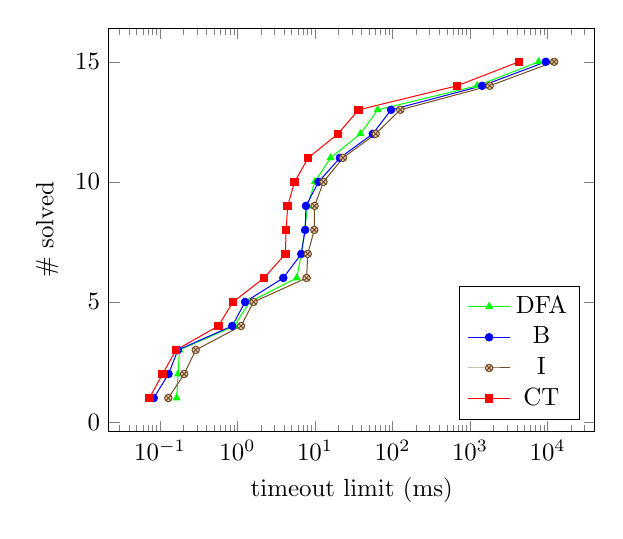
\begin{tikzpicture}[scale=0.9]
      \begin{axis}[
    xmode=log,
    every axis plot/.style={thin},
    xlabel={timeout limit (ms)},
    ylabel={\# solved},
    legend pos=south east
    % table/create on use/cumulative distribution/.style={
    %   create col/expr={\pgfmathaccuma + \thisrow{f(x)}}   
    % }
    ]
    \addplot 
    [mark=triangle*,
    mark size=1.5,
    mark options={solid},
    green] 
    coordinates {
    (0.164, 1)
(0.171, 2)
(0.178, 3)
(0.909, 4)
(1.427, 5)
(5.808, 6)
(6.656, 7)
(7.358, 8)
(8.006, 9)
(9.926, 10)
(15.854, 11)
(38.560, 12)
(64.286, 13)
(1229.552, 14)
(7652.888, 15)
% (1000000.628, 16)
% (1000000.815, 17)
% (1000001.662, 18)
% (1000001.715, 19)
% (1000003.732, 20)
    };

    \addplot 
    [blue,
    mark=*,
    mark size=1.5,
    mark options={solid}]
    coordinates {
    (0.083, 1)
(0.129, 2)
(0.170, 3)
(0.854, 4)
(1.253, 5)
(3.895, 6)
(6.641, 7)
(7.455, 8)
(7.641, 9)
(11.107, 10)
(20.914, 11)
(55.550, 12)
(95.651, 13)
(1430.391, 14)
(9483.710, 15)
% (1000001.612, 16)
% (1000002.108, 17)
% (1000004.667, 18)
% (1000004.816, 19)
% (1000010.248, 20)
    };

    \addplot [brown!60!black,
    mark options={fill=brown!40},
    mark=otimes*,
    mark size=1.5]
    coordinates {
    (0.128, 1)
(0.205, 2)
(0.289, 3)
(1.109, 4)
(1.610, 5)
(7.777, 6)
(8.054, 7)
(9.781, 8)
(9.858, 9)
(12.862, 10)
(22.913, 11)
(60.576, 12)
(125.599, 13)
(1790.063, 14)
(12134.918, 15)
% (1000002.432, 16)
% (1000003.344, 17)
% (1000006.270, 18)
% (1000008.048, 19)
% (1000012.086, 20)
    };

    \addplot 
    [red,
    mark size=1.5,
    mark=square*]
    coordinates {
    (0.073, 1)
(0.108, 2)
(0.161, 3)
(0.565, 4)
(0.875, 5)
(2.203, 6)
(4.143, 7)
(4.237, 8)
(4.437, 9)
(5.452, 10)
(8.171, 11)
(19.749, 12)
(36.412, 13)
(680.323, 14)
(4262.748, 15)
% (1000000.368, 16)
% (1000000.544, 17)
% (1000000.613, 18)
% (1000000.618, 19)
% (1000001.110, 20)
    };
    \legend{DFA,B,I,CT}
  \end{axis}

    \end{tikzpicture}
    \vfill
    \caption{\textbf{Langford 2}.}
    \vspace{\baselineskip}
  \end{minipage}\qquad
\end{figure}

\begin{figure}
  \begin{minipage}[b][10cm][s]{0.45\textwidth}
    \centering
    \vfill
    \begin{tikzpicture}[scale=0.9]
      \begin{axis}[
    xmode=log,
    every axis plot/.style={thin},
    xlabel={timeout limit (ms)},
    ylabel={\% solved},
    legend pos=south east,
    cycle list/Set1-6,
            % define fill color for the marker
            mark list fill={.!75!white},
            mark options={solid},
            cycle multiindex* list={
                Set1-6
                    \nextlist
                [3 of]linestyles
                    \nextlist
                very thick
                \nextlist
                mark=o,
                mark=*,
                mark=square,
                mark=triangle,
                mark=+
            },
    ]

    \addplot
    coordinates {
      (11860, 15)
      (22400, 29)
      (53920, 43)
      (280500, 58)
      
    };
    \addplot
    coordinates {
      (16070, 15)
      (36050, 29)
      (81280, 43)
      (460580, 58)
      
    };
    \addplot
    coordinates {
      (19450, 15)
      (45590, 29)
      (101350, 43)
      (565200, 58)
      
    };
    \addplot
    coordinates {
      (8610, 15)
      (17080, 29)
      (42900, 43)
      (232160, 58)
      
    };
    

    \legend{ DFA, B, I, \textbf{CT} }
  \end{axis}

    \end{tikzpicture}
    \vfill
    \caption{\textbf{Langford 3}.}
    \vspace{\baselineskip}
  \end{minipage}\qquad
  \begin{minipage}[b][10cm][s]{0.45\textwidth}
    \centering
    \vfill
    \begin{tikzpicture}[scale=0.9]
      \begin{axis}[
    xmode=log,
    every axis plot/.style={thin},
    xlabel={timeout limit (ms)},
    ylabel={\% solved},
    legend pos=south east,
    cycle list/Set1-6,
            % define fill color for the marker
            mark list fill={.!75!white},
            mark options={solid},
            cycle multiindex* list={
                Set1-6
                    \nextlist
                [3 of]linestyles
                    \nextlist
                very thick
                \nextlist
                mark=o,
                mark=*,
                mark=square,
                mark=triangle,
                mark=+
            },
    ]

    \addplot
    coordinates {
      (11130, 15)
      (17370, 29)
      (52860, 43)
      (278990, 58)
      
    };
    \addplot
    coordinates {
      (15880, 15)
      (34980, 29)
      (81010, 43)
      (460210, 58)
      
    };
    \addplot
    coordinates {
      (19250, 15)
      (44500, 29)
      (101080, 43)
      (564660, 58)
      
    };
    \addplot
    coordinates {
      (8410, 15)
      (15920, 29)
      (42610, 43)
      (231710, 58)
      
    };
    

    \legend{ DFA, B, I, \textbf{CT} }
  \end{axis}

    \end{tikzpicture}
    \vfill
    \caption{\textbf{Langford 3}.}
    \vspace{\baselineskip}
  \end{minipage}\qquad
\end{figure}

\begin{figure}
  \begin{minipage}[b][10cm][s]{0.45\textwidth}
    \centering
    \vfill
    \begin{tikzpicture}[scale=0.9]
      \begin{axis}[
    xmode=log,
    every axis plot/.style={thin},
    xlabel={timeout limit (ms)},
    ylabel={\% solved},
    legend pos=south east,
    cycle list/Set1-6,
            % define fill color for the marker
            mark list fill={.!75!white},
            mark options={solid},
            cycle multiindex* list={
                Set1-6
                    \nextlist
                [3 of]linestyles
                    \nextlist
                very thick
                \nextlist
                mark=o,
                mark=*,
                mark=square,
                mark=triangle,
                mark=+
            },
    ]

    \addplot
    coordinates {
      (1410, 20)
      (2980, 40)
      (7950, 60)
      (22760, 80)
      (78820, 100)
      
    };
    \addplot
    coordinates {
      (650, 20)
      (1930, 40)
      (7810, 60)
      (29790, 80)
      (124670, 100)
      
    };
    \addplot
    coordinates {
      (740, 20)
      (2300, 40)
      (9460, 60)
      (36010, 80)
      (148310, 100)
      
    };
    \addplot
    coordinates {
      (580, 20)
      (1530, 40)
      (5640, 60)
      (20620, 80)
      (82360, 100)
      
    };
    

    \legend{ DFA, B, I, \textbf{CT} }
  \end{axis}

    \end{tikzpicture}
    \vfill
    \caption{\textbf{Langford 4}.}
    \vspace{\baselineskip}
  \end{minipage}\qquad
  \begin{minipage}[b][10cm][s]{0.45\textwidth}
    \centering
    \vfill
    \begin{tikzpicture}[scale=0.9]
      \begin{axis}[
    xmode=log,
    every axis plot/.style={thin},
    xlabel={timeout limit (ms)},
    ylabel={\% solved},
    legend pos=south east,
    cycle list/Set1-6,
            % define fill color for the marker
            mark list fill={.!75!white},
            mark options={solid},
            cycle multiindex* list={
                Set1-6
                    \nextlist
                [3 of]linestyles
                    \nextlist
                very thick
                \nextlist
                mark=o,
                mark=*,
                mark=square,
                mark=triangle,
                mark=+
            },
    ]

    \addplot
    coordinates {
      (1270, 25)
      (5410, 50)
      (19110, 75)
      (74070, 100)
      
    };
    \addplot
    coordinates {
      (1560, 25)
      (7220, 50)
      (28920, 75)
      (127360, 100)
      
    };
    \addplot
    coordinates {
      (1870, 25)
      (8720, 50)
      (35530, 75)
      (155950, 100)
      
    };
    \addplot
    coordinates {
      (1090, 25)
      (4980, 50)
      (19730, 75)
      (82080, 100)
      
    };
    

    \legend{ DFA, B, I, \textbf{CT} }
  \end{axis}

    \end{tikzpicture}
    \vfill
    \caption{\textbf{Langford 4}.}
    \vspace{\baselineskip}
  \end{minipage}\qquad

\end{figure}

 \begin{figure}

   \begin{minipage}[b][10cm][s]{.45\textwidth}
     \centering
    \vfill
    \begin{tikzpicture}[scale=0.9]
      \begin{axis}[
    xmode=log,
    every axis plot/.style={thin},
    xlabel={timeout limit (ms)},
    ylabel={\% solved},
    legend pos=south east,
    cycle list/Set1-6,
            % define fill color for the marker
            mark list fill={.!75!white},
            mark options={solid},
            cycle multiindex* list={
                Set1-6
                    \nextlist
                [3 of]linestyles
                    \nextlist
                very thick
                \nextlist
                mark=o,
                mark=*,
                mark=square,
                mark=triangle,
                mark=+
            },
    ]

    \addplot
    coordinates {
      (5500, 10)
      (16070, 20)
      (16630, 30)
      (17890, 40)
      (35390, 50)
      (57330, 60)
      (69990, 70)
      (101460, 80)
      (169980, 90)
      (453800, 100)
      
    };
    \addplot
    coordinates {
      (2230, 10)
      (5650, 20)
      (6980, 30)
      (8620, 40)
      (21360, 50)
      (25040, 60)
      (42030, 70)
      (56640, 80)
      (61450, 90)
      (253650, 100)
      
    };
    \addplot
    coordinates {
      (3120, 10)
      (9240, 20)
      (10460, 30)
      (12500, 40)
      (31710, 50)
      (38200, 60)
      (61930, 70)
      (82230, 80)
      (95830, 90)
      (382920, 100)
      
    };
    \addplot
    coordinates {
      (570, 10)
      (1250, 20)
      (1410, 30)
      (1570, 40)
      (3500, 50)
      (3990, 60)
      (6250, 70)
      (8860, 80)
      (10050, 90)
      (42870, 100)
      
    };
    

    \legend{ DFA, B, I, \textbf{CT} }
  \end{axis}

    \end{tikzpicture}    
    \vfill
    \caption{\textbf{Rands JC2500.}}
    \vspace{\baselineskip}
  \end{minipage}\qquad
  \begin{minipage}[b][10cm][s]{.45\textwidth}
    \centering
    \vfill
    \begin{tikzpicture}[scale=0.9]
      \begin{axis}[
    xmode=log,
    every axis plot/.style={thin},
    xlabel={timeout limit (ms)},
    ylabel={\% solved},
    legend pos=south east,
    cycle list/Set1-6,
            % define fill color for the marker
            mark list fill={.!75!white},
            mark options={solid},
            cycle multiindex* list={
                Set1-6
                    \nextlist
                [3 of]linestyles
                    \nextlist
                very thick
                \nextlist
                mark=o,
                mark=*,
                mark=square,
                mark=triangle,
                mark=+
            },
    ]

    \addplot
    coordinates {
      (3940, 10)
      (14500, 20)
      (15100, 30)
      (16350, 40)
      (33840, 50)
      (55800, 60)
      (68450, 70)
      (99900, 80)
      (168430, 90)
      (452240, 100)
      
    };
    \addplot
    coordinates {
      (1990, 10)
      (5420, 20)
      (6750, 30)
      (8390, 40)
      (21120, 50)
      (24800, 60)
      (41790, 70)
      (56410, 80)
      (61210, 90)
      (253400, 100)
      
    };
    \addplot
    coordinates {
      (2890, 10)
      (9000, 20)
      (10220, 30)
      (12270, 40)
      (31480, 50)
      (37970, 60)
      (61700, 70)
      (82000, 80)
      (95600, 90)
      (382660, 100)
      
    };
    \addplot
    coordinates {
      (330, 10)
      (1010, 20)
      (1170, 30)
      (1320, 40)
      (3260, 50)
      (3750, 60)
      (6010, 70)
      (8390, 80)
      (9800, 90)
      (42610, 100)
      
    };
    

    \legend{ DFA, B, I, \textbf{CT} }
  \end{axis}

    \end{tikzpicture}    
    \vfill
    \caption{\textbf{Rands JC2500.}}
    \vspace{\baselineskip}
  \end{minipage}\qquad
\end{figure}

\clearpage

\begin{figure}
  \begin{minipage}[b][10cm][s]{.45\textwidth}
    \centering
    \vfill
    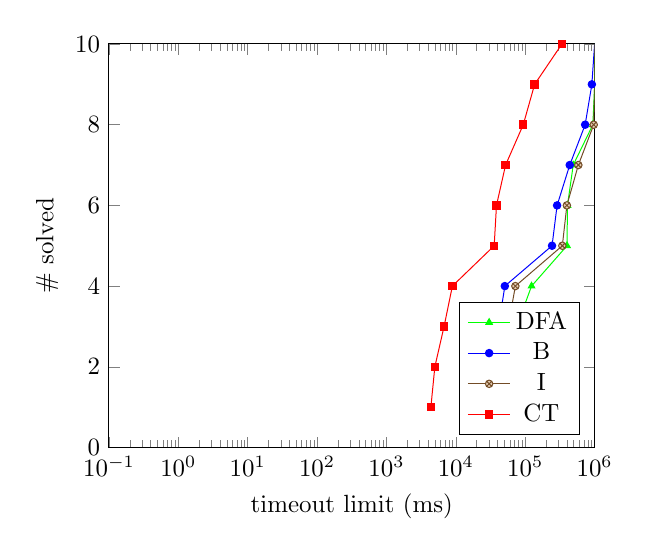
\begin{tikzpicture}[scale=0.9]
      \begin{axis}[
    xmode=log,
    ymin=0,ymax=10,
    xmin=0.1, xmax=1000000,
    every axis plot/.style={thin},
    xlabel={timeout limit (ms)},
    ylabel={\# solved},
    legend pos=south east
    % table/create on use/cumulative distribution/.style={
    %   create col/expr={\pgfmathaccuma + \thisrow{f(x)}}   
    % }
    ]
    \addplot 
    [mark=triangle*,
    mark size=1.5,
    mark options={solid},
    green] 
    coordinates {
    (37271.407, 1)
(63329.760, 2)
(75340.967, 3)
(123361.614, 4)
(400331.140, 5)
(406374.082, 6)
(491965.258, 7)
(943701.318, 8)
(1003127.715, 9)
(1003191.173, 10)
    };

    \addplot 
    [blue,
    mark=*,
    mark size=1.5,
    mark options={solid}]
    coordinates {
    (23487.263, 1)
(31493.067, 2)
(41324.456, 3)
(50843.172, 4)
(243499.863, 5)
(288078.384, 6)
(438078.025, 7)
(731291.713, 8)
(912991.209, 9)
(1000435.280, 10)
    };

    \addplot [brown!60!black,
    mark options={fill=brown!40},
    mark=otimes*,
    mark size=1.5]
    coordinates {
    (31721.470, 1)
(45760.945, 2)
(56699.417, 3)
(72142.510, 4)
(342690.713, 5)
(398501.909, 6)
(583027.925, 7)
(971126.357, 8)
(1000434.235, 9)
(1000435.846, 10)
    };

    \addplot 
    [red,
    mark size=1.5,
    mark=square*]
    coordinates {
    (4367.654, 1)
(4983.151, 2)
(6770.036, 3)
(8914.062, 4)
(35712.233, 5)
(38524.930, 6)
(52111.274, 7)
(93677.132, 8)
(136706.431, 9)
(338099.921, 10)
    };
    \legend{DFA,B,I,CT}
  \end{axis}

    \end{tikzpicture}
    \vfill
    \caption{\textbf{Rands JC5000.}}
    \vspace{\baselineskip}
  \end{minipage}\qquad
  \begin{minipage}[b][10cm][s]{.45\textwidth}
    \centering
    \vfill
    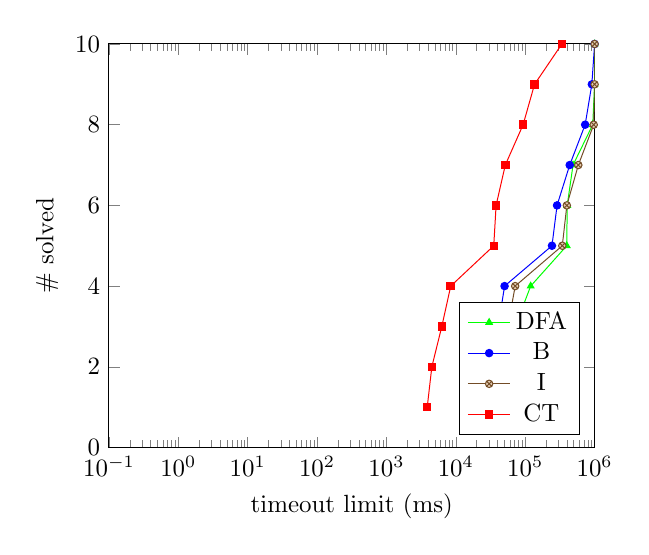
\begin{tikzpicture}[scale=0.9]
      \begin{axis}[
    xmode=log,
    ymin=0,ymax=10,
    xmin=0.1, xmax=1000000,
    every axis plot/.style={thin},
    xlabel={timeout limit (ms)},
    ylabel={\# solved},
    legend pos=south east
    % table/create on use/cumulative distribution/.style={
    %   create col/expr={\pgfmathaccuma + \thisrow{f(x)}}   
    % }
    ]
    \addplot 
    [mark=triangle*,
    mark size=1.5,
    mark options={solid},
    green] 
    coordinates {
    (33755.099, 1)
(59802.836, 2)
(71937.877, 3)
(119806.483, 4)
(396881.609, 5)
(402866.818, 6)
(488432.740, 7)
(940241.994, 8)
(1000000.748, 9)
(1000002.972, 10)
    };

    \addplot 
    [blue,
    mark=*,
    mark size=1.5,
    mark options={solid}]
    coordinates {
    (23034.750, 1)
(31048.019, 2)
(40866.833, 3)
(50387.285, 4)
(243052.362, 5)
(287588.066, 6)
(437627.533, 7)
(730831.980, 8)
(912534.058, 9)
(1000002.047, 10)
    };

    \addplot [brown!60!black,
    mark options={fill=brown!40},
    mark=otimes*,
    mark size=1.5]
    coordinates {
    (31269.341, 1)
(45316.136, 2)
(56241.728, 3)
(71678.111, 4)
(342240.509, 5)
(398047.029, 6)
(582574.149, 7)
(970690.640, 8)
(1000000.563, 9)
(1000001.419, 10)
    };

    \addplot 
    [red,
    mark size=1.5,
    mark=square*]
    coordinates {
    (3869.207, 1)
(4510.441, 2)
(6278.130, 3)
(8440.271, 4)
(35190.733, 5)
(38053.208, 6)
(51613.207, 7)
(93224.815, 8)
(136257.056, 9)
(337657.155, 10)
    };
    \legend{DFA,B,I,CT}
  \end{axis}

    \end{tikzpicture}
    \vfill
    \caption{\textbf{Rands JC5000.}}
    \vspace{\baselineskip}
  \end{minipage}\qquad
\end{figure}

\begin{figure}
    \begin{minipage}[b][10cm][s]{.45\textwidth}
    \centering
    \vfill
    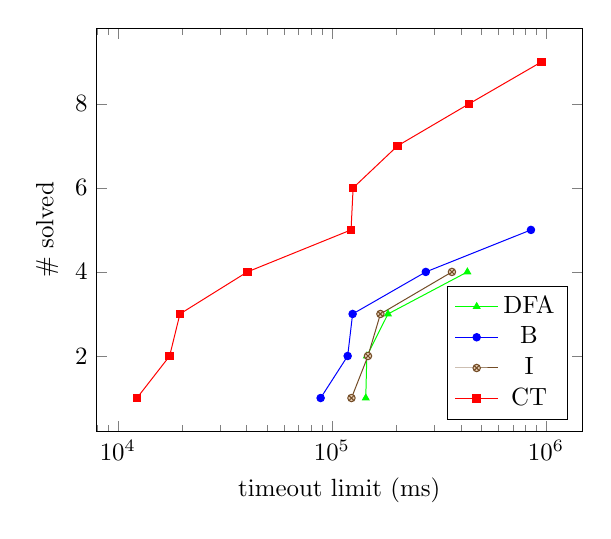
\begin{tikzpicture}[scale=0.9]
      \begin{axis}[
    xmode=log,
    every axis plot/.style={thin},
    xlabel={timeout limit (ms)},
    ylabel={\# solved},
    legend pos=south east
    % table/create on use/cumulative distribution/.style={
    %   create col/expr={\pgfmathaccuma + \thisrow{f(x)}}   
    % }
    ]
    \addplot 
    [mark=triangle*,
    mark size=1.5,
    mark options={solid},
    green] 
    coordinates {
    (143986.214, 1)
(145624.128, 2)
(182844.931, 3)
(429527.079, 4)
% (1004920.333, 5)
% (1005091.406, 6)
% (1005121.020, 7)
% (1005141.458, 8)
% (1005180.694, 9)
% (1005181.896, 10)
    };

    \addplot 
    [blue,
    mark=*,
    mark size=1.5,
    mark options={solid}]
    coordinates {
    (88610.730, 1)
(118513.380, 2)
(124991.902, 3)
(274645.919, 4)
(851285.302, 5)
% (1000662.235, 6)
% (1000665.157, 7)
% (1000667.124, 8)
% (1000679.084, 9)
% (1000680.879, 10)
    };

    \addplot [brown!60!black,
    mark options={fill=brown!40},
    mark=otimes*,
    mark size=1.5]
    coordinates {
    (123456.088, 1)
(147458.027, 2)
(168559.303, 3)
(363926.326, 4)
% (1000644.518, 5)
% (1000648.628, 6)
% (1000660.653, 7)
% (1000663.644, 8)
% (1000669.943, 9)
% (1000672.172, 10)
    };

    \addplot 
    [red,
    mark size=1.5,
    mark=square*]
    coordinates {
    (12283.482, 1)
(17462.103, 2)
(19503.895, 3)
(40266.047, 4)
(122893.209, 5)
(125673.584, 6)
(202682.066, 7)
(437565.193, 8)
(955387.007, 9)
%(1000911.643, 10)
    };
    \legend{DFA,B,I,CT}
  \end{axis}

    \end{tikzpicture}
    \vfill
    \caption{\textbf{Rands JC7500}.}
    \vspace{\baselineskip}
  \end{minipage}\qquad
  \begin{minipage}[b][10cm][s]{.45\textwidth}
    \centering
    \vfill
    \begin{tikzpicture}[scale=0.9]
      \begin{axis}[
    xmode=log,
    every axis plot/.style={thin},
    xlabel={timeout limit (ms)},
    ylabel={\% solved},
    legend pos=south east,
    cycle list/Set1-6,
            % define fill color for the marker
            mark list fill={.!75!white},
            mark options={solid},
            cycle multiindex* list={
                Set1-6
                    \nextlist
                [3 of]linestyles
                    \nextlist
                very thick
                \nextlist
                mark=o,
                mark=*,
                mark=square,
                mark=triangle,
                mark=+
            },
    ]

    \addplot
    coordinates {
      (136770, 10)
      (142590, 20)
      (184110, 30)
      (435120, 40)
      
    };
    \addplot
    coordinates {
      (81100, 10)
      (105010, 20)
      (117160, 30)
      (259290, 40)
      (777090, 50)
      (900680, 60)
      
    };
    \addplot
    coordinates {
      (112900, 10)
      (136490, 20)
      (156280, 30)
      (341990, 40)
      
    };
    \addplot
    coordinates {
      (7060, 10)
      (10860, 20)
      (11760, 30)
      (25300, 40)
      (71730, 50)
      (80130, 60)
      (132930, 70)
      (275110, 80)
      (622520, 90)
      
    };
    

    \legend{ DFA, B, I, \textbf{CT} }
  \end{axis}

    \end{tikzpicture}
    \vfill
    \caption{\textbf{Rands JC7500}.}
    \vspace{\baselineskip}
  \end{minipage}\qquad
\end{figure}

\begin{figure}
  \begin{minipage}[b][10cm][s]{.45\textwidth}
    \centering
    \vfill
    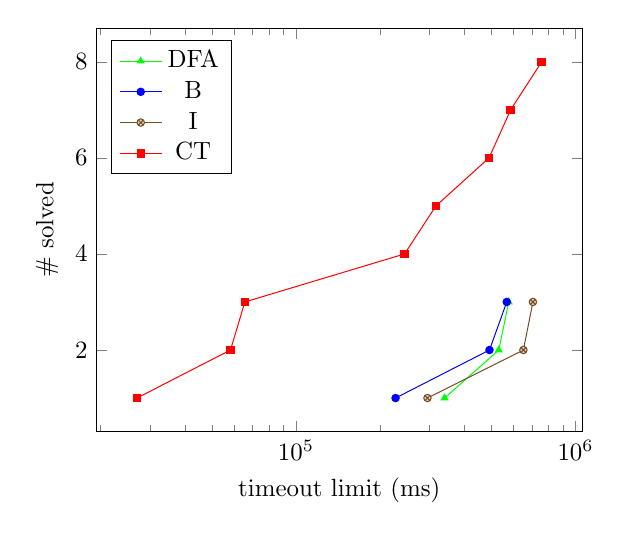
\begin{tikzpicture}[scale=0.9]
      \begin{axis}[
    xmode=log,
    every axis plot/.style={thin},
    xlabel={timeout limit (ms)},
    ylabel={\# solved},
    legend pos=north west
    % table/create on use/cumulative distribution/.style={
    %   create col/expr={\pgfmathaccuma + \thisrow{f(x)}}   
    % }
    ]
    \addplot 
    [mark=triangle*,
    mark size=1.5,
    mark options={solid},
    green] 
    coordinates {
    (339960.449, 1)
(531357.500, 2)
(576758.002, 3)
% (1006830.253, 4)
% (1006953.686, 5)
% (1006987.278, 6)
% (1007012.182, 7)
% (1007040.479, 8)
% (1007166.422, 9)
% (1007385.382, 10)
    };

    \addplot 
    [blue,
    mark=*,
    mark size=1.5,
    mark options={solid}]
    coordinates {
    (227052.199, 1)
(492242.811, 2)
(567372.313, 3)
% (1000877.234, 4)
% (1000889.042, 5)
% (1000892.874, 6)
% (1000895.207, 7)
% (1000911.856, 8)
% (1000913.878, 9)
% (1000928.789, 10)
    };

    \addplot [brown!60!black,
    mark options={fill=brown!40},
    mark=otimes*,
    mark size=1.5]
    coordinates {
    (295287.152, 1)
(650810.991, 2)
(703794.608, 3)
% (1000887.426, 4)
% (1000895.815, 5)
% (1000897.600, 6)
% (1000901.551, 7)
% (1000905.923, 8)
% (1000907.888, 9)
% (1000913.436, 10)
    };

    \addplot 
    [red,
    mark size=1.5,
    mark=square*]
    coordinates {
    (26984.703, 1)
(58304.179, 2)
(65624.179, 3)
(244616.117, 4)
(316746.918, 5)
(490346.243, 6)
(586068.768, 7)
(756641.057, 8)
%(1001171.576, 9)
%(1001192.839, 10)
    };
    \legend{DFA,B,I,CT}
  \end{axis}

    \end{tikzpicture}
    \vfill
    \caption{\textbf{Rands JC10000}.}
    \vspace{\baselineskip}
  \end{minipage}\qquad
  \begin{minipage}[b][10cm][s]{.45\textwidth}
    \centering
    \vfill
    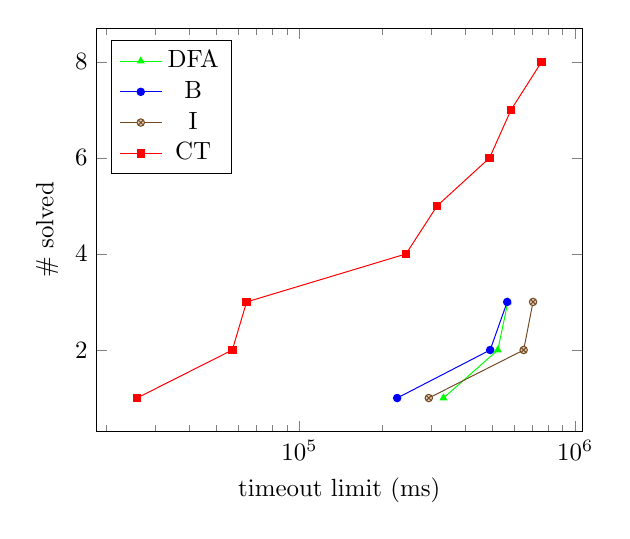
\begin{tikzpicture}[scale=0.9]
      \begin{axis}[
    xmode=log,
    every axis plot/.style={thin},
    xlabel={timeout limit (ms)},
    ylabel={\# solved},
    legend pos=north west
    % table/create on use/cumulative distribution/.style={
    %   create col/expr={\pgfmathaccuma + \thisrow{f(x)}}   
    % }
    ]
    \addplot 
    [mark=triangle*,
    mark size=1.5,
    mark options={solid},
    green] 
    coordinates {
    (332745.543, 1)
(523863.709, 2)
(569686.426, 3)
% (1000000.172, 4)
% (1000000.554, 5)
% (1000000.920, 6)
% (1000001.037, 7)
% (1000001.490, 8)
% (1000002.276, 9)
% (1000003.312, 10)
    };

    \addplot 
    [blue,
    mark=*,
    mark size=1.5,
    mark options={solid}]
    coordinates {
    (226152.398, 1)
(491387.804, 2)
(566477.841, 3)
% (1000000.822, 4)
% (1000001.468, 5)
% (1000001.597, 6)
% (1000001.921, 7)
% (1000002.047, 8)
% (1000002.465, 9)
% (1000003.238, 10)
    };

    \addplot [brown!60!black,
    mark options={fill=brown!40},
    mark=otimes*,
    mark size=1.5]
    coordinates {
    (294414.233, 1)
(649951.472, 2)
(702865.808, 3)
% (1000000.517, 4)
% (1000000.699, 5)
% (1000000.802, 6)
% (1000001.295, 7)
% (1000001.350, 8)
% (1000001.480, 9)
% (1000001.637, 10)
    };

    \addplot 
    [red,
    mark size=1.5,
    mark=square*]
    coordinates {
    (25774.100, 1)
(57124.920, 2)
(64359.631, 3)
(243389.037, 4)
(315549.601, 5)
(489096.976, 6)
(584890.320, 7)
(755476.499, 8)
%(1000000.186, 9)
%(1000000.225, 10)
    };
    \legend{DFA,B,I,CT}
  \end{axis}

    \end{tikzpicture}
    \vfill
    \caption{\textbf{Rands JC10000}.}
    \vspace{\baselineskip}
  \end{minipage}\qquad

\end{figure}

\clearpage

\begin{figure}
  
  \begin{minipage}[b][10cm][s]{0.45\textwidth}
    \centering
    \vfill
    \begin{tikzpicture}[scale=0.9]
      \begin{axis}[
    xmode=log,
    every axis plot/.style={thin},
    xlabel={timeout limit (ms)},
    ylabel={\% solved},
    legend pos=south east,
    cycle list/Set1-6,
            % define fill color for the marker
            mark list fill={.!75!white},
            mark options={solid},
            cycle multiindex* list={
                Set1-6
                    \nextlist
                [3 of]linestyles
                    \nextlist
                very thick
                \nextlist
                mark=o,
                mark=*,
                mark=square,
                mark=triangle,
                mark=+
            },
    ]

    \addplot
    coordinates {
      (2550, 34)
      (4320, 67)
      (7020, 100)
      
    };
    \addplot
    coordinates {
      (2410, 34)
      (4300, 67)
      (7300, 100)
      
    };
    \addplot
    coordinates {
      (3770, 34)
      (6470, 67)
      (11240, 100)
      
    };
    \addplot
    coordinates {
      (1950, 34)
      (2830, 67)
      (4690, 100)
      
    };
    

    \legend{ DFA, B, I, \textbf{CT} }
  \end{axis}

    \end{tikzpicture}
    \vfill
    \caption{\textbf{AIM-50}.}
    \vspace{\baselineskip}
  \end{minipage}\qquad

  \begin{minipage}[b][10cm][s]{0.45\textwidth}
    \centering
    \vfill
    \begin{tikzpicture}[scale=0.9]
      \begin{axis}[
    xmode=log,
    every axis plot/.style={thin},
    xlabel={timeout limit (ms)},
    ylabel={\% solved},
    legend pos=south east,
    cycle list/Set1-6,
            % define fill color for the marker
            mark list fill={.!75!white},
            mark options={solid},
            cycle multiindex* list={
                Set1-6
                    \nextlist
                [3 of]linestyles
                    \nextlist
                very thick
                \nextlist
                mark=o,
                mark=*,
                mark=square,
                mark=triangle,
                mark=+
            },
    ]

    \addplot
    coordinates {
      (10, 100)
      
    };
    \addplot
    coordinates {
      (2400, 34)
      (4310, 67)
      (7210, 100)
      
    };
    \addplot
    coordinates {
      (3720, 34)
      (6470, 67)
      (11170, 100)
      
    };
    \addplot
    coordinates {
      (1780, 34)
      (2680, 67)
      (4360, 100)
      
    };
    

    \legend{ DFA, B, I, \textbf{CT} }
  \end{axis}

    \end{tikzpicture}
    \vfill
    \caption{\textbf{AIM-50}.}
    \vspace{\baselineskip}
  \end{minipage}\qquad
\end{figure}

\begin{figure}
  \begin{minipage}[b][10cm][s]{0.45\textwidth}
    \centering
    \vfill
    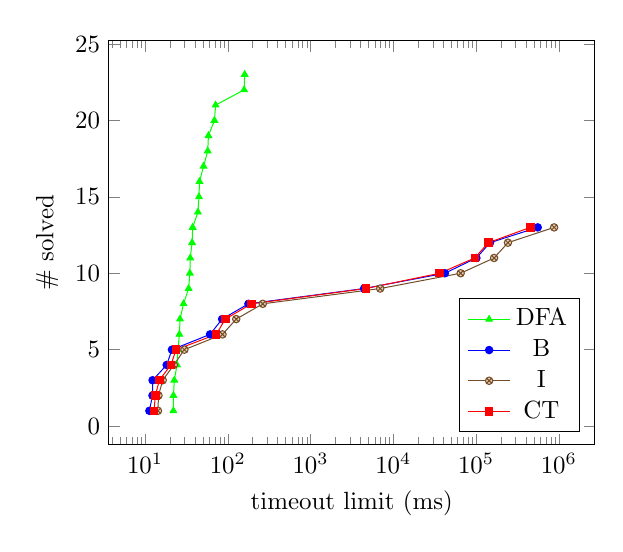
\begin{tikzpicture}[scale=0.9]
      \begin{axis}[
    xmode=log,
    every axis plot/.style={thin},
    xlabel={timeout limit (ms)},
    ylabel={\# solved},
    legend pos=south east
    % table/create on use/cumulative distribution/.style={
    %   create col/expr={\pgfmathaccuma + \thisrow{f(x)}}   
    % }
    ]
    \addplot 
    [mark=triangle*,
    mark size=1.5,
    mark options={solid},
    green] 
    coordinates {
    (21.989, 1)
(22.041, 2)
(22.559, 3)
(24.331, 4)
(24.974, 5)
(26.007, 6)
(26.462, 7)
(29.157, 8)
(33.602, 9)
(34.800, 10)
(35.158, 11)
(37.017, 12)
(37.604, 13)
(43.531, 14)
(44.847, 15)
(45.476, 16)
(50.917, 17)
(57.169, 18)
(58.349, 19)
(68.896, 20)
(71.202, 21)
(157.413, 22)
(159.802, 23)
    };

    \addplot 
    [blue,
    mark=*,
    mark size=1.5,
    mark options={solid}]
    coordinates {
    (11.281, 1)
(12.293, 2)
(12.323, 3)
(18.245, 4)
(21.125, 5)
(61.006, 6)
(85.311, 7)
(177.463, 8)
(4439.520, 9)
(41952.782, 10)
(100937.940, 11)
(147496.534, 12)
(556008.284, 13)
% (1000003.406, 14)
% (1000003.522, 15)
% (1000003.551, 16)
% (1000003.690, 17)
% (1000003.713, 18)
% (1000003.866, 19)
% (1000003.877, 20)
% (1000004.136, 21)
% (1000004.172, 22)
% (1000004.261, 23)
    };

    \addplot [brown!60!black,
    mark options={fill=brown!40},
    mark=otimes*,
    mark size=1.5]
    coordinates {
    (14.319, 1)
(14.525, 2)
(16.358, 3)
(22.251, 4)
(29.907, 5)
(86.300, 6)
(126.361, 7)
(264.396, 8)
(6937.110, 9)
(65105.320, 10)
(165084.246, 11)
(242777.983, 12)
(877449.095, 13)
% (1000004.285, 14)
% (1000004.482, 15)
% (1000004.500, 16)
% (1000004.632, 17)
% (1000004.858, 18)
% (1000004.869, 19)
% (1000004.994, 20)
% (1000015.307, 21)
% (1000021.218, 22)
% (1000094.474, 23)
    };

    \addplot 
    [red,
    mark size=1.5,
    mark=square*]
    coordinates {
    (12.839, 1)
(13.309, 2)
(14.887, 3)
(20.483, 4)
(23.742, 5)
(72.390, 6)
(93.185, 7)
(193.329, 8)
(4643.160, 9)
(36315.326, 10)
(96472.476, 11)
(140766.972, 12)
(452413.350, 13)
% (1000004.885, 14)
% (1000005.183, 15)
% (1000005.227, 16)
% (1000005.436, 17)
% (1000005.455, 18)
% (1000005.543, 19)
% (1000009.510, 20)
% (1000018.333, 21)
% (1000020.654, 22)
% (1000126.631, 23)
    };
    \legend{DFA,B,I,CT}
  \end{axis}

    \end{tikzpicture}
    \vfill
    \caption{\textbf{AIM-100}.}
    \vspace{\baselineskip}
  \end{minipage}\qquad
  \begin{minipage}[b][10cm][s]{0.45\textwidth}
    \centering
    \vfill
    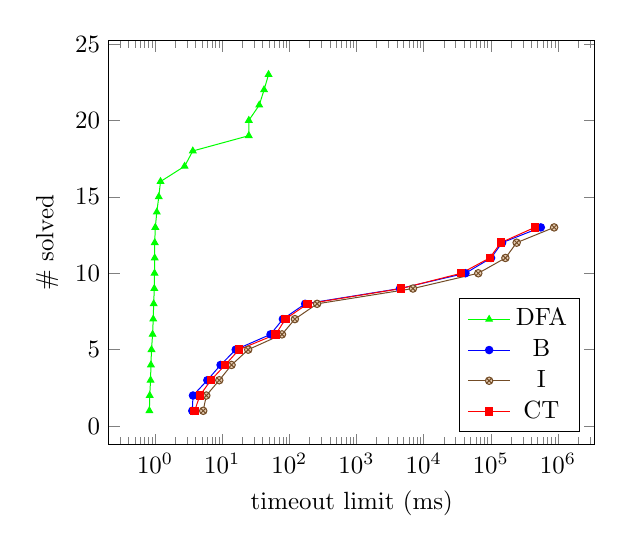
\begin{tikzpicture}[scale=0.9]
      \begin{axis}[
    xmode=log,
    every axis plot/.style={thin},
    xlabel={timeout limit (ms)},
    ylabel={\# solved},
    legend pos=south east
    % table/create on use/cumulative distribution/.style={
    %   create col/expr={\pgfmathaccuma + \thisrow{f(x)}}   
    % }
    ]
    \addplot 
    [mark=triangle*,
    mark size=1.5,
    mark options={solid},
    green] 
    coordinates {
    (0.823, 1)
(0.832, 2)
(0.857, 3)
(0.867, 4)
(0.885, 5)
(0.918, 6)
(0.939, 7)
(0.953, 8)
(0.974, 9)
(0.981, 10)
(0.987, 11)
(0.988, 12)
(1.008, 13)
(1.061, 14)
(1.135, 15)
(1.205, 16)
(2.753, 17)
(3.647, 18)
(24.877, 19)
(24.886, 20)
(35.599, 21)
(42.011, 22)
(48.965, 23)
    };

    \addplot 
    [blue,
    mark=*,
    mark size=1.5,
    mark options={solid}]
    coordinates {
    (3.586, 1)
(3.671, 2)
(6.004, 3)
(9.450, 4)
(15.887, 5)
(52.426, 6)
(80.095, 7)
(171.902, 8)
(4436.194, 9)
(41949.006, 10)
(100934.221, 11)
(147492.566, 12)
(556004.535, 13)
% (1000000.165, 14)
% (1000000.167, 15)
% (1000000.174, 16)
% (1000000.174, 17)
% (1000000.176, 18)
% (1000000.179, 19)
% (1000000.202, 20)
% (1000000.260, 21)
% (1000000.266, 22)
% (1000000.286, 23)
    };

    \addplot [brown!60!black,
    mark options={fill=brown!40},
    mark=otimes*,
    mark size=1.5]
    coordinates {
    (5.211, 1)
(5.793, 2)
(9.033, 3)
(13.782, 4)
(24.369, 5)
(77.669, 6)
(120.860, 7)
(258.984, 8)
(6933.488, 9)
(65101.206, 10)
(165079.465, 11)
(242773.103, 12)
(877436.255, 13)
% (1000000.113, 14)
% (1000000.118, 15)
% (1000000.123, 16)
% (1000000.132, 17)
% (1000000.154, 18)
% (1000000.165, 19)
% (1000000.189, 20)
% (1000000.191, 21)
% (1000000.196, 22)
% (1000000.259, 23)
    };

    \addplot 
    [red,
    mark size=1.5,
    mark=square*]
    coordinates {
    (3.886, 1)
(4.643, 2)
(6.772, 3)
(11.080, 4)
(17.750, 5)
(62.656, 6)
(87.179, 7)
(187.117, 8)
(4632.128, 9)
(36310.893, 10)
(96431.551, 11)
(140762.037, 12)
(452408.039, 13)
% (1000000.102, 14)
% (1000000.115, 15)
% (1000000.118, 16)
% (1000000.134, 17)
% (1000000.137, 18)
% (1000000.157, 19)
% (1000000.200, 20)
% (1000000.202, 21)
% (1000000.221, 22)
% (1000000.239, 23)
    };
    \legend{DFA,B,I,CT}
  \end{axis}

    \end{tikzpicture}
    \vfill
    \caption{\textbf{AIM-100}.}
    \vspace{\baselineskip}
  \end{minipage}\qquad
\end{figure}

\begin{figure}
  \begin{minipage}[b][10cm][s]{0.45\textwidth}
    \centering
    \vfill
    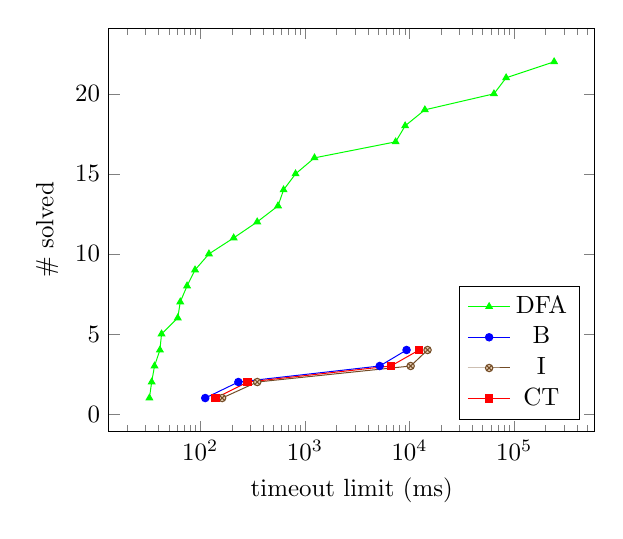
\begin{tikzpicture}[scale=0.9]
      \begin{axis}[
    xmode=log,
    every axis plot/.style={thin},
    xlabel={timeout limit (ms)},
    ylabel={\# solved},
    legend pos=south east
    % table/create on use/cumulative distribution/.style={
    %   create col/expr={\pgfmathaccuma + \thisrow{f(x)}}   
    % }
    ]
    \addplot 
    [mark=triangle*,
    mark size=1.5,
    mark options={solid},
    green] 
    coordinates {
    (32.646, 1)
(34.322, 2)
(36.539, 3)
(41.139, 4)
(42.637, 5)
(60.923, 6)
(64.362, 7)
(74.768, 8)
(89.108, 9)
(121.012, 10)
(208.525, 11)
(350.032, 12)
(553.291, 13)
(625.153, 14)
(813.725, 15)
(1234.205, 16)
(7361.018, 17)
(9076.992, 18)
(14005.709, 19)
(64038.325, 20)
(83738.459, 21)
(240798.763, 22)
    };

    \addplot 
    [blue,
    mark=*,
    mark size=1.5,
    mark options={solid}]
    coordinates {
    (111.532, 1)
(231.223, 2)
(5185.609, 3)
(9363.587, 4)
% (1000006.135, 5)
% (1000006.157, 6)
% (1000006.188, 7)
% (1000006.300, 8)
% (1000006.306, 9)
% (1000007.024, 10)
% (1000007.087, 11)
% (1000007.302, 12)
% (1000007.563, 13)
% (1000010.560, 14)
% (1000010.850, 15)
% (1000046.435, 16)
% (1000167.771, 17)
% (1001173.564, 18)
% (1006453.700, 19)
% (1008543.597, 20)
% (1010562.071, 21)
% (1019241.202, 22)
    };

    \addplot [brown!60!black,
    mark options={fill=brown!40},
    mark=otimes*,
    mark size=1.5]
    coordinates {
    (161.801, 1)
(350.376, 2)
(10244.105, 3)
(14856.666, 4)
% (1000007.483, 5)
% (1000007.625, 6)
% (1000007.695, 7)
% (1000008.729, 8)
% (1000009.950, 9)
% (1000011.262, 10)
% (1000019.536, 11)
% (1000023.192, 12)
% (1000025.767, 13)
% (1000040.365, 14)
% (1000041.636, 15)
% (1000051.012, 16)
% (1000053.849, 17)
% (1000118.768, 18)
% (1000166.508, 19)
% (1000467.387, 20)
% (1001776.595, 21)
% (1015356.678, 22)
    };

    \addplot 
    [red,
    mark size=1.5,
    mark=square*]
    coordinates {
    (140.045, 1)
(284.098, 2)
(6638.875, 3)
(12352.151, 4)
% (1000007.437, 5)
% (1000007.976, 6)
% (1000009.059, 7)
% (1000009.398, 8)
% (1000009.787, 9)
% (1000013.785, 10)
% (1000024.236, 11)
% (1000038.306, 12)
% (1000061.649, 13)
% (1000067.115, 14)
% (1000073.775, 15)
% (1000110.045, 16)
% (1000202.940, 17)
% (1000283.824, 18)
% (1001241.998, 19)
% (1012931.719, 20)
% (1016410.000, 21)
% (1021392.559, 22)
    };
    \legend{DFA,B,I,CT}
  \end{axis}

    \end{tikzpicture}
    \vfill
    \caption{\textbf{AIM-200}.}
    \vspace{\baselineskip}
  \end{minipage}\qquad
  \begin{minipage}[b][10cm][s]{0.45\textwidth}
    \centering
    \vfill
    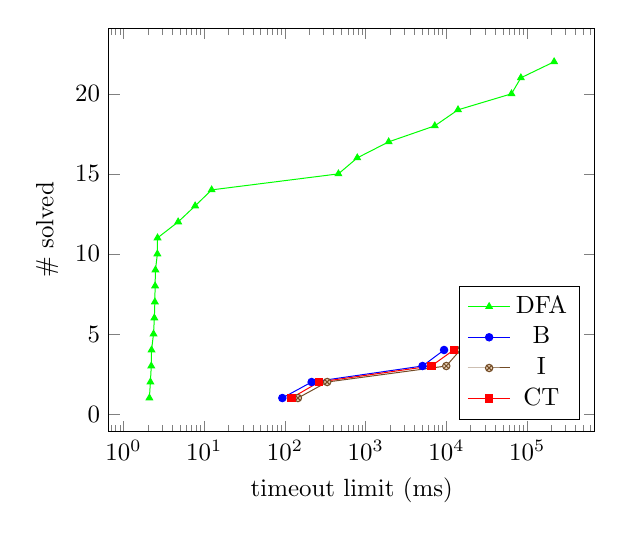
\begin{tikzpicture}[scale=0.9]
      \begin{axis}[
    xmode=log,
    every axis plot/.style={thin},
    xlabel={timeout limit (ms)},
    ylabel={\# solved},
    legend pos=south east
    % table/create on use/cumulative distribution/.style={
    %   create col/expr={\pgfmathaccuma + \thisrow{f(x)}}   
    % }
    ]
    \addplot 
    [mark=triangle*,
    mark size=1.5,
    mark options={solid},
    green] 
    coordinates {
    (2.092, 1)
(2.153, 2)
(2.207, 3)
(2.224, 4)
(2.353, 5)
(2.410, 6)
(2.444, 7)
(2.462, 8)
(2.486, 9)
(2.626, 10)
(2.638, 11)
(4.751, 12)
(7.714, 13)
(12.349, 14)
(459.348, 15)
(786.654, 16)
(1926.845, 17)
(7178.726, 18)
(13920.549, 19)
(63961.995, 20)
(83629.587, 21)
(215920.851, 22)
    };

    \addplot 
    [blue,
    mark=*,
    mark size=1.5,
    mark options={solid}]
    coordinates {
    (92.762, 1)
(214.140, 2)
(5059.466, 3)
(9347.039, 4)
% (1000000.212, 5)
% (1000000.214, 6)
% (1000000.230, 7)
% (1000000.234, 8)
% (1000000.236, 9)
% (1000000.243, 10)
% (1000000.247, 11)
% (1000000.332, 12)
% (1000000.348, 13)
% (1000000.356, 14)
% (1000000.384, 15)
% (1000000.413, 16)
% (1000000.580, 17)
% (1001526.960, 18)
% (1013587.491, 19)
% (1015726.858, 20)
% (1021700.000, 21)
% (1026780.972, 22)
    };

    \addplot [brown!60!black,
    mark options={fill=brown!40},
    mark=otimes*,
    mark size=1.5]
    coordinates {
    (144.623, 1)
(333.321, 2)
(9960.406, 3)
(14839.411, 4)
%(1000000.132, 5)
% (1000000.132, 6)
% (1000000.138, 7)
% (1000000.154, 8)
% (1000000.156, 9)
% (1000000.161, 10)
% (1000000.176, 11)
% (1000000.201, 12)
% (1000000.233, 13)
% (1000000.233, 14)
% (1000000.264, 15)
% (1000000.302, 16)
% (1000000.338, 17)
% (1000000.401, 18)
% (1000000.462, 19)
% (1000000.559, 20)
% (1000201.313, 21)
% (1030367.681, 22)
    };

    \addplot 
    [red,
    mark size=1.5,
    mark=square*]
    coordinates {
    (120.173, 1)
(264.364, 2)
(6492.284, 3)
(12332.389, 4)
% (1000000.117, 5)
% (1000000.130, 6)
% (1000000.138, 7)
% (1000000.141, 8)
% (1000000.144, 9)
% (1000000.148, 10)
% (1000000.157, 11)
% (1000000.179, 12)
% (1000000.199, 13)
% (1000000.223, 14)
% (1000000.258, 15)
% (1000000.312, 16)
% (1000000.349, 17)
% (1000000.387, 18)
% (1000000.408, 19)
% (1019145.714, 20)
% (1021004.571, 21)
% (1051023.598, 22)
    };
    \legend{DFA,B,I,CT}
  \end{axis}

    \end{tikzpicture}
    \vfill
    \caption{\textbf{AIM-200}.}
    \vspace{\baselineskip}
  \end{minipage}\qquad
\end{figure}

\clearpage

\begin{figure}
  \begin{minipage}[b][10cm][s]{0.45\textwidth}
    \centering
    \vfill
    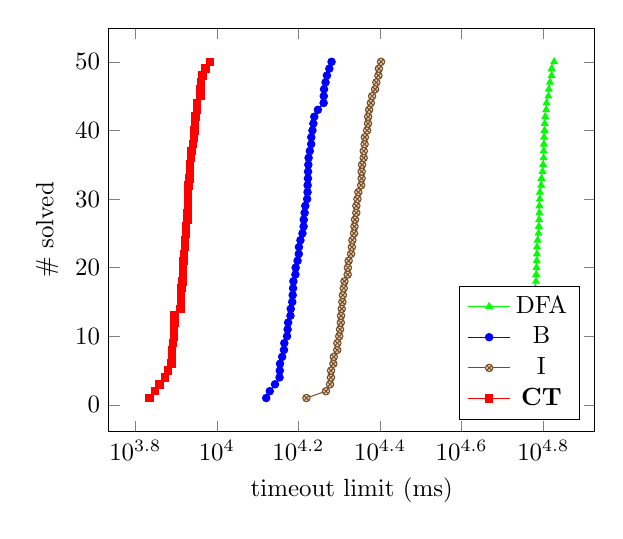
\begin{tikzpicture}[scale=0.9]
      \begin{axis}[
    xmode=log,
    every axis plot/.style={thin},
    xlabel={timeout limit (ms)},
    ylabel={\# solved},
    legend pos=south east
    % table/create on use/cumulative distribution/.style={
    %   create col/expr={\pgfmathaccuma + \thisrow{f(x)}}   
    % }
    ]
    \addplot 
    [mark=triangle*,
    mark size=1.5,
    mark options={solid},
    green] 
    coordinates {
    (51125.785, 1)
(54263.257, 2)
(56487.527, 3)
(56702.786, 4)
(56985.792, 5)
(57276.885, 6)
(57622.584, 7)
(58132.270, 8)
(58140.300, 9)
(58355.175, 10)
(58676.203, 11)
(59158.883, 12)
(59632.816, 13)
(59713.900, 14)
(59728.215, 15)
(60269.934, 16)
(60313.648, 17)
(60549.505, 18)
(60622.637, 19)
(60711.449, 20)
(60810.980, 21)
(60862.784, 22)
(60914.293, 23)
(61100.454, 24)
(61428.994, 25)
(61523.477, 26)
(61625.366, 27)
(61712.915, 28)
(61729.236, 29)
(61886.596, 30)
(61900.845, 31)
(62341.893, 32)
(62455.546, 33)
(62817.572, 34)
(63010.646, 35)
(63184.232, 36)
(63221.376, 37)
(63304.994, 38)
(63379.424, 39)
(63540.272, 40)
(63613.419, 41)
(63781.589, 42)
(64128.455, 43)
(64263.902, 44)
(64924.220, 45)
(65113.900, 46)
(65508.695, 47)
(66133.866, 48)
(66157.482, 49)
(67076.860, 50)
    };

    \addplot 
    [blue,
    mark=*,
    mark size=1.5,
    mark options={solid}]
    coordinates {
    (13210.645, 1)
(13478.699, 2)
(13880.904, 3)
(14240.906, 4)
(14262.586, 5)
(14281.012, 6)
(14453.879, 7)
(14601.257, 8)
(14630.915, 9)
(14856.229, 10)
(14906.587, 11)
(14947.426, 12)
(15147.432, 13)
(15173.599, 14)
(15300.351, 15)
(15338.350, 16)
(15370.471, 17)
(15400.162, 18)
(15575.398, 19)
(15599.555, 20)
(15767.367, 21)
(15876.487, 22)
(15890.540, 23)
(16026.936, 24)
(16207.081, 25)
(16313.213, 26)
(16328.178, 27)
(16410.911, 28)
(16468.425, 29)
(16641.910, 30)
(16678.794, 31)
(16689.212, 32)
(16716.749, 33)
(16728.322, 34)
(16755.929, 35)
(16780.814, 36)
(16896.779, 37)
(17026.619, 38)
(17037.921, 39)
(17147.387, 40)
(17237.324, 41)
(17326.549, 42)
(17685.575, 43)
(18266.956, 44)
(18281.157, 45)
(18310.293, 46)
(18466.165, 47)
(18608.783, 48)
(18864.433, 49)
(19102.683, 50)
    };

    \addplot [brown!60!black,
    mark options={fill=brown!40},
    mark=otimes*,
    mark size=1.5]
    coordinates {
    (16575.843, 1)
(18505.000, 2)
(18940.008, 3)
(19038.980, 4)
(19049.304, 5)
(19298.221, 6)
(19348.596, 7)
(19719.698, 8)
(19737.753, 9)
(19947.661, 10)
(20036.932, 11)
(20122.714, 12)
(20152.397, 13)
(20232.116, 14)
(20302.198, 15)
(20360.843, 16)
(20458.853, 17)
(20543.247, 18)
(20924.864, 19)
(20941.580, 20)
(21033.055, 21)
(21323.434, 22)
(21424.912, 23)
(21488.205, 24)
(21690.524, 25)
(21732.563, 26)
(21805.424, 27)
(21961.943, 28)
(21968.175, 29)
(22103.640, 30)
(22217.515, 31)
(22576.655, 32)
(22629.332, 33)
(22640.426, 34)
(22690.290, 35)
(22898.044, 36)
(22906.588, 37)
(23018.632, 38)
(23049.661, 39)
(23346.986, 40)
(23464.371, 41)
(23482.242, 42)
(23611.320, 43)
(23844.593, 44)
(24011.531, 45)
(24420.146, 46)
(24590.635, 47)
(24882.878, 48)
(24954.062, 49)
(25252.813, 50)
    };

    \addplot 
    [red,
    mark size=1.5,
    mark=square*]
    coordinates {
    (6834.272, 1)
(7049.566, 2)
(7238.120, 3)
(7457.754, 4)
(7598.772, 5)
(7739.737, 6)
(7771.586, 7)
(7772.970, 8)
(7812.433, 9)
(7861.439, 10)
(7862.003, 11)
(7867.552, 12)
(7871.233, 13)
(8146.006, 14)
(8162.853, 15)
(8169.022, 16)
(8197.217, 17)
(8246.900, 18)
(8258.157, 19)
(8262.374, 20)
(8291.516, 21)
(8318.251, 22)
(8342.451, 23)
(8355.561, 24)
(8389.425, 25)
(8401.690, 26)
(8470.665, 27)
(8475.034, 28)
(8489.871, 29)
(8495.761, 30)
(8507.506, 31)
(8510.152, 32)
(8560.945, 33)
(8587.622, 34)
(8588.072, 35)
(8642.789, 36)
(8662.209, 37)
(8738.285, 38)
(8798.802, 39)
(8820.422, 40)
(8831.432, 41)
(8851.771, 42)
(8928.438, 43)
(8949.293, 44)
(9107.856, 45)
(9118.812, 46)
(9135.516, 47)
(9225.896, 48)
(9370.806, 49)
(9607.234, 50)
    };
    \legend{DFA,B,I,\textbf{CT}}
  \end{axis}

    \end{tikzpicture}
    \vfill
    \caption{\textbf{A5}.}
    \vspace{\baselineskip}
  \end{minipage}\qquad
    \begin{minipage}[b][10cm][s]{0.45\textwidth}
    \centering
    \vfill
    \begin{tikzpicture}[scale=0.9]
      \begin{axis}[
    xmode=log,
    every axis plot/.style={thin},
    xlabel={timeout limit (ms)},
    ylabel={\% solved},
    legend pos=south east,
    cycle list/Set1-6,
            % define fill color for the marker
            mark list fill={.!75!white},
            mark options={solid},
            cycle multiindex* list={
                Set1-6
                    \nextlist
                [3 of]linestyles
                    \nextlist
                very thick
                \nextlist
                mark=o,
                mark=*,
                mark=square,
                mark=triangle,
                mark=+
            },
    ]

    \addplot
    coordinates {
      (20620, 2)
      (22450, 4)
      (22500, 6)
      (22810, 8)
      (23120, 10)
      (23250, 12)
      (23280, 15)
      (23480, 16)
      (23580, 18)
      (23600, 20)
      (23680, 22)
      (23770, 24)
      (24020, 26)
      (24200, 29)
      (24210, 30)
      (24260, 32)
      (24320, 34)
      (24360, 36)
      (24670, 38)
      (24800, 40)
      (24940, 42)
      (24990, 44)
      (25070, 46)
      (25250, 48)
      (25260, 50)
      (25510, 52)
      (25570, 54)
      (25810, 57)
      (25860, 58)
      (25900, 62)
      (26030, 64)
      (26050, 66)
      (26380, 68)
      (26490, 70)
      (26590, 72)
      (26810, 74)
      (26880, 76)
      (26990, 78)
      (27100, 80)
      (27250, 82)
      (27390, 84)
      (27420, 86)
      (27630, 88)
      (27670, 90)
      (27740, 92)
      (28060, 94)
      (28130, 96)
      (28220, 98)
      (28490, 100)
      
    };
    \addplot
    coordinates {
      (7320, 2)
      (7520, 4)
      (7620, 6)
      (7630, 8)
      (7740, 10)
      (7750, 12)
      (7790, 15)
      (7830, 16)
      (7910, 18)
      (7930, 20)
      (8030, 22)
      (8290, 24)
      (8390, 26)
      (8570, 30)
      (8630, 32)
      (8690, 34)
      (8730, 36)
      (8930, 38)
      (8940, 40)
      (8950, 42)
      (9070, 44)
      (9090, 46)
      (9180, 48)
      (9190, 50)
      (9200, 52)
      (9280, 54)
      (9370, 57)
      (9480, 58)
      (9510, 62)
      (9550, 64)
      (9670, 66)
      (9830, 70)
      (9900, 72)
      (9910, 74)
      (10060, 76)
      (10180, 80)
      (10230, 82)
      (10250, 84)
      (10360, 86)
      (10370, 88)
      (10430, 90)
      (10510, 92)
      (10810, 94)
      (11210, 96)
      (11450, 98)
      (11500, 100)
      
    };
    \addplot
    coordinates {
      (10640, 2)
      (10990, 4)
      (11230, 6)
      (11260, 8)
      (11390, 10)
      (11400, 12)
      (11550, 15)
      (11570, 16)
      (11580, 18)
      (11600, 20)
      (11720, 22)
      (12160, 24)
      (12280, 26)
      (12330, 29)
      (12670, 30)
      (12760, 32)
      (12820, 34)
      (12900, 36)
      (12940, 38)
      (12980, 40)
      (13050, 42)
      (13130, 46)
      (13250, 48)
      (13260, 50)
      (13310, 54)
      (13360, 58)
      (13480, 60)
      (13730, 62)
      (13900, 64)
      (13940, 66)
      (14000, 68)
      (14150, 70)
      (14240, 72)
      (14260, 74)
      (14280, 76)
      (14330, 78)
      (14510, 80)
      (14640, 82)
      (14650, 84)
      (14680, 86)
      (14740, 88)
      (14770, 90)
      (14990, 92)
      (15110, 94)
      (15730, 96)
      (15940, 98)
      (16010, 100)
      
    };
    \addplot
    coordinates {
      (1320, 2)
      (1410, 4)
      (1500, 8)
      (1520, 10)
      (1530, 16)
      (1540, 18)
      (1560, 22)
      (1570, 29)
      (1590, 32)
      (1600, 34)
      (1610, 36)
      (1620, 40)
      (1640, 44)
      (1650, 46)
      (1660, 48)
      (1670, 50)
      (1680, 52)
      (1700, 58)
      (1730, 62)
      (1740, 64)
      (1750, 66)
      (1760, 68)
      (1800, 70)
      (1810, 72)
      (1820, 74)
      (1840, 76)
      (1850, 78)
      (1860, 80)
      (1870, 82)
      (1880, 84)
      (1900, 86)
      (1920, 88)
      (1940, 90)
      (1950, 92)
      (1960, 94)
      (1990, 96)
      (2010, 98)
      (2100, 100)
      
    };
    

    \legend{ DFA, B, I, \textbf{CT} }
  \end{axis}

    \end{tikzpicture}
    \vfill
    \caption{\textbf{A5}.}
    \vspace{\baselineskip}
  \end{minipage}\qquad
\end{figure}

\begin{figure}
  \begin{minipage}[b][10cm][s]{0.45\textwidth}
    \centering
    \vfill
    \begin{tikzpicture}[scale=0.9]
      \begin{axis}[
    xmode=log,
    every axis plot/.style={thin},
    xlabel={timeout limit (ms)},
    ylabel={\% solved},
    legend style={at={(0.5,-0.30)},
      anchor=north,legend columns=-1},
    % legend pos=south east,
    cycle list/Set1-6,
            % define fill color for the marker
            mark list fill={.!75!white},
            mark options={solid,scale=0.9},
            cycle multiindex* list={
                Set1-6
                    \nextlist
                [3 of]linestyles
                    \nextlist
                very thick
                \nextlist
                mark=o,
                mark=*,
                mark=square,
                mark=triangle,
                mark=+
            },
    ]

    \addplot
    coordinates {

    };
    \addplot
    coordinates {
      (218870, 2)
      (301170, 4)
      (482210, 6)
      (553150, 8)
      (794860, 10)

    };
    \addplot
    coordinates {
      (296190, 2)
      (404230, 4)
      (606290, 6)
      (680520, 8)

    };
    \addplot
    coordinates {
      (15250, 2)
      (31320, 4)
      (36930, 6)
      (44950, 8)
      (48590, 10)
      (84800, 12)
      (105320, 15)
      (122290, 16)
      (149390, 18)
      (190110, 20)
      (199080, 22)
      (203260, 24)
      (205030, 26)
      (294700, 29)
      (410490, 30)
      (517330, 32)
      (796770, 34)

    };


    \legend{ B, I, \textbf{CT} }
  \end{axis}

    \end{tikzpicture}
    \vfill
    \caption{\textbf{A10}.}
    \vspace{\baselineskip}
  \end{minipage}\qquad
    \begin{minipage}[\textbf{}][10cm][s]{0.45\textwidth}
    \centering
    \vfill
    \begin{tikzpicture}[scale=0.9]
      \begin{axis}[
    xmode=log,
    every axis plot/.style={thin},
    xlabel={timeout limit (ms)},
    ylabel={\% solved},
    legend pos=south east,
    cycle list/Set1-6,
            % define fill color for the marker
            mark list fill={.!75!white},
            mark options={solid},
            cycle multiindex* list={
                Set1-6
                    \nextlist
                [3 of]linestyles
                    \nextlist
                very thick
                \nextlist
                mark=o,
                mark=*,
                mark=square,
                mark=triangle,
                mark=+
            },
    ]

    \addplot
    coordinates {
      (702670, 2)
      
    };
    \addplot
    coordinates {
      (213320, 2)
      (295810, 4)
      (476830, 6)
      (547730, 8)
      (789450, 10)
      
    };
    \addplot
    coordinates {
      (290800, 2)
      (398880, 4)
      (600820, 6)
      (675130, 8)
      
    };
    \addplot
    coordinates {
      (9630, 2)
      (25690, 4)
      (31340, 6)
      (39270, 8)
      (42880, 10)
      (79090, 12)
      (99710, 15)
      (116680, 16)
      (143620, 18)
      (184340, 20)
      (193120, 22)
      (197620, 24)
      (199470, 26)
      (288850, 29)
      (404860, 30)
      (511710, 32)
      (791190, 34)
      
    };
    

    \legend{ DFA, B, I, \textbf{CT} }
  \end{axis}

    \end{tikzpicture}
    \vfill
    \caption{\textbf{A10}.}
    \vspace{\baselineskip}
  \end{minipage}\qquad
\end{figure}

\clearpage

\begin{figure}
  \begin{minipage}[b][10cm][s]{0.45\textwidth}
    \centering
    \vfill
    \begin{tikzpicture}[scale=0.9]
      \begin{axis}[
    xmode=log,
    every axis plot/.style={thin},
    xlabel={timeout limit (ms)},
    ylabel={\% solved},
    legend style={at={(0.5,-0.30)},
      anchor=north,legend columns=-1},
    % legend pos=south east,
    cycle list/Set1-6,
            % define fill color for the marker
            mark list fill={.!75!white},
            mark options={solid,scale=0.9},
            cycle multiindex* list={
                Set1-6
                    \nextlist
                [3 of]linestyles
                    \nextlist
                very thick
                \nextlist
                mark=o,
                mark=*,
                mark=square,
                mark=triangle,
                mark=+
            },
    ]

    \addplot
    coordinates {
      (1090, 3)
      (1130, 5)
      (1340, 7)
      (1460, 9)
      (1550, 11)
      (1590, 14)
      (1680, 16)
      (1880, 18)
      (2240, 20)
      (2320, 22)
      (2340, 24)
      (2450, 27)
      (2830, 29)
      (3190, 31)
      (3290, 33)
      (3500, 35)
      (3550, 37)
      (3870, 40)
      (4340, 42)
      (4350, 44)
      (4680, 46)
      (4950, 48)
      (5270, 50)
      (5400, 53)
      (5880, 55)
      (6280, 57)
      (6960, 59)
      (8170, 61)
      (8770, 64)
      (9380, 66)
      (9840, 68)
      (13500, 70)
      (17400, 72)
      (22580, 74)
      (23570, 77)
      (23810, 79)
      (33320, 81)
      (67210, 83)
      (75510, 85)
      (79890, 87)
      (94840, 90)
      (99880, 92)
      (118040, 94)
      (145590, 96)
      (146260, 98)
      (252130, 100)
      
    };
    \addplot
    coordinates {
      (40, 3)
      (50, 5)
      (60, 11)
      (70, 14)
      (80, 16)
      (90, 22)
      (120, 27)
      (130, 29)
      (170, 31)
      (180, 33)
      (190, 35)
      (300, 37)
      (310, 40)
      (450, 42)
      (540, 44)
      (590, 46)
      (890, 48)
      (930, 50)
      (1310, 53)
      (1560, 55)
      (2010, 57)
      (3940, 59)
      (5330, 61)
      (5390, 64)
      (7080, 66)
      (8650, 68)
      (11800, 70)
      (21010, 72)
      (36960, 74)
      (42090, 77)
      (52930, 79)
      (70600, 81)
      (140070, 83)
      (219890, 85)
      (259150, 87)
      (290930, 90)
      (293180, 92)
      (307460, 94)
      (415600, 96)
      (417390, 98)
      (879060, 100)
      
    };
    \addplot
    coordinates {
      (50, 5)
      (60, 9)
      (70, 11)
      (80, 14)
      (90, 20)
      (100, 22)
      (130, 27)
      (150, 29)
      (220, 35)
      (410, 37)
      (450, 40)
      (490, 42)
      (730, 44)
      (890, 46)
      (1130, 48)
      (1400, 50)
      (1810, 53)
      (2220, 55)
      (2740, 57)
      (5190, 59)
      (6980, 61)
      (7220, 64)
      (8240, 66)
      (11030, 68)
      (15130, 70)
      (26310, 72)
      (45850, 74)
      (51450, 77)
      (65270, 79)
      (80850, 81)
      (169630, 83)
      (259520, 85)
      (311430, 87)
      (346140, 90)
      (353150, 92)
      (361750, 94)
      (492850, 96)
      (494920, 98)
      
    };
    \addplot
    coordinates {
      (50, 3)
      (60, 7)
      (70, 11)
      (80, 14)
      (90, 20)
      (100, 22)
      (120, 24)
      (130, 29)
      (140, 33)
      (160, 35)
      (180, 37)
      (200, 42)
      (210, 44)
      (290, 48)
      (350, 50)
      (410, 53)
      (490, 55)
      (500, 57)
      (750, 59)
      (870, 61)
      (950, 64)
      (1000, 66)
      (1450, 68)
      (1840, 70)
      (3040, 72)
      (5480, 74)
      (6280, 77)
      (6480, 79)
      (6970, 81)
      (16740, 83)
      (26310, 85)
      (28910, 87)
      (29020, 90)
      (33910, 92)
      (36940, 94)
      (45410, 96)
      (50170, 98)
      (97580, 100)
      
    };
    

    \legend{ DFA, B, I, \textbf{CT} }
  \end{axis}

    \end{tikzpicture}
    \vfill
    \caption{\textbf{Crosswords WorldVG}.}
    \vspace{\baselineskip}
  \end{minipage}\qquad
  \begin{minipage}[b][10cm][s]{0.45\textwidth}
    \centering
    \vfill
    \begin{tikzpicture}[scale=0.9]
      \begin{axis}[
    xmode=log,
    every axis plot/.style={thin},
    xlabel={timeout limit (ms)},
    ylabel={\% solved},
    legend pos=south east,
    cycle list/Set1-6,
            % define fill color for the marker
            mark list fill={.!75!white},
            mark options={solid},
            cycle multiindex* list={
                Set1-6
                    \nextlist
                [3 of]linestyles
                    \nextlist
                very thick
                \nextlist
                mark=o,
                mark=*,
                mark=square,
                mark=triangle,
                mark=+
            },
    ]

    \addplot
    coordinates {
      (340, 4)
      (1180, 8)
      (1250, 12)
      (1730, 16)
      (1850, 20)
      (2080, 24)
      (3170, 29)
      (4210, 32)
      (4430, 36)
      (6000, 40)
      (8270, 44)
      (12660, 48)
      (19960, 52)
      (20180, 57)
      (21360, 60)
      (28300, 64)
      (62620, 68)
      (73090, 72)
      (78170, 76)
      (93270, 80)
      (96380, 84)
      (113920, 88)
      (143080, 92)
      (143380, 96)
      (250520, 100)
      
    };
    \addplot
    coordinates {
      (740, 4)
      (860, 8)
      (1130, 12)
      (1380, 16)
      (1830, 20)
      (3750, 24)
      (5140, 29)
      (5190, 32)
      (6990, 36)
      (8480, 40)
      (11590, 44)
      (20810, 48)
      (36780, 52)
      (41950, 57)
      (52730, 60)
      (70450, 64)
      (139860, 68)
      (219750, 72)
      (258970, 76)
      (290830, 80)
      (292990, 84)
      (307330, 88)
      (415430, 92)
      (417260, 96)
      (878940, 100)
      
    };
    \addplot
    coordinates {
      (1060, 4)
      (1240, 8)
      (1630, 12)
      (2040, 16)
      (2560, 20)
      (5000, 24)
      (6790, 29)
      (7030, 32)
      (8150, 36)
      (10860, 40)
      (14930, 44)
      (26110, 48)
      (45670, 52)
      (51310, 57)
      (65070, 60)
      (80700, 64)
      (169430, 68)
      (259380, 72)
      (311250, 76)
      (346040, 80)
      (352950, 84)
      (361650, 88)
      (492640, 92)
      (494700, 96)
      
    };
    \addplot
    coordinates {
      (120, 4)
      (180, 8)
      (210, 12)
      (300, 16)
      (310, 20)
      (540, 24)
      (750, 29)
      (770, 32)
      (800, 36)
      (1260, 40)
      (1630, 44)
      (2820, 48)
      (5290, 52)
      (6060, 57)
      (6330, 60)
      (6800, 64)
      (16520, 68)
      (26110, 72)
      (28710, 76)
      (28910, 80)
      (33680, 84)
      (36810, 88)
      (45220, 92)
      (49880, 96)
      (97330, 100)
      
    };
    

    \legend{ DFA, B, I, \textbf{CT} }
  \end{axis}

    \end{tikzpicture}
    \vfill
    \caption{\textbf{Crosswords WorldVG}.}
    \vspace{\baselineskip}
  \end{minipage}\qquad
\end{figure}

\begin{figure}
  \begin{minipage}[b][10cm][s]{0.45\textwidth}
    \centering
    \vfill
    \begin{tikzpicture}[scale=0.9]
      \begin{axis}[
    xmode=log,
    every axis plot/.style={thin},
    xlabel={timeout limit (ms)},
    ylabel={\% solved},
    legend style={at={(0.5,-0.30)},
      anchor=north,legend columns=-1},
    % legend pos=south east,
    cycle list/Set1-6,
            % define fill color for the marker
            mark list fill={.!75!white},
            mark options={solid,scale=0.9},
            cycle multiindex* list={
                Set1-6
                    \nextlist
                [3 of]linestyles
                    \nextlist
                very thick
                \nextlist
                mark=o,
                mark=*,
                mark=square,
                mark=triangle,
                mark=+
            },
    ]

    \addplot
    coordinates {
      (1070, 3)
      (1090, 6)
      (1100, 9)
      (1140, 12)
      (1340, 15)
      (1620, 18)
      (1650, 20)
      (1780, 23)
      (1830, 26)
      (2280, 29)
      (2300, 32)
      (2340, 35)
      (2490, 38)
      (2750, 40)
      (2880, 43)
      (3070, 46)
      (3780, 49)
      (3960, 52)
      (4590, 55)
      (4680, 58)
      (4980, 60)
      (5180, 63)
      (5480, 66)
      (8310, 69)
      (11060, 72)
      (11440, 75)
      (14310, 78)
      (15080, 80)
      (23840, 83)
      (28160, 86)
      (34450, 89)
      (35060, 92)
      (45870, 95)
      (49120, 98)
      (62030, 100)
      
    };
    \addplot
    coordinates {
      (50, 6)
      (60, 9)
      (70, 12)
      (80, 18)
      (130, 23)
      (200, 26)
      (240, 29)
      (330, 32)
      (360, 35)
      (840, 38)
      (1000, 40)
      (1340, 43)
      (1420, 46)
      (1570, 49)
      (2440, 52)
      (2810, 55)
      (4430, 58)
      (5330, 60)
      (7350, 63)
      (7450, 66)
      (12850, 69)
      (16490, 72)
      (19310, 75)
      (20520, 78)
      (23670, 80)
      (39020, 83)
      (62930, 86)
      (65710, 89)
      (70870, 92)
      (109260, 95)
      (117110, 98)
      (144570, 100)
      
    };
    \addplot
    coordinates {
      (50, 6)
      (70, 12)
      (100, 18)
      (170, 20)
      (190, 23)
      (300, 26)
      (320, 29)
      (500, 35)
      (1120, 38)
      (1330, 40)
      (1630, 43)
      (1720, 46)
      (2180, 49)
      (3200, 52)
      (3680, 55)
      (5710, 58)
      (6810, 60)
      (9230, 63)
      (9390, 66)
      (16190, 69)
      (18960, 72)
      (24090, 75)
      (25580, 78)
      (29300, 80)
      (47970, 83)
      (75460, 86)
      (80010, 89)
      (85710, 92)
      (129810, 95)
      (138470, 98)
      (170370, 100)
      
    };
    \addplot
    coordinates {
      (50, 6)
      (60, 9)
      (70, 12)
      (80, 18)
      (100, 20)
      (110, 26)
      (140, 29)
      (160, 32)
      (180, 35)
      (230, 38)
      (240, 40)
      (260, 43)
      (300, 46)
      (440, 49)
      (520, 52)
      (580, 55)
      (820, 58)
      (970, 60)
      (1270, 63)
      (1290, 66)
      (2040, 69)
      (2350, 72)
      (3050, 75)
      (3340, 78)
      (3870, 80)
      (6030, 83)
      (10650, 86)
      (10890, 89)
      (11130, 92)
      (14780, 95)
      (20090, 98)
      (24080, 100)
      
    };
    

    \legend{ DFA, B, I, \textbf{CT} }
  \end{axis}

    \end{tikzpicture}
    \vfill
    \caption{\textbf{Crosswords LexVG}.}
    \vspace{\baselineskip}
  \end{minipage}\qquad
  \begin{minipage}[b][10cm][s]{0.45\textwidth}
    \centering
    \vfill
    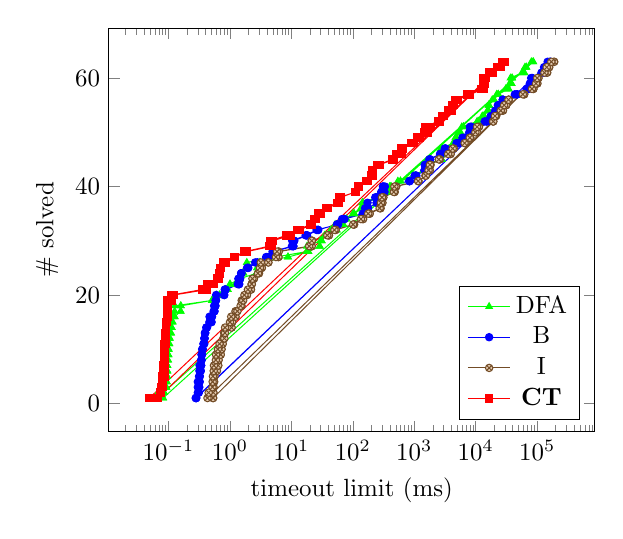
\begin{tikzpicture}[scale=0.9]
      \begin{axis}[
    xmode=log,
    every axis plot/.style={thin},
    xlabel={timeout limit (ms)},
    ylabel={\# solved},
    legend pos=south east
    % table/create on use/cumulative distribution/.style={
    %   create col/expr={\pgfmathaccuma + \thisrow{f(x)}}   
    % }
    ]
    \addplot 
    [mark=triangle*,
    mark size=1.5,
    mark options={solid},
    green] 
    coordinates {
    (0.082, 1)
(0.085, 2)
(0.092, 3)
(0.093, 4)
(0.095, 5)
(0.096, 6)
(0.096, 7)
(0.097, 8)
(0.099, 9)
(0.100, 10)
(0.101, 11)
(0.103, 12)
(0.110, 13)
(0.113, 14)
(0.117, 15)
(0.126, 16)
(0.158, 17)
(0.159, 18)
(0.512, 19)
(0.679, 20)
(0.837, 21)
(1.003, 22)
(1.452, 23)
(2.691, 24)
(2.775, 25)
(3.082, 26)
(8.824, 27)
(18.936, 28)
(28.930, 29)
(31.144, 30)
(36.765, 31)
(54.426, 32)
(70.085, 33)
(78.962, 34)
(105.003, 35)
(144.766, 36)
(145.095, 37)
(304.356, 38)
(354.576, 39)
(417.873, 40)
(596.434, 41)
(1054.559, 42)
(1409.747, 43)
(1550.990, 44)
(2795.949, 45)
(2856.575, 46)
(2905.908, 47)
(4426.888, 48)
(4837.998, 49)
(5613.862, 50)
(6339.689, 51)
(11098.021, 52)
(13598.524, 53)
(16105.137, 54)
(16456.706, 55)
(19834.691, 56)
(23268.929, 57)
(34232.672, 58)
(38227.578, 59)
(39121.745, 60)
(61565.556, 61)
(66501.499, 62)
(86189.149, 63)
(0.082, 1)
(0.085, 2)
(0.092, 3)
(0.093, 4)
(0.095, 5)
(0.096, 6)
(0.096, 7)
(0.097, 8)
(0.099, 9)
(0.100, 10)
(0.101, 11)
(0.103, 12)
(0.110, 13)
(0.113, 14)
(0.117, 15)
(0.126, 16)
(0.158, 17)
(0.159, 18)
(0.512, 19)
(0.679, 20)
(0.837, 21)
(1.003, 22)
(1.452, 23)
(2.691, 24)
(2.775, 25)
(3.082, 26)
(8.824, 27)
(18.936, 28)
(28.930, 29)
(31.144, 30)
(36.765, 31)
(54.426, 32)
(70.085, 33)
(78.962, 34)
(105.003, 35)
(144.766, 36)
(145.095, 37)
(304.356, 38)
(354.576, 39)
(417.873, 40)
(596.434, 41)
(1054.559, 42)
(1409.747, 43)
(1550.990, 44)
(2795.949, 45)
(2856.575, 46)
(2905.908, 47)
(4426.888, 48)
(4837.998, 49)
(5613.862, 50)
(6339.689, 51)
(11098.021, 52)
(13598.524, 53)
(16105.137, 54)
(16456.706, 55)
(19834.691, 56)
(23268.929, 57)
(34232.672, 58)
(38227.578, 59)
(39121.745, 60)
(61565.556, 61)
(66501.499, 62)
(86189.149, 63)
(0.066, 1)
(0.068, 2)
(0.091, 3)
(0.094, 4)
(0.095, 5)
(0.095, 6)
(0.095, 7)
(0.099, 8)
(0.100, 9)
(0.101, 10)
(0.104, 11)
(0.106, 12)
(0.107, 13)
(0.107, 14)
(0.112, 15)
(0.117, 16)
(0.126, 17)
(0.127, 18)
(0.516, 19)
(0.611, 20)
(0.929, 21)
(1.233, 22)
(1.405, 23)
(1.674, 24)
(1.808, 25)
(1.886, 26)
(5.602, 27)
(17.660, 28)
(18.013, 29)
(29.623, 30)
(34.824, 31)
(43.916, 32)
(51.570, 33)
(73.893, 34)
(100.339, 35)
(135.344, 36)
(142.453, 37)
(240.097, 38)
(280.974, 39)
(398.980, 40)
(541.521, 41)
(967.585, 42)
(1451.037, 43)
(1568.150, 44)
(2645.347, 45)
(2653.285, 46)
(2718.080, 47)
(4270.837, 48)
(4666.845, 49)
(5313.891, 50)
(5942.313, 51)
(10533.539, 52)
(12801.530, 53)
(15507.448, 54)
(16162.528, 55)
(18609.243, 56)
(21986.427, 57)
(30769.247, 58)
(35629.869, 59)
(36807.414, 60)
(56676.312, 61)
(63269.524, 62)
(80490.949, 63)
    };

    \addplot 
    [blue,
    mark=*,
    mark size=1.5,
    mark options={solid}]
    coordinates {
    (0.283, 1)
(0.311, 2)
(0.316, 3)
(0.321, 4)
(0.323, 5)
(0.335, 6)
(0.340, 7)
(0.345, 8)
(0.347, 9)
(0.360, 10)
(0.381, 11)
(0.386, 12)
(0.394, 13)
(0.415, 14)
(0.501, 15)
(0.510, 16)
(0.560, 17)
(0.580, 18)
(0.591, 19)
(0.807, 20)
(0.849, 21)
(1.412, 22)
(1.462, 23)
(1.537, 24)
(1.979, 25)
(2.792, 26)
(4.257, 27)
(5.214, 28)
(10.763, 29)
(11.117, 30)
(17.960, 31)
(27.243, 32)
(55.453, 33)
(72.889, 34)
(154.293, 35)
(175.823, 36)
(245.329, 37)
(245.445, 38)
(292.127, 39)
(310.830, 40)
(840.827, 41)
(1076.353, 42)
(1479.355, 43)
(1548.370, 44)
(1812.313, 45)
(2691.941, 46)
(3230.108, 47)
(5221.310, 48)
(6731.776, 49)
(8343.973, 50)
(8453.543, 51)
(15067.779, 52)
(19360.841, 53)
(22076.805, 54)
(23897.068, 55)
(27764.151, 56)
(47171.890, 57)
(71941.597, 58)
(78415.831, 59)
(82829.561, 60)
(130327.391, 61)
(134710.832, 62)
(162947.414, 63)
(0.283, 1)
(0.311, 2)
(0.316, 3)
(0.321, 4)
(0.323, 5)
(0.335, 6)
(0.340, 7)
(0.345, 8)
(0.347, 9)
(0.360, 10)
(0.381, 11)
(0.386, 12)
(0.394, 13)
(0.415, 14)
(0.501, 15)
(0.510, 16)
(0.560, 17)
(0.580, 18)
(0.591, 19)
(0.807, 20)
(0.849, 21)
(1.412, 22)
(1.462, 23)
(1.537, 24)
(1.979, 25)
(2.792, 26)
(4.257, 27)
(5.214, 28)
(10.763, 29)
(11.117, 30)
(17.960, 31)
(27.243, 32)
(55.453, 33)
(72.889, 34)
(154.293, 35)
(175.823, 36)
(245.329, 37)
(245.445, 38)
(292.127, 39)
(310.830, 40)
(840.827, 41)
(1076.353, 42)
(1479.355, 43)
(1548.370, 44)
(1812.313, 45)
(2691.941, 46)
(3230.108, 47)
(5221.310, 48)
(6731.776, 49)
(8343.973, 50)
(8453.543, 51)
(15067.779, 52)
(19360.841, 53)
(22076.805, 54)
(23897.068, 55)
(27764.151, 56)
(47171.890, 57)
(71941.597, 58)
(78415.831, 59)
(82829.561, 60)
(130327.391, 61)
(134710.832, 62)
(162947.414, 63)
(0.278, 1)
(0.301, 2)
(0.301, 3)
(0.301, 4)
(0.315, 5)
(0.320, 6)
(0.322, 7)
(0.341, 8)
(0.352, 9)
(0.354, 10)
(0.371, 11)
(0.387, 12)
(0.397, 13)
(0.424, 14)
(0.464, 15)
(0.467, 16)
(0.544, 17)
(0.555, 18)
(0.591, 19)
(0.598, 20)
(0.825, 21)
(1.345, 22)
(1.375, 23)
(1.523, 24)
(1.904, 25)
(2.581, 26)
(3.894, 27)
(4.948, 28)
(10.227, 29)
(10.343, 30)
(17.104, 31)
(25.747, 32)
(57.649, 33)
(66.990, 34)
(145.149, 35)
(158.730, 36)
(173.581, 37)
(232.098, 38)
(328.059, 39)
(332.837, 40)
(830.786, 41)
(1017.023, 42)
(1473.627, 43)
(1479.535, 44)
(1759.707, 45)
(2628.737, 46)
(3139.802, 47)
(4874.763, 48)
(6091.974, 49)
(7874.454, 50)
(8058.759, 51)
(13975.351, 52)
(17514.164, 53)
(20673.449, 54)
(22945.763, 55)
(27513.653, 56)
(43402.794, 57)
(67239.223, 58)
(76003.939, 59)
(79920.398, 60)
(117672.945, 61)
(129362.050, 62)
(148231.657, 63)
    };

    \addplot [brown!60!black,
    mark options={fill=brown!40},
    mark=otimes*,
    mark size=1.5]
    coordinates {
    (0.533, 1)
(0.538, 2)
(0.541, 3)
(0.553, 4)
(0.560, 5)
(0.614, 6)
(0.646, 7)
(0.654, 8)
(0.709, 9)
(0.730, 10)
(0.763, 11)
(0.786, 12)
(0.807, 13)
(1.064, 14)
(1.089, 15)
(1.233, 16)
(1.239, 17)
(1.539, 18)
(1.564, 19)
(1.894, 20)
(2.201, 21)
(2.267, 22)
(2.460, 23)
(2.973, 24)
(3.307, 25)
(4.220, 26)
(6.161, 27)
(6.216, 28)
(21.406, 29)
(21.706, 30)
(40.890, 31)
(52.574, 32)
(104.760, 33)
(146.690, 34)
(188.076, 35)
(282.436, 36)
(302.735, 37)
(313.414, 38)
(479.449, 39)
(507.178, 40)
(1169.855, 41)
(1526.330, 42)
(1793.206, 43)
(1835.741, 44)
(2601.589, 45)
(3905.199, 46)
(4380.029, 47)
(6841.344, 48)
(8153.461, 49)
(10568.256, 50)
(11292.264, 51)
(19221.124, 52)
(21430.002, 53)
(27742.165, 54)
(31405.082, 55)
(34438.370, 56)
(61507.382, 57)
(86746.039, 58)
(100544.177, 59)
(104826.284, 60)
(145237.900, 61)
(156735.930, 62)
(188815.099, 63)
(0.533, 1)
(0.538, 2)
(0.541, 3)
(0.553, 4)
(0.560, 5)
(0.614, 6)
(0.646, 7)
(0.654, 8)
(0.709, 9)
(0.730, 10)
(0.763, 11)
(0.786, 12)
(0.807, 13)
(1.064, 14)
(1.089, 15)
(1.233, 16)
(1.239, 17)
(1.539, 18)
(1.564, 19)
(1.894, 20)
(2.201, 21)
(2.267, 22)
(2.460, 23)
(2.973, 24)
(3.307, 25)
(4.220, 26)
(6.161, 27)
(6.216, 28)
(21.406, 29)
(21.706, 30)
(40.890, 31)
(52.574, 32)
(104.760, 33)
(146.690, 34)
(188.076, 35)
(282.436, 36)
(302.735, 37)
(313.414, 38)
(479.449, 39)
(507.178, 40)
(1169.855, 41)
(1526.330, 42)
(1793.206, 43)
(1835.741, 44)
(2601.589, 45)
(3905.199, 46)
(4380.029, 47)
(6841.344, 48)
(8153.461, 49)
(10568.256, 50)
(11292.264, 51)
(19221.124, 52)
(21430.002, 53)
(27742.165, 54)
(31405.082, 55)
(34438.370, 56)
(61507.382, 57)
(86746.039, 58)
(100544.177, 59)
(104826.284, 60)
(145237.900, 61)
(156735.930, 62)
(188815.099, 63)
(0.432, 1)
(0.451, 2)
(0.521, 3)
(0.524, 4)
(0.529, 5)
(0.545, 6)
(0.550, 7)
(0.591, 8)
(0.594, 9)
(0.638, 10)
(0.678, 11)
(0.813, 12)
(0.832, 13)
(0.835, 14)
(1.003, 15)
(1.050, 16)
(1.326, 17)
(1.493, 18)
(1.648, 19)
(1.725, 20)
(1.963, 21)
(2.268, 22)
(2.327, 23)
(2.862, 24)
(3.080, 25)
(3.185, 26)
(5.613, 27)
(5.857, 28)
(19.490, 29)
(21.493, 30)
(38.484, 31)
(50.269, 32)
(101.243, 33)
(135.636, 34)
(178.425, 35)
(273.453, 36)
(286.616, 37)
(298.204, 38)
(464.717, 39)
(475.543, 40)
(1157.973, 41)
(1543.458, 42)
(1709.910, 43)
(1800.555, 44)
(2510.186, 45)
(3565.914, 46)
(4214.736, 47)
(6597.529, 48)
(8011.713, 49)
(9883.265, 50)
(10530.998, 51)
(19314.981, 52)
(20605.964, 53)
(25567.274, 54)
(29024.888, 55)
(34130.201, 56)
(58493.658, 57)
(82449.996, 58)
(95806.320, 59)
(100158.601, 60)
(131283.508, 61)
(143158.851, 62)
(170170.634, 63)
    };

    \addplot 
    [red,
    mark size=1.5,
    mark=square*]
    coordinates {
    (0.049, 1)
(0.073, 2)
(0.082, 3)
(0.082, 4)
(0.086, 5)
(0.086, 6)
(0.086, 7)
(0.087, 8)
(0.088, 9)
(0.088, 10)
(0.089, 11)
(0.089, 12)
(0.090, 13)
(0.091, 14)
(0.093, 15)
(0.094, 16)
(0.095, 17)
(0.095, 18)
(0.096, 19)
(0.122, 20)
(0.425, 21)
(0.427, 22)
(0.657, 23)
(0.669, 24)
(0.716, 25)
(0.860, 26)
(1.221, 27)
(1.884, 28)
(4.877, 29)
(4.971, 30)
(9.723, 31)
(13.717, 32)
(21.682, 33)
(25.392, 34)
(30.293, 35)
(39.297, 36)
(58.995, 37)
(63.472, 38)
(109.895, 39)
(127.200, 40)
(175.921, 41)
(211.474, 42)
(211.537, 43)
(270.151, 44)
(468.503, 45)
(624.233, 46)
(650.780, 47)
(966.909, 48)
(1212.745, 49)
(1638.882, 50)
(1827.039, 51)
(2634.946, 52)
(2981.677, 53)
(4075.179, 54)
(4366.379, 55)
(5095.686, 56)
(8127.353, 57)
(13655.904, 58)
(14207.754, 59)
(14375.520, 60)
(18706.041, 61)
(25336.115, 62)
(30053.479, 63)
(0.049, 1)
(0.073, 2)
(0.082, 3)
(0.082, 4)
(0.086, 5)
(0.086, 6)
(0.086, 7)
(0.087, 8)
(0.088, 9)
(0.088, 10)
(0.089, 11)
(0.089, 12)
(0.090, 13)
(0.091, 14)
(0.093, 15)
(0.094, 16)
(0.095, 17)
(0.095, 18)
(0.096, 19)
(0.122, 20)
(0.425, 21)
(0.427, 22)
(0.657, 23)
(0.669, 24)
(0.716, 25)
(0.860, 26)
(1.221, 27)
(1.884, 28)
(4.877, 29)
(4.971, 30)
(9.723, 31)
(13.717, 32)
(21.682, 33)
(25.392, 34)
(30.293, 35)
(39.297, 36)
(58.995, 37)
(63.472, 38)
(109.895, 39)
(127.200, 40)
(175.921, 41)
(211.474, 42)
(211.537, 43)
(270.151, 44)
(468.503, 45)
(624.233, 46)
(650.780, 47)
(966.909, 48)
(1212.745, 49)
(1638.882, 50)
(1827.039, 51)
(2634.946, 52)
(2981.677, 53)
(4075.179, 54)
(4366.379, 55)
(5095.686, 56)
(8127.353, 57)
(13655.904, 58)
(14207.754, 59)
(14375.520, 60)
(18706.041, 61)
(25336.115, 62)
(30053.479, 63)
(0.068, 1)
(0.075, 2)
(0.075, 3)
(0.078, 4)
(0.080, 5)
(0.081, 6)
(0.083, 7)
(0.084, 8)
(0.084, 9)
(0.085, 10)
(0.086, 11)
(0.088, 12)
(0.089, 13)
(0.091, 14)
(0.094, 15)
(0.096, 16)
(0.096, 17)
(0.099, 18)
(0.112, 19)
(0.113, 20)
(0.354, 21)
(0.553, 22)
(0.617, 23)
(0.681, 24)
(0.689, 25)
(0.765, 26)
(1.168, 27)
(1.741, 28)
(4.369, 29)
(4.569, 30)
(8.310, 31)
(12.613, 32)
(20.407, 33)
(23.171, 34)
(27.733, 35)
(36.337, 36)
(54.814, 37)
(60.107, 38)
(112.995, 39)
(120.636, 40)
(163.060, 41)
(197.055, 42)
(209.187, 43)
(253.124, 44)
(443.651, 45)
(513.516, 46)
(605.313, 47)
(897.353, 48)
(1100.299, 49)
(1456.227, 50)
(1493.212, 51)
(2413.262, 52)
(2823.822, 53)
(3625.762, 54)
(4106.303, 55)
(4711.728, 56)
(7250.264, 57)
(12475.854, 58)
(13043.974, 59)
(13302.789, 60)
(16441.540, 61)
(22312.608, 62)
(26520.260, 63)
    };
    \legend{DFA,B,I,\textbf{CT}}
  \end{axis}

    \end{tikzpicture}
    \vfill
    \caption{\textbf{Crosswords LexVG}.}
    \vspace{\baselineskip}
  \end{minipage}\qquad
\end{figure}

\clearpage

\begin{figure}
  \begin{minipage}[b][10cm][s]{0.45\textwidth}
    \centering
    \vfill
    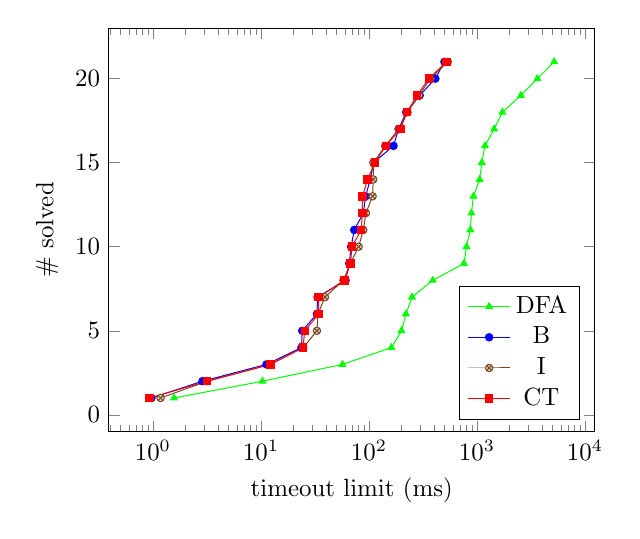
\begin{tikzpicture}[scale=0.9]
      \begin{axis}[
    xmode=log,
    every axis plot/.style={thin},
    xlabel={timeout limit (ms)},
    ylabel={\# solved},
    legend pos=south east
    % table/create on use/cumulative distribution/.style={
    %   create col/expr={\pgfmathaccuma + \thisrow{f(x)}}   
    % }
    ]
    \addplot 
    [mark=triangle*,
    mark size=1.5,
    mark options={solid},
    green] 
    coordinates {
(1.569, 1)
(10.341, 2)
(56.930, 3)
(161.466, 4)
(200.271, 5)
(220.150, 6)
(250.496, 7)
(389.479, 8)
(757.830, 9)
(800.580, 10)
(868.873, 11)
(888.415, 12)
(928.329, 13)
(1059.826, 14)
(1108.592, 15)
(1186.171, 16)
(1442.143, 17)
(1718.117, 18)
(2549.019, 19)
(3626.036, 20)
(5178.601, 21)
    };

    \addplot 
    [blue,
    mark=*,
    mark size=1.5,
    mark options={solid}]
    coordinates {
(0.969, 1)
(2.881, 2)
(11.268, 3)
(23.734, 4)
(24.138, 5)
(33.016, 6)
(33.480, 7)
(60.819, 8)
(65.730, 9)
(68.464, 10)
(73.136, 11)
(88.944, 12)
(92.941, 13)
(103.030, 14)
(110.307, 15)
(168.815, 16)
(188.304, 17)
(221.341, 18)
(295.291, 19)
(412.154, 20)
(499.695, 21)
    };

    \addplot [brown!60!black,
    mark options={fill=brown!40},
    mark=otimes*,
    mark size=1.5]
    coordinates {
(1.178, 1)
(3.182, 2)
(12.190, 3)
(24.682, 4)
(33.012, 5)
(33.778, 6)
(39.197, 7)
(58.045, 8)
(67.182, 9)
(80.311, 10)
(88.742, 11)
(93.862, 12)
(108.193, 13)
(109.575, 14)
(110.207, 15)
(141.416, 16)
(189.383, 17)
(227.490, 18)
(289.981, 19)
(370.487, 20)
(537.222, 21)
    };

    \addplot 
    [red,
    mark size=1.5,
    mark=square*]
    coordinates {
(0.929, 1)
(3.171, 2)
(12.289, 3)
(24.504, 4)
(25.467, 5)
(34.223, 6)
(34.294, 7)
(59.192, 8)
(67.660, 9)
(69.445, 10)
(84.905, 11)
(86.923, 12)
(87.166, 13)
(97.317, 14)
(113.314, 15)
(143.394, 16)
(195.333, 17)
(225.252, 18)
(279.125, 19)
(358.324, 20)
(525.028, 21)
    };
    \legend{DFA,B,I,CT}
  \end{axis}

    \end{tikzpicture}
    \vfill
    \caption{\textbf{Crosswords Wordspuzzle}.}
    \vspace{\baselineskip}
  \end{minipage}\qquad
  \begin{minipage}[b][10cm][s]{0.45\textwidth}
    \centering
    \vfill
    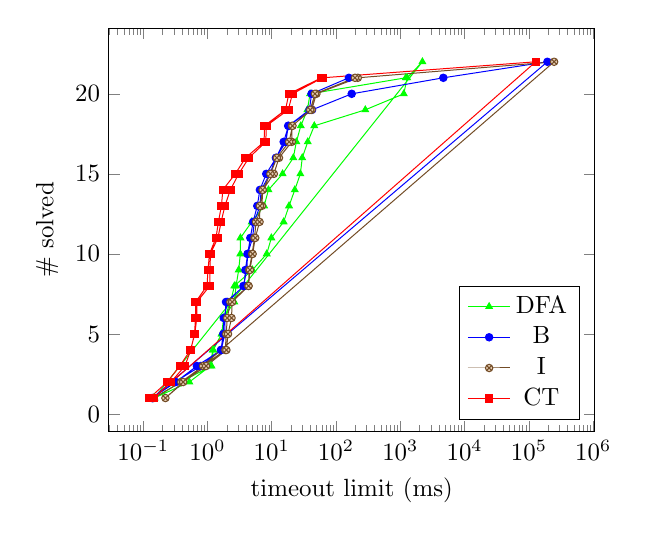
\begin{tikzpicture}[scale=0.9]
      \begin{axis}[
    xmode=log,
    every axis plot/.style={thin},
    xlabel={timeout limit (ms)},
    ylabel={\# solved},
    legend pos=south east
    % table/create on use/cumulative distribution/.style={
    %   create col/expr={\pgfmathaccuma + \thisrow{f(x)}}   
    % }
    ]
    \addplot 
    [mark=triangle*,
    mark size=1.5,
    mark options={solid},
    green] 
    coordinates {
    (0.150, 1)
(0.382, 2)
(1.156, 3)
(1.231, 4)
(1.662, 5)
(1.826, 6)
(2.291, 7)
(2.622, 8)
(5.011, 9)
(8.353, 10)
(9.860, 11)
(15.302, 12)
(18.579, 13)
(22.834, 14)
(27.862, 15)
(29.816, 16)
(36.345, 17)
(45.878, 18)
(285.224, 19)
(1131.791, 20)
(1278.079, 21)
(2204.696, 22)
(0.149, 1)
(0.523, 2)
(1.108, 3)
(1.209, 4)
(1.664, 5)
(1.784, 6)
(2.615, 7)
(2.780, 8)
(3.064, 9)
(3.247, 10)
(3.259, 11)
(4.882, 12)
(7.608, 13)
(8.891, 14)
(14.751, 15)
(21.638, 16)
(24.155, 17)
(28.300, 18)
(35.883, 19)
(39.440, 20)
(1216.894, 21)
    };

    \addplot 
    [blue,
    mark=*,
    mark size=1.5,
    mark options={solid}]
    coordinates {
    (0.138, 1)
(0.311, 2)
(0.790, 3)
(1.624, 4)
(1.760, 5)
(1.791, 6)
(2.063, 7)
(3.631, 8)
(4.094, 9)
(4.213, 10)
(5.035, 11)
(5.357, 12)
(6.556, 13)
(6.847, 14)
(9.371, 15)
(11.612, 16)
(16.633, 17)
(18.028, 18)
(42.410, 19)
(175.300, 20)
(4664.842, 21)
(193998.166, 22)
(0.139, 1)
(0.322, 2)
(0.685, 3)
(1.637, 4)
(1.865, 5)
(1.874, 6)
(1.944, 7)
(3.723, 8)
(3.895, 9)
(4.222, 10)
(4.642, 11)
(5.131, 12)
(5.954, 13)
(6.538, 14)
(8.208, 15)
(11.710, 16)
(15.325, 17)
(18.221, 18)
(38.590, 19)
(41.567, 20)
(158.242, 21)
    };

    \addplot [brown!60!black,
    mark options={fill=brown!40},
    mark=otimes*,
    mark size=1.5]
    coordinates {
    (0.146, 1)
(0.391, 2)
(0.855, 3)
(1.897, 4)
(1.958, 5)
(2.033, 6)
(2.272, 7)
(4.342, 8)
(4.459, 9)
(4.946, 10)
(5.389, 11)
(5.697, 12)
(7.018, 13)
(7.259, 14)
(10.784, 15)
(12.976, 16)
(20.478, 17)
(20.679, 18)
(41.775, 19)
(49.515, 20)
(218.327, 21)
(246737.472, 22)
(0.222, 1)
(0.419, 2)
(0.952, 3)
(1.971, 4)
(2.089, 5)
(2.368, 6)
(2.424, 7)
(4.359, 8)
(4.581, 9)
(5.042, 10)
(5.547, 11)
(6.463, 12)
(6.545, 13)
(7.219, 14)
(9.536, 15)
(11.997, 16)
(18.667, 17)
(21.020, 18)
(39.703, 19)
(47.031, 20)
(197.000, 21)
    };

    \addplot 
    [red,
    mark size=1.5,
    mark=square*]
    coordinates {
    (0.125, 1)
(0.237, 2)
(0.372, 3)
(0.544, 4)
(0.636, 5)
(0.682, 6)
(0.685, 7)
(1.085, 8)
(1.099, 9)
(1.110, 10)
(1.455, 11)
(1.631, 12)
(1.870, 13)
(2.270, 14)
(3.062, 15)
(4.409, 16)
(8.078, 17)
(8.255, 18)
(18.086, 19)
(20.971, 20)
(61.702, 21)
(127890.223, 22)
(0.145, 1)
(0.271, 2)
(0.446, 3)
(0.550, 4)
(0.628, 5)
(0.653, 6)
(0.654, 7)
(0.983, 8)
(1.021, 9)
(1.074, 10)
(1.357, 11)
(1.482, 12)
(1.649, 13)
(1.736, 14)
(2.708, 15)
(3.908, 16)
(7.615, 17)
(7.716, 18)
(16.348, 19)
(18.448, 20)
(59.463, 21)
    };
    \legend{DFA,B,I,CT}
  \end{axis}

    \end{tikzpicture}
    \vfill
    \caption{\textbf{Crosswords Wordspuzzle}.}
    \vspace{\baselineskip}
  \end{minipage}\qquad
\end{figure}

\begin{figure}
    \begin{minipage}[b][10cm][s]{0.45\textwidth}
    \centering
    \vfill
    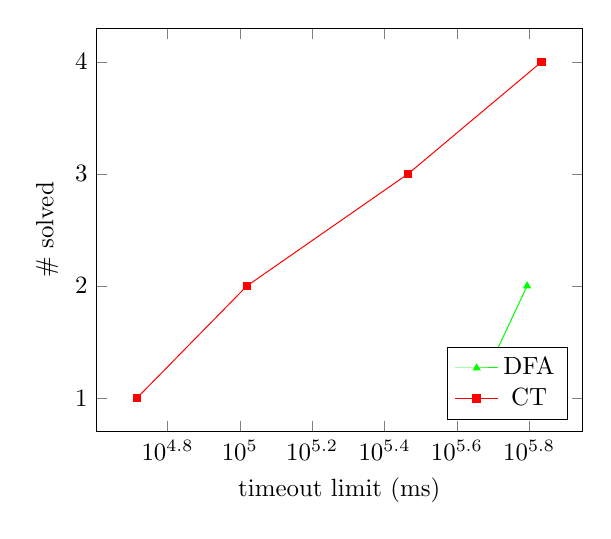
\begin{tikzpicture}[scale=0.9]
      \begin{axis}[
    xmode=log,
    every axis plot/.style={thin},
    xlabel={timeout limit (ms)},
    ylabel={\# solved},
    legend pos=south east
    % table/create on use/cumulative distribution/.style={
    %   create col/expr={\pgfmathaccuma + \thisrow{f(x)}}   
    % }
    ]
    \addplot 
    [mark=triangle*,
    mark size=1.5,
    mark options={solid},
    green] 
    coordinates {
    (445273.296, 1)
(622414.790, 2)
% (1031281.648, 3)
% (1073752.509, 4)
% (1077338.303, 5)
% (1078117.880, 6)
% (1078636.961, 7)
% (1079178.894, 8)
% (1079839.216, 9)
% (1080840.349, 10)
% (1082059.397, 11)
% (1083648.155, 12)
% (1083902.339, 13)
% (1083988.269, 14)
% (1084069.534, 15)
% (1084396.676, 16)
% (1085666.524, 17)
% (1089495.967, 18)
% (1091132.921, 19)
% (1091433.340, 20)
% (1092057.252, 21)
% (1093916.092, 22)
% (1094177.223, 23)
% (1114453.122, 24)
% (1115067.373, 25)
    };

%     \addplot 
%     [blue,
%     mark=*,
%     mark size=1.5,
%     mark options={solid}]
%     coordinates {
%     (1004672.786, 1)
% (1004695.224, 2)
% (1004696.645, 3)
% (1004718.463, 4)
% (1004738.023, 5)
% (1004743.967, 6)
% (1004751.151, 7)
% (1004765.567, 8)
% (1004781.515, 9)
% (1004797.803, 10)
% (1004816.640, 11)
% (1004820.096, 12)
% (1004835.673, 13)
% (1004864.792, 14)
% (1004881.537, 15)
% (1004913.526, 16)
% (1004920.059, 17)
% (1004929.625, 18)
% (1004958.448, 19)
% (1004996.508, 20)
% (1005007.752, 21)
% (1005029.139, 22)
% (1005067.535, 23)
% (1005104.606, 24)
% (1040982.750, 25)
%     };

%     \addplot [brown!60!black,
%     mark options={fill=brown!40},
%     mark=otimes*,
%     mark size=1.5]
%     coordinates {
%     (1004653.569, 1)
% (1004695.464, 2)
% (1004715.665, 3)
% (1004725.629, 4)
% (1004729.598, 5)
% (1004736.757, 6)
% (1004768.906, 7)
% (1004774.513, 8)
% (1004800.095, 9)
% (1004877.671, 10)
% (1004885.444, 11)
% (1004924.289, 12)
% (1004954.273, 13)
% (1004976.220, 14)
% (1005012.748, 15)
% (1005016.479, 16)
% (1005025.501, 17)
% (1005059.309, 18)
% (1005081.774, 19)
% (1005131.686, 20)
% (1005177.022, 21)
% (1005199.107, 22)
% (1005247.884, 23)
% (1005272.462, 24)
% (1103825.908, 25)
%     };

    \addplot 
    [red,
    mark size=1.5,
    mark=square*]
    coordinates {
    (51933.780, 1)
(104573.439, 2)
(291800.057, 3)
(683133.039, 4)
% (1006259.610, 5)
% (1006270.822, 6)
% (1006282.419, 7)
% (1006303.104, 8)
% (1006319.339, 9)
% (1006423.422, 10)
% (1006449.607, 11)
% (1006459.928, 12)
% (1006499.500, 13)
% (1006510.783, 14)
% (1006510.952, 15)
% (1006511.373, 16)
% (1006567.036, 17)
% (1006579.356, 18)
% (1006588.135, 19)
% (1006591.883, 20)
% (1006659.196, 21)
% (1006817.280, 22)
% (1006986.645, 23)
% (1012355.582, 24)
% (1025624.781, 25)
    };
    \legend{DFA,CT}
  \end{axis}

    \end{tikzpicture}
    \vfill
    \caption{\textbf{MDD 05}.}
    \vspace{\baselineskip}
  \end{minipage}\qquad
    \begin{minipage}[b][10cm][s]{0.45\textwidth}
    \centering
    \vfill
    \begin{tikzpicture}[scale=0.9]
      \begin{axis}[
    xmode=log,
    every axis plot/.style={thin},
    xlabel={timeout limit (ms)},
    ylabel={\% solved},
    legend pos=south east,
    cycle list/Set1-6,
            % define fill color for the marker
            mark list fill={.!75!white},
            mark options={solid},
            cycle multiindex* list={
                Set1-6
                    \nextlist
                [3 of]linestyles
                    \nextlist
                very thick
                \nextlist
                mark=o,
                mark=*,
                mark=square,
                mark=triangle,
                mark=+
            },
    ]

    \addplot
    coordinates {
      (34430, 4)
      (71030, 8)
      (200120, 12)
      (524830, 16)
      (901810, 20)
      (982210, 24)
      
    };
    \addplot
    coordinates {
      (1000010, 96)
      
    };
    \addplot
    coordinates {
      (1000010, 100)
      
    };
    \addplot
    coordinates {
      (25840, 4)
      (55070, 8)
      (183300, 12)
      (394620, 16)
      (673890, 20)
      (710840, 24)
      (782830, 29)
      (918440, 32)
      (974790, 36)
      
    };
    

    \legend{ DFA, B, I, \textbf{CT} }
  \end{axis}

    \end{tikzpicture}
    \vfill
    \caption{\textbf{MDD 05}.}
    \vspace{\baselineskip}
  \end{minipage}\qquad
\end{figure}

\clearpage

\begin{figure}
  \begin{minipage}[b][10cm][s]{0.45\textwidth}
    \centering
    \vfill
    \begin{tikzpicture}[scale=0.9]
      %\begin{axis}[
    xmode=log,
    every axis plot/.style={thin},
    xlabel={timeout limit (ms)},
    ylabel={\% solved},
    legend pos=south east,
    cycle list/Set1-6,
            % define fill color for the marker
            mark list fill={.!75!white},
            mark options={solid},
            cycle multiindex* list={
                Set1-6
                    \nextlist
                [3 of]linestyles
                    \nextlist
                very thick
                \nextlist
                mark=o,
                mark=*,
                mark=square,
                mark=triangle,
                mark=+
            },
    ]

    \addplot
    coordinates {
      (1075850, 12)
      
    };
    \addplot
    coordinates {
      (1005290, 23)
      
    };
    \addplot
    coordinates {
      (1005260, 12)
      
    };
    \addplot
    coordinates {
      (1005430, 12)
      
    };
    

    \legend{ DFA, B, I, \textbf{CT} }
  \end{axis}

    \end{tikzpicture}
    \vfill
    \caption{\textbf{MDD 07}.}
    \vspace{\baselineskip}
  \end{minipage}\qquad
    \begin{minipage}[b][10cm][s]{0.45\textwidth}
    \centering
    \vfill
    \begin{tikzpicture}[scale=0.9]
     % \begin{axis}[
    xmode=log,
    every axis plot/.style={thin},
    xlabel={timeout limit (ms)},
    ylabel={\# solved},
    legend pos=south east
    % table/create on use/cumulative distribution/.style={
    %   create col/expr={\pgfmathaccuma + \thisrow{f(x)}}   
    % }
    ]
    \addplot 
    [mark=triangle*,
    mark size=1.5,
    mark options={solid},
    green] 
    coordinates {
    (8143.453, 1)
(28227.868, 2)
(30184.398, 3)
(39636.695, 4)
(40458.753, 5)
(56228.579, 6)
(66820.027, 7)
(79866.961, 8)
(245383.866, 9)
    };

%     \addplot 
%     [blue,
%     mark=*,
%     mark size=1.5,
%     mark options={solid}]
%     coordinates {
%     (1000001.471, 1)
% (1000001.544, 2)
% (1000002.625, 3)
% (1000002.721, 4)
% (1000002.899, 5)
% (1000003.208, 6)
% (1000004.208, 7)
% (1000004.650, 8)
% (1000005.052, 9)
%     };

%     \addplot [brown!60!black,
%     mark options={fill=brown!40},
%     mark=otimes*,
%     mark size=1.5]
%     coordinates {
%     (1000000.498, 1)
% (1000000.780, 2)
% (1000000.821, 3)
% (1000001.078, 4)
% (1000001.299, 5)
% (1000001.505, 6)
% (1000002.168, 7)
% (1000004.073, 8)
% (1000008.854, 9)
%     };

%     \addplot 
%     [red,
%     mark size=1.5,
%     mark=square*]
%     coordinates {
%     (1000000.160, 1)
% (1000000.224, 2)
% (1000000.247, 3)
% (1000000.259, 4)
% (1000000.300, 5)
% (1000000.307, 6)
% (1000000.343, 7)
% (1000000.404, 8)
% (1000000.445, 9)
%     };
    \legend{DFA}
  \end{axis}

    \end{tikzpicture}
    \vfill
    \caption{\textbf{MDD 07}.}
    \vspace{\baselineskip}
  \end{minipage}\qquad
\end{figure}

\begin{figure}
  \begin{minipage}[b][10cm][s]{.45\textwidth}
    \centering
    \vfill
    \begin{tikzpicture}[scale=0.9]
%      \begin{axis}[
    xmode=log,
    every axis plot/.style={thin},
    xlabel={timeout limit (ms)},
    ylabel={\# solved},
    legend pos=south east
    % table/create on use/cumulative distribution/.style={
    %   create col/expr={\pgfmathaccuma + \thisrow{f(x)}}   
    % }
    ]
    \addplot 
    [mark=triangle*,
    mark size=1.5,
    mark options={solid},
    green] 
    coordinates {
    (76933.510, 1)
(78294.653, 2)
(83021.260, 3)
(83759.037, 4)
(84554.991, 5)
(85749.793, 6)
(87036.829, 7)
% (1199058.340, 8)
% (2881069.118, 9)
% (2938114.681, 10)
    };

%     \addplot 
%     [blue,
%     mark=*,
%     mark size=1.5,
%     mark options={solid}]
%     coordinates {
%     (1004711.558, 1)
% (1004853.521, 2)
% (1004873.643, 3)
% (1004892.668, 4)
% (1004916.234, 5)
% (1004930.276, 6)
% (1005198.940, 7)
% (1005342.500, 8)
% (1005648.193, 9)
% (1013663.806, 10)
%     };

%     \addplot [brown!60!black,
%     mark options={fill=brown!40},
%     mark=otimes*,
%     mark size=1.5]
%     coordinates {
%     (1004824.935, 1)
% (1004877.779, 2)
% (1004894.573, 3)
% (1004895.754, 4)
% (1004901.792, 5)
% (1004950.617, 6)
% (1005091.313, 7)
% (1005607.079, 8)
% (1026143.909, 9)
% (1491889.745, 10)
%     };

%     \addplot 
%     [red,
%     mark size=1.5,
%     mark=square*]
%     coordinates {
%     (1006452.964, 1)
% (1006494.239, 2)
% (1006495.989, 3)
% (1006530.881, 4)
% (1006640.811, 5)
% (1007100.106, 6)
% (1007189.809, 7)
% (1016125.780, 8)
% (1038915.096, 9)
% (1402042.841, 10)
%     };
    \legend{DFA}
  \end{axis}

    \end{tikzpicture}
    \vfill
    \caption{\textbf{MDD 09}.}
    \vspace{\baselineskip}
  \end{minipage}\qquad
  \begin{minipage}[b][10cm][s]{.45\textwidth}
    \centering
    \vfill
    \begin{tikzpicture}[scale=0.9]
 %     \begin{axis}[
    xmode=log,
    every axis plot/.style={thin},
    xlabel={timeout limit (ms)},
    ylabel={\# solved},
    legend pos=south east
    % table/create on use/cumulative distribution/.style={
    %   create col/expr={\pgfmathaccuma + \thisrow{f(x)}}   
    % }
    ]
    \addplot 
    [mark=triangle*,
    mark size=1.5,
    mark options={solid},
    green] 
    coordinates {
    (57.443, 1)
(69.762, 2)
(71.061, 3)
(91.280, 4)
(104.926, 5)
(164.083, 6)
(170.756, 7)
(180.872, 8)
(290.808, 9)
(20087.742, 10)
    };

%     \addplot 
%     [blue,
%     mark=*,
%     mark size=1.5,
%     mark options={solid}]
%     coordinates {
%     (1000001.184, 1)
% (1000001.366, 2)
% (1000001.371, 3)
% (1000001.512, 4)
% (1000001.799, 5)
% (1000002.918, 6)
% (1000004.281, 7)
% (1000005.887, 8)
% (1000008.173, 9)
% (1023550.411, 10)
%     };

%     \addplot [brown!60!black,
%     mark options={fill=brown!40},
%     mark=otimes*,
%     mark size=1.5]
%     coordinates {
%     (1000000.325, 1)
% (1000000.450, 2)
% (1000000.494, 3)
% (1000002.853, 4)
% (1000002.991, 5)
% (1000004.673, 6)
% (1000004.785, 7)
% (1000005.423, 8)
% (1021239.731, 9)
% (1046597.832, 10)
%     };

%     \addplot 
%     [red,
%     mark size=1.5,
%     mark=square*]
%     coordinates {
%     (1000000.183, 1)
% (1000000.183, 2)
% (1000000.278, 3)
% (1000000.320, 4)
% (1000000.424, 5)
% (1000000.441, 6)
% (1000000.643, 7)
% (1032144.225, 8)
% (1034410.530, 9)
% (1050562.565, 10)
%     };
    \legend{DFA}
  \end{axis}

    \end{tikzpicture}
    \vfill
    \caption{\textbf{MDD 09}.}
    \vspace{\baselineskip}
  \end{minipage}\qquad
\end{figure}

\clearpage

\begin{figure}
  \begin{minipage}[b][10cm][s]{0.45\textwidth}
    \centering
    \vfill
    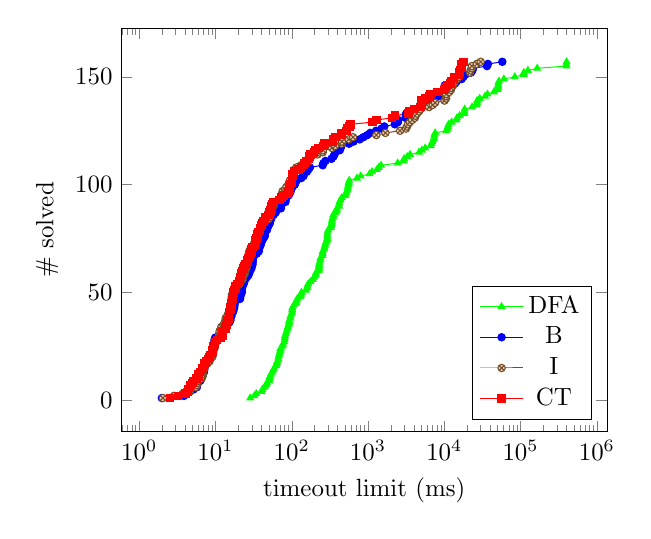
\begin{tikzpicture}[scale=0.9]
      \begin{axis}[
    xmode=log,
    every axis plot/.style={thin},
    xlabel={timeout limit (ms)},
    ylabel={\# solved},
    legend pos=south east
    % table/create on use/cumulative distribution/.style={
    %   create col/expr={\pgfmathaccuma + \thisrow{f(x)}}   
    % }
    ]
    \addplot 
    [mark=triangle*,
    mark size=1.5,
    mark options={solid},
    green] 
    coordinates {
    (28.479, 1)
(32.259, 2)
(34.184, 3)
(40.176, 4)
(41.117, 5)
(44.220, 6)
(46.524, 7)
(47.119, 8)
(50.594, 9)
(51.185, 10)
(51.683, 11)
(53.094, 12)
(55.381, 13)
(57.551, 14)
(58.822, 15)
(62.806, 16)
(64.164, 17)
(64.612, 18)
(66.816, 19)
(66.879, 20)
(68.064, 21)
(69.387, 22)
(70.958, 23)
(71.154, 24)
(74.896, 25)
(76.696, 26)
(79.628, 27)
(80.614, 28)
(80.994, 29)
(81.915, 30)
(83.799, 31)
(85.498, 32)
(87.376, 33)
(88.955, 34)
(90.775, 35)
(92.387, 36)
(92.399, 37)
(95.672, 38)
(96.038, 39)
(99.560, 40)
(101.063, 41)
(101.351, 42)
(102.343, 43)
(105.757, 44)
(114.544, 45)
(115.689, 46)
(117.793, 47)
(129.374, 48)
(131.156, 49)
(134.382, 50)
(152.723, 51)
(159.993, 52)
(160.432, 53)
(164.374, 54)
(176.218, 55)
(188.673, 56)
(197.819, 57)
(205.739, 58)
(207.344, 59)
(226.014, 60)
(227.529, 61)
(227.659, 62)
(227.801, 63)
(232.632, 64)
(236.122, 65)
(237.853, 66)
(253.358, 67)
(253.590, 68)
(254.330, 69)
(266.274, 70)
(268.730, 71)
(273.463, 72)
(277.735, 73)
(288.026, 74)
(291.548, 75)
(292.756, 76)
(293.227, 77)
(294.410, 78)
(300.709, 79)
(327.569, 80)
(332.541, 81)
(333.924, 82)
(334.411, 83)
(339.586, 84)
(348.199, 85)
(349.532, 86)
(371.373, 87)
(386.701, 88)
(390.963, 89)
(418.408, 90)
(418.695, 91)
(422.230, 92)
(437.503, 93)
(453.861, 94)
(502.971, 95)
(520.108, 96)
(527.304, 97)
(542.192, 98)
(544.013, 99)
(554.465, 100)
(558.086, 101)
(567.256, 102)
(715.556, 103)
(800.577, 104)
(1046.040, 105)
(1129.254, 106)
(1306.675, 107)
(1383.006, 108)
(1479.749, 109)
(2448.671, 110)
(2930.847, 111)
(2965.572, 112)
(3260.970, 113)
(3556.870, 114)
(4656.549, 115)
(5078.367, 116)
(5623.653, 117)
(6659.340, 118)
(6784.312, 119)
(6973.103, 120)
(7329.557, 121)
(7359.121, 122)
(7396.106, 123)
(7576.040, 124)
(10610.895, 125)
(10922.259, 126)
(11159.351, 127)
(11396.117, 128)
(12483.028, 129)
(14419.922, 130)
(14676.118, 131)
(15906.106, 132)
(18283.308, 133)
(18442.544, 134)
(18470.312, 135)
(23102.428, 136)
(26464.714, 137)
(26805.377, 138)
(26954.579, 139)
(29112.162, 140)
(34228.839, 141)
(36846.271, 142)
(44695.427, 143)
(50105.717, 144)
(50810.695, 145)
(50811.889, 146)
(51055.360, 147)
(51994.297, 148)
(60294.547, 149)
(83881.093, 150)
(110031.542, 151)
(110303.654, 152)
(124680.954, 153)
(164840.449, 154)
(398572.615, 155)
(398573.318, 156)
(401037.607, 157)
    };

    \addplot 
    [blue,
    mark=*,
    mark size=1.5,
    mark options={solid}]
    coordinates {
    (1.981, 1)
(3.865, 2)
(4.064, 3)
(4.147, 4)
(5.164, 5)
(5.702, 6)
(5.759, 7)
(5.839, 8)
(6.320, 9)
(6.503, 10)
(6.645, 11)
(6.804, 12)
(7.058, 13)
(7.115, 14)
(7.149, 15)
(7.349, 16)
(7.424, 17)
(7.744, 18)
(8.081, 19)
(8.255, 20)
(9.006, 21)
(9.029, 22)
(9.159, 23)
(9.557, 24)
(9.613, 25)
(9.675, 26)
(9.691, 27)
(9.705, 28)
(9.922, 29)
(11.049, 30)
(11.959, 31)
(12.363, 32)
(13.100, 33)
(13.492, 34)
(14.116, 35)
(15.142, 36)
(15.661, 37)
(15.767, 38)
(16.210, 39)
(16.247, 40)
(17.023, 41)
(17.310, 42)
(17.589, 43)
(17.712, 44)
(17.876, 45)
(18.383, 46)
(20.996, 47)
(21.124, 48)
(21.524, 49)
(22.126, 50)
(22.138, 51)
(22.244, 52)
(22.755, 53)
(23.472, 54)
(23.827, 55)
(24.361, 56)
(25.737, 57)
(27.024, 58)
(27.729, 59)
(28.322, 60)
(29.453, 61)
(30.020, 62)
(30.589, 63)
(30.689, 64)
(30.830, 65)
(31.200, 66)
(31.809, 67)
(34.778, 68)
(36.914, 69)
(36.958, 70)
(38.037, 71)
(39.151, 72)
(39.381, 73)
(40.922, 74)
(42.232, 75)
(44.223, 76)
(44.334, 77)
(44.614, 78)
(47.327, 79)
(47.856, 80)
(49.569, 81)
(51.504, 82)
(51.951, 83)
(53.451, 84)
(54.347, 85)
(57.828, 86)
(61.396, 87)
(63.159, 88)
(72.148, 89)
(72.466, 90)
(72.988, 91)
(82.727, 92)
(83.052, 93)
(85.267, 94)
(91.016, 95)
(94.242, 96)
(97.150, 97)
(97.576, 98)
(102.403, 99)
(109.460, 100)
(112.204, 101)
(115.663, 102)
(132.942, 103)
(142.599, 104)
(142.756, 105)
(158.121, 106)
(164.564, 107)
(173.027, 108)
(254.761, 109)
(260.341, 110)
(276.465, 111)
(331.631, 112)
(352.139, 113)
(362.559, 114)
(375.144, 115)
(427.109, 116)
(436.286, 117)
(447.651, 118)
(565.156, 119)
(646.826, 120)
(776.447, 121)
(868.556, 122)
(978.473, 123)
(1068.681, 124)
(1274.319, 125)
(1503.918, 126)
(1634.250, 127)
(2243.783, 128)
(2467.649, 129)
(2483.835, 130)
(3099.528, 131)
(3157.027, 132)
(3161.783, 133)
(3741.648, 134)
(3951.777, 135)
(5102.101, 136)
(5232.868, 137)
(5786.206, 138)
(6318.847, 139)
(7243.252, 140)
(8487.686, 141)
(9904.149, 142)
(10127.961, 143)
(10128.039, 144)
(10128.112, 145)
(10128.150, 146)
(13891.478, 147)
(14623.462, 148)
(16877.665, 149)
(17802.422, 150)
(18785.664, 151)
(22435.458, 152)
(23340.568, 153)
(23707.641, 154)
(36289.195, 155)
(37329.808, 156)
(57612.194, 157)
    };

    \addplot [brown!60!black,
    mark options={fill=brown!40},
    mark=otimes*,
    mark size=1.5]
    coordinates {
    (2.040, 1)
(2.855, 2)
(3.719, 3)
(4.632, 4)
(4.641, 5)
(5.533, 6)
(5.714, 7)
(5.787, 8)
(5.857, 9)
(6.577, 10)
(6.773, 11)
(6.786, 12)
(6.845, 13)
(7.010, 14)
(7.176, 15)
(7.222, 16)
(7.831, 17)
(8.350, 18)
(8.396, 19)
(9.065, 20)
(9.266, 21)
(9.307, 22)
(9.310, 23)
(9.701, 24)
(9.813, 25)
(9.942, 26)
(9.968, 27)
(10.442, 28)
(10.956, 29)
(11.109, 30)
(11.272, 31)
(11.322, 32)
(11.721, 33)
(11.918, 34)
(12.829, 35)
(13.226, 36)
(13.534, 37)
(13.610, 38)
(14.211, 39)
(14.646, 40)
(15.410, 41)
(15.583, 42)
(15.762, 43)
(15.958, 44)
(15.963, 45)
(16.254, 46)
(16.279, 47)
(16.369, 48)
(16.443, 49)
(17.092, 50)
(17.486, 51)
(18.263, 52)
(19.356, 53)
(20.741, 54)
(21.061, 55)
(22.659, 56)
(22.736, 57)
(23.631, 58)
(24.292, 59)
(24.320, 60)
(25.417, 61)
(25.501, 62)
(25.852, 63)
(26.675, 64)
(26.775, 65)
(26.937, 66)
(27.206, 67)
(27.302, 68)
(27.716, 69)
(28.500, 70)
(30.188, 71)
(31.872, 72)
(32.316, 73)
(33.242, 74)
(35.322, 75)
(35.465, 76)
(35.935, 77)
(36.585, 78)
(37.473, 79)
(39.837, 80)
(41.395, 81)
(41.916, 82)
(43.633, 83)
(49.626, 84)
(51.364, 85)
(51.918, 86)
(54.007, 87)
(54.632, 88)
(54.830, 89)
(57.738, 90)
(57.962, 91)
(59.061, 92)
(66.911, 93)
(72.484, 94)
(73.188, 95)
(75.152, 96)
(76.043, 97)
(82.614, 98)
(85.390, 99)
(92.294, 100)
(92.310, 101)
(94.799, 102)
(100.399, 103)
(103.386, 104)
(104.357, 105)
(107.466, 106)
(108.809, 107)
(115.076, 108)
(132.377, 109)
(150.485, 110)
(155.998, 111)
(165.401, 112)
(168.692, 113)
(217.693, 114)
(254.736, 115)
(256.005, 116)
(335.905, 117)
(372.441, 118)
(450.372, 119)
(454.066, 120)
(558.160, 121)
(636.164, 122)
(1284.240, 123)
(1689.710, 124)
(2626.867, 125)
(3141.959, 126)
(3250.413, 127)
(3340.003, 128)
(3529.547, 129)
(3796.970, 130)
(4107.852, 131)
(4203.355, 132)
(4401.731, 133)
(4666.155, 134)
(4868.455, 135)
(6318.847, 136)
(7041.570, 137)
(7569.985, 138)
(10060.819, 139)
(10560.355, 140)
(10560.410, 141)
(10579.580, 142)
(11617.533, 143)
(12234.257, 144)
(12293.138, 145)
(13063.427, 146)
(13446.632, 147)
(13581.502, 148)
(14784.440, 149)
(15562.642, 150)
(15729.409, 151)
(21672.499, 152)
(22165.904, 153)
(22926.964, 154)
(22968.641, 155)
(26660.677, 156)
(30020.990, 157)
    };

    \addplot 
    [red,
    mark size=1.5,
    mark=square*]
    coordinates {
    (2.524, 1)
(3.206, 2)
(4.039, 3)
(4.361, 4)
(4.389, 5)
(4.606, 6)
(4.710, 7)
(4.978, 8)
(5.167, 9)
(5.663, 10)
(5.980, 11)
(6.008, 12)
(6.225, 13)
(6.704, 14)
(6.753, 15)
(7.063, 16)
(7.226, 17)
(7.490, 18)
(7.986, 19)
(8.325, 20)
(8.460, 21)
(9.034, 22)
(9.147, 23)
(9.285, 24)
(9.408, 25)
(9.836, 26)
(9.925, 27)
(10.386, 28)
(11.817, 29)
(12.283, 30)
(12.371, 31)
(12.421, 32)
(13.446, 33)
(13.626, 34)
(13.946, 35)
(14.115, 36)
(14.294, 37)
(14.926, 38)
(14.986, 39)
(15.113, 40)
(15.153, 41)
(15.708, 42)
(15.817, 43)
(16.104, 44)
(16.300, 45)
(16.366, 46)
(16.700, 47)
(17.004, 48)
(17.051, 49)
(17.135, 50)
(17.819, 51)
(18.200, 52)
(18.311, 53)
(19.536, 54)
(20.424, 55)
(20.802, 56)
(21.035, 57)
(21.612, 58)
(22.023, 59)
(22.282, 60)
(23.361, 61)
(23.547, 62)
(24.895, 63)
(26.247, 64)
(26.330, 65)
(27.079, 66)
(28.241, 67)
(28.749, 68)
(29.706, 69)
(29.737, 70)
(30.669, 71)
(32.885, 72)
(33.265, 73)
(33.377, 74)
(34.736, 75)
(35.312, 76)
(35.602, 77)
(36.702, 78)
(38.075, 79)
(38.642, 80)
(39.762, 81)
(40.766, 82)
(42.725, 83)
(44.467, 84)
(45.569, 85)
(49.392, 86)
(50.013, 87)
(52.813, 88)
(53.668, 89)
(54.022, 90)
(54.956, 91)
(56.929, 92)
(69.097, 93)
(73.566, 94)
(77.968, 95)
(88.625, 96)
(90.543, 97)
(92.817, 98)
(93.189, 99)
(95.409, 100)
(100.775, 101)
(100.882, 102)
(101.361, 103)
(101.829, 104)
(101.889, 105)
(106.477, 106)
(122.410, 107)
(131.500, 108)
(145.337, 109)
(147.842, 110)
(155.328, 111)
(167.560, 112)
(171.786, 113)
(175.499, 114)
(197.262, 115)
(200.902, 116)
(225.599, 117)
(258.897, 118)
(267.365, 119)
(347.569, 120)
(348.248, 121)
(372.442, 122)
(443.611, 123)
(448.073, 124)
(523.765, 125)
(529.761, 126)
(572.104, 127)
(590.425, 128)
(1147.457, 129)
(1293.023, 130)
(2054.343, 131)
(2255.645, 132)
(3386.939, 133)
(3464.006, 134)
(4036.434, 135)
(4860.082, 136)
(4930.466, 137)
(4994.702, 138)
(5017.154, 139)
(5624.775, 140)
(6438.068, 141)
(6595.553, 142)
(8133.711, 143)
(9914.384, 144)
(10152.289, 145)
(10890.155, 146)
(11982.889, 147)
(12241.757, 148)
(13446.630, 149)
(13446.658, 150)
(15582.920, 151)
(15915.676, 152)
(15960.351, 153)
(16824.803, 154)
(16825.085, 155)
(16895.618, 156)
(17839.722, 157)
    };
    \legend{DFA,B,I,CT}
  \end{axis}

    \end{tikzpicture}
    \vfill
    \caption{\textbf{Kakuro easy}.}
    \vspace{\baselineskip}
  \end{minipage}\qquad
  \begin{minipage}[b][10cm][s]{0.45\textwidth}
    \centering
    \vfill
    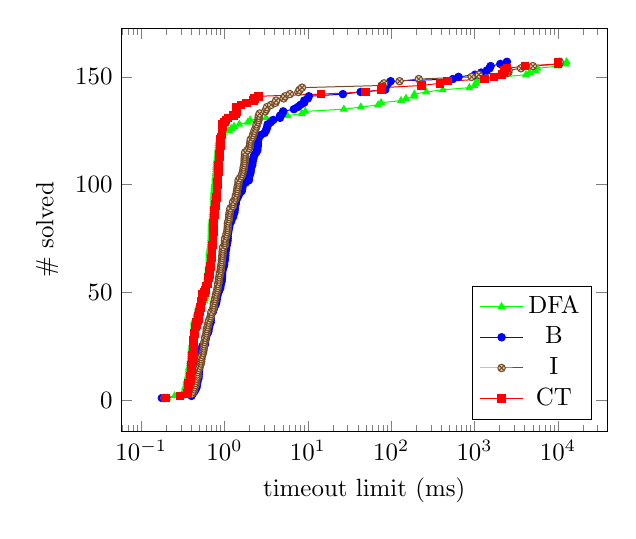
\begin{tikzpicture}[scale=0.9]
      \begin{axis}[
    xmode=log,
    every axis plot/.style={thin},
    xlabel={timeout limit (ms)},
    ylabel={\# solved},
    legend pos=south east
    % table/create on use/cumulative distribution/.style={
    %   create col/expr={\pgfmathaccuma + \thisrow{f(x)}}   
    % }
    ]
    \addplot 
    [mark=triangle*,
    mark size=1.5,
    mark options={solid},
    green] 
    coordinates {
    (0.206, 1)
(0.252, 2)
(0.327, 3)
(0.329, 4)
(0.336, 5)
(0.336, 6)
(0.347, 7)
(0.348, 8)
(0.350, 9)
(0.362, 10)
(0.363, 11)
(0.370, 12)
(0.372, 13)
(0.372, 14)
(0.373, 15)
(0.384, 16)
(0.386, 17)
(0.389, 18)
(0.391, 19)
(0.392, 20)
(0.396, 21)
(0.396, 22)
(0.397, 23)
(0.403, 24)
(0.406, 25)
(0.407, 26)
(0.416, 27)
(0.423, 28)
(0.424, 29)
(0.425, 30)
(0.428, 31)
(0.429, 32)
(0.430, 33)
(0.433, 34)
(0.434, 35)
(0.434, 36)
(0.434, 37)
(0.454, 38)
(0.459, 39)
(0.460, 40)
(0.475, 41)
(0.479, 42)
(0.483, 43)
(0.493, 44)
(0.507, 45)
(0.572, 46)
(0.580, 47)
(0.584, 48)
(0.591, 49)
(0.595, 50)
(0.596, 51)
(0.602, 52)
(0.605, 53)
(0.605, 54)
(0.607, 55)
(0.621, 56)
(0.622, 57)
(0.630, 58)
(0.635, 59)
(0.639, 60)
(0.643, 61)
(0.644, 62)
(0.650, 63)
(0.654, 64)
(0.655, 65)
(0.656, 66)
(0.657, 67)
(0.658, 68)
(0.660, 69)
(0.669, 70)
(0.672, 71)
(0.677, 72)
(0.687, 73)
(0.688, 74)
(0.689, 75)
(0.692, 76)
(0.693, 77)
(0.694, 78)
(0.695, 79)
(0.697, 80)
(0.698, 81)
(0.701, 82)
(0.705, 83)
(0.708, 84)
(0.717, 85)
(0.720, 86)
(0.723, 87)
(0.733, 88)
(0.733, 89)
(0.733, 90)
(0.737, 91)
(0.739, 92)
(0.740, 93)
(0.741, 94)
(0.743, 95)
(0.746, 96)
(0.748, 97)
(0.754, 98)
(0.757, 99)
(0.761, 100)
(0.771, 101)
(0.774, 102)
(0.774, 103)
(0.780, 104)
(0.781, 105)
(0.793, 106)
(0.794, 107)
(0.795, 108)
(0.797, 109)
(0.801, 110)
(0.805, 111)
(0.815, 112)
(0.822, 113)
(0.828, 114)
(0.832, 115)
(0.834, 116)
(0.838, 117)
(0.844, 118)
(0.846, 119)
(0.855, 120)
(0.867, 121)
(0.877, 122)
(0.949, 123)
(0.965, 124)
(1.129, 125)
(1.204, 126)
(1.301, 127)
(1.504, 128)
(1.906, 129)
(2.029, 130)
(3.141, 131)
(5.687, 132)
(8.455, 133)
(9.326, 134)
(27.018, 135)
(43.231, 136)
(69.688, 137)
(75.689, 138)
(131.214, 139)
(150.241, 140)
(189.268, 141)
(189.530, 142)
(263.729, 143)
(415.244, 144)
(867.367, 145)
(993.618, 146)
(1049.129, 147)
(1061.889, 148)
(1166.224, 149)
(2157.050, 150)
(4145.225, 151)
(4572.027, 152)
(5330.012, 153)
(5686.074, 154)
(10105.092, 155)
(12446.374, 156)
(12711.510, 157)
    };

    \addplot 
    [blue,
    mark=*,
    mark size=1.5,
    mark options={solid}]
    coordinates {
    (0.177, 1)
(0.402, 2)
(0.417, 3)
(0.434, 4)
(0.450, 5)
(0.462, 6)
(0.465, 7)
(0.469, 8)
(0.475, 9)
(0.486, 10)
(0.488, 11)
(0.490, 12)
(0.494, 13)
(0.496, 14)
(0.496, 15)
(0.498, 16)
(0.501, 17)
(0.523, 18)
(0.525, 19)
(0.527, 20)
(0.529, 21)
(0.532, 22)
(0.534, 23)
(0.542, 24)
(0.543, 25)
(0.584, 26)
(0.584, 27)
(0.590, 28)
(0.597, 29)
(0.599, 30)
(0.627, 31)
(0.641, 32)
(0.643, 33)
(0.654, 34)
(0.658, 35)
(0.681, 36)
(0.682, 37)
(0.684, 38)
(0.684, 39)
(0.694, 40)
(0.724, 41)
(0.738, 42)
(0.742, 43)
(0.774, 44)
(0.790, 45)
(0.800, 46)
(0.805, 47)
(0.814, 48)
(0.827, 49)
(0.846, 50)
(0.860, 51)
(0.888, 52)
(0.893, 53)
(0.903, 54)
(0.922, 55)
(0.926, 56)
(0.933, 57)
(0.935, 58)
(0.936, 59)
(0.945, 60)
(0.950, 61)
(0.977, 62)
(0.989, 63)
(0.990, 64)
(1.008, 65)
(1.013, 66)
(1.020, 67)
(1.023, 68)
(1.024, 69)
(1.045, 70)
(1.046, 71)
(1.062, 72)
(1.075, 73)
(1.087, 74)
(1.090, 75)
(1.090, 76)
(1.091, 77)
(1.108, 78)
(1.116, 79)
(1.135, 80)
(1.143, 81)
(1.150, 82)
(1.203, 83)
(1.212, 84)
(1.267, 85)
(1.272, 86)
(1.312, 87)
(1.318, 88)
(1.330, 89)
(1.337, 90)
(1.359, 91)
(1.369, 92)
(1.384, 93)
(1.434, 94)
(1.471, 95)
(1.518, 96)
(1.608, 97)
(1.627, 98)
(1.641, 99)
(1.652, 100)
(1.799, 101)
(1.956, 102)
(1.964, 103)
(1.976, 104)
(2.029, 105)
(2.056, 106)
(2.064, 107)
(2.079, 108)
(2.151, 109)
(2.157, 110)
(2.176, 111)
(2.215, 112)
(2.240, 113)
(2.301, 114)
(2.403, 115)
(2.475, 116)
(2.476, 117)
(2.509, 118)
(2.510, 119)
(2.512, 120)
(2.546, 121)
(2.566, 122)
(2.723, 123)
(3.025, 124)
(3.140, 125)
(3.203, 126)
(3.270, 127)
(3.296, 128)
(3.604, 129)
(3.840, 130)
(4.627, 131)
(4.636, 132)
(4.945, 133)
(5.051, 134)
(6.790, 135)
(7.543, 136)
(8.129, 137)
(9.016, 138)
(9.051, 139)
(9.998, 140)
(10.257, 141)
(26.319, 142)
(42.951, 143)
(84.403, 144)
(85.326, 145)
(86.979, 146)
(91.797, 147)
(98.458, 148)
(549.580, 149)
(641.779, 150)
(1012.231, 151)
(1201.212, 152)
(1406.365, 153)
(1513.888, 154)
(1555.971, 155)
(2037.460, 156)
(2445.578, 157)
    };

    \addplot [brown!60!black,
    mark options={fill=brown!40},
    mark=otimes*,
    mark size=1.5]
    coordinates {
    (0.189, 1)
(0.302, 2)
(0.408, 3)
(0.422, 4)
(0.433, 5)
(0.436, 6)
(0.450, 7)
(0.451, 8)
(0.458, 9)
(0.460, 10)
(0.475, 11)
(0.475, 12)
(0.476, 13)
(0.486, 14)
(0.496, 15)
(0.508, 16)
(0.519, 17)
(0.521, 18)
(0.525, 19)
(0.527, 20)
(0.541, 21)
(0.553, 22)
(0.558, 23)
(0.563, 24)
(0.566, 25)
(0.569, 26)
(0.573, 27)
(0.585, 28)
(0.585, 29)
(0.600, 30)
(0.607, 31)
(0.610, 32)
(0.612, 33)
(0.626, 34)
(0.634, 35)
(0.645, 36)
(0.652, 37)
(0.673, 38)
(0.686, 39)
(0.695, 40)
(0.697, 41)
(0.730, 42)
(0.741, 43)
(0.744, 44)
(0.745, 45)
(0.764, 46)
(0.768, 47)
(0.786, 48)
(0.788, 49)
(0.804, 50)
(0.816, 51)
(0.826, 52)
(0.834, 53)
(0.835, 54)
(0.857, 55)
(0.859, 56)
(0.864, 57)
(0.875, 58)
(0.876, 59)
(0.902, 60)
(0.902, 61)
(0.908, 62)
(0.920, 63)
(0.927, 64)
(0.928, 65)
(0.938, 66)
(0.940, 67)
(0.949, 68)
(0.949, 69)
(0.959, 70)
(0.961, 71)
(1.009, 72)
(1.010, 73)
(1.012, 74)
(1.014, 75)
(1.050, 76)
(1.054, 77)
(1.076, 78)
(1.086, 79)
(1.093, 80)
(1.095, 81)
(1.097, 82)
(1.113, 83)
(1.134, 84)
(1.139, 85)
(1.140, 86)
(1.152, 87)
(1.172, 88)
(1.178, 89)
(1.262, 90)
(1.263, 91)
(1.266, 92)
(1.329, 93)
(1.364, 94)
(1.367, 95)
(1.408, 96)
(1.409, 97)
(1.427, 98)
(1.436, 99)
(1.463, 100)
(1.473, 101)
(1.473, 102)
(1.534, 103)
(1.604, 104)
(1.636, 105)
(1.661, 106)
(1.690, 107)
(1.696, 108)
(1.721, 109)
(1.738, 110)
(1.741, 111)
(1.745, 112)
(1.753, 113)
(1.758, 114)
(1.771, 115)
(1.889, 116)
(1.979, 117)
(2.018, 118)
(2.030, 119)
(2.048, 120)
(2.065, 121)
(2.172, 122)
(2.196, 123)
(2.257, 124)
(2.289, 125)
(2.355, 126)
(2.419, 127)
(2.422, 128)
(2.520, 129)
(2.560, 130)
(2.565, 131)
(2.579, 132)
(2.642, 133)
(3.075, 134)
(3.180, 135)
(3.236, 136)
(3.623, 137)
(4.085, 138)
(4.159, 139)
(5.117, 140)
(5.335, 141)
(6.081, 142)
(7.699, 143)
(7.960, 144)
(8.507, 145)
(76.516, 146)
(82.075, 147)
(126.028, 148)
(214.042, 149)
(921.265, 150)
(1126.161, 151)
(2540.894, 152)
(2558.207, 153)
(3610.148, 154)
(5006.646, 155)
(10393.613, 156)
(10504.182, 157)
    };

    \addplot 
    [red,
    mark size=1.5,
    mark=square*]
    coordinates {
    (0.196, 1)
(0.292, 2)
(0.359, 3)
(0.362, 4)
(0.367, 5)
(0.367, 6)
(0.369, 7)
(0.370, 8)
(0.384, 9)
(0.391, 10)
(0.393, 11)
(0.396, 12)
(0.398, 13)
(0.399, 14)
(0.400, 15)
(0.403, 16)
(0.405, 17)
(0.409, 18)
(0.411, 19)
(0.411, 20)
(0.414, 21)
(0.417, 22)
(0.422, 23)
(0.423, 24)
(0.424, 25)
(0.424, 26)
(0.425, 27)
(0.427, 28)
(0.428, 29)
(0.429, 30)
(0.439, 31)
(0.440, 32)
(0.442, 33)
(0.448, 34)
(0.459, 35)
(0.461, 36)
(0.482, 37)
(0.487, 38)
(0.489, 39)
(0.494, 40)
(0.501, 41)
(0.506, 42)
(0.517, 43)
(0.519, 44)
(0.519, 45)
(0.529, 46)
(0.539, 47)
(0.543, 48)
(0.546, 49)
(0.576, 50)
(0.591, 51)
(0.597, 52)
(0.603, 53)
(0.630, 54)
(0.637, 55)
(0.638, 56)
(0.646, 57)
(0.656, 58)
(0.657, 59)
(0.661, 60)
(0.669, 61)
(0.683, 62)
(0.686, 63)
(0.690, 64)
(0.691, 65)
(0.700, 66)
(0.704, 67)
(0.704, 68)
(0.705, 69)
(0.706, 70)
(0.709, 71)
(0.720, 72)
(0.722, 73)
(0.723, 74)
(0.728, 75)
(0.729, 76)
(0.731, 77)
(0.736, 78)
(0.737, 79)
(0.738, 80)
(0.740, 81)
(0.741, 82)
(0.744, 83)
(0.752, 84)
(0.752, 85)
(0.755, 86)
(0.759, 87)
(0.761, 88)
(0.766, 89)
(0.782, 90)
(0.782, 91)
(0.787, 92)
(0.792, 93)
(0.803, 94)
(0.808, 95)
(0.811, 96)
(0.814, 97)
(0.816, 98)
(0.817, 99)
(0.826, 100)
(0.827, 101)
(0.831, 102)
(0.835, 103)
(0.836, 104)
(0.839, 105)
(0.846, 106)
(0.847, 107)
(0.850, 108)
(0.851, 109)
(0.855, 110)
(0.856, 111)
(0.859, 112)
(0.868, 113)
(0.869, 114)
(0.878, 115)
(0.880, 116)
(0.880, 117)
(0.892, 118)
(0.893, 119)
(0.898, 120)
(0.899, 121)
(0.902, 122)
(0.927, 123)
(0.933, 124)
(0.934, 125)
(0.939, 126)
(0.940, 127)
(0.940, 128)
(0.995, 129)
(1.042, 130)
(1.094, 131)
(1.287, 132)
(1.365, 133)
(1.388, 134)
(1.393, 135)
(1.396, 136)
(1.569, 137)
(1.840, 138)
(2.229, 139)
(2.291, 140)
(2.561, 141)
(14.382, 142)
(49.085, 143)
(76.751, 144)
(77.122, 145)
(231.003, 146)
(384.246, 147)
(472.162, 148)
(1311.881, 149)
(1708.022, 150)
(2131.981, 151)
(2257.100, 152)
(2279.938, 153)
(2465.965, 154)
(4014.910, 155)
(10040.100, 156)
(10092.677, 157)
    };
    \legend{DFA,B,I,CT}
  \end{axis}

    \end{tikzpicture}
    \vfill
    \caption{\textbf{Kakuro easy}.}
    \vspace{\baselineskip}
  \end{minipage}\qquad
  \end{figure}

\begin{figure}
  \begin{minipage}[b][10cm][s]{0.45\textwidth}
    \centering
    \vfill
    \begin{tikzpicture}[scale=0.9]
      \begin{axis}[
    xmode=log,
    every axis plot/.style={thin},
    xlabel={timeout limit (ms)},
    ylabel={\% solved},
    legend style={at={(0.5,-0.30)},
      anchor=north,legend columns=-1},
    % legend pos=south east,
    cycle list/Set1-6,
            % define fill color for the marker
            mark list fill={.!75!white},
            mark options={solid,scale=0.9},
            cycle multiindex* list={
                Set1-6
                    \nextlist
                [3 of]linestyles
                    \nextlist
                very thick
                \nextlist
                mark=o,
                mark=*,
                mark=square,
                mark=triangle,
                mark=+
            },
    ]

    \addplot
    coordinates {
      (1740, 7)
      (2370, 14)
      (2440, 27)
      (3030, 40)
      (3070, 47)
      (3500, 54)
      (4640, 60)
      (4670, 67)
      (4940, 74)
      (5240, 80)
      (5930, 87)
      (6460, 94)
      (7430, 100)
      
    };
    \addplot
    coordinates {
      (210, 7)
      (250, 27)
      (270, 34)
      (360, 40)
      (370, 47)
      (380, 54)
      (470, 60)
      (500, 67)
      (540, 74)
      (550, 80)
      (580, 87)
      (630, 94)
      (690, 100)
      
    };
    \addplot
    coordinates {
      (220, 7)
      (250, 14)
      (260, 27)
      (270, 34)
      (340, 40)
      (360, 47)
      (380, 54)
      (470, 60)
      (490, 67)
      (540, 80)
      (580, 87)
      (630, 94)
      (690, 100)
      
    };
    \addplot
    coordinates {
      (210, 7)
      (250, 14)
      (260, 27)
      (280, 34)
      (340, 40)
      (360, 47)
      (390, 54)
      (470, 60)
      (500, 67)
      (550, 80)
      (590, 87)
      (620, 94)
      (700, 100)
      
    };
    

    \legend{ DFA, B, I, \textbf{CT} }
  \end{axis}

    \end{tikzpicture}
    \vfill
    \caption{\textbf{Kakuro Medium}.}
    \vspace{\baselineskip}
  \end{minipage}\qquad
  \begin{minipage}[b][10cm][s]{0.45\textwidth}
    \centering
    \vfill
    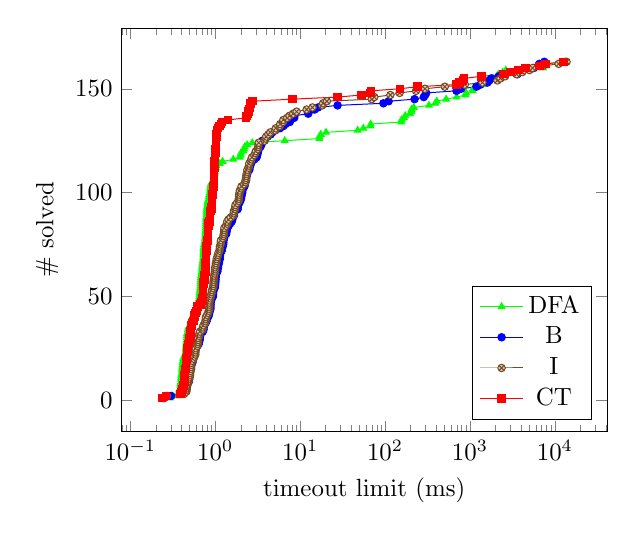
\begin{tikzpicture}[scale=0.9]
      \begin{axis}[
    xmode=log,
    every axis plot/.style={thin},
    xlabel={timeout limit (ms)},
    ylabel={\# solved},
    legend pos=south east
    % table/create on use/cumulative distribution/.style={
    %   create col/expr={\pgfmathaccuma + \thisrow{f(x)}}   
    % }
    ]
    \addplot 
    [mark=triangle*,
    mark size=1.5,
    mark options={solid},
    green] 
    coordinates {
    (0.292, 1)
(0.366, 2)
(0.373, 3)
(0.375, 4)
(0.377, 5)
(0.388, 6)
(0.389, 7)
(0.390, 8)
(0.395, 9)
(0.395, 10)
(0.397, 11)
(0.398, 12)
(0.405, 13)
(0.406, 14)
(0.406, 15)
(0.409, 16)
(0.411, 17)
(0.413, 18)
(0.416, 19)
(0.420, 20)
(0.429, 21)
(0.442, 22)
(0.446, 23)
(0.449, 24)
(0.450, 25)
(0.453, 26)
(0.454, 27)
(0.457, 28)
(0.461, 29)
(0.462, 30)
(0.462, 31)
(0.465, 32)
(0.475, 33)
(0.479, 34)
(0.483, 35)
(0.498, 36)
(0.518, 37)
(0.526, 38)
(0.532, 39)
(0.533, 40)
(0.569, 41)
(0.606, 42)
(0.615, 43)
(0.619, 44)
(0.620, 45)
(0.627, 46)
(0.628, 47)
(0.639, 48)
(0.647, 49)
(0.652, 50)
(0.655, 51)
(0.655, 52)
(0.660, 53)
(0.667, 54)
(0.670, 55)
(0.671, 56)
(0.672, 57)
(0.676, 58)
(0.678, 59)
(0.682, 60)
(0.690, 61)
(0.696, 62)
(0.697, 63)
(0.699, 64)
(0.705, 65)
(0.706, 66)
(0.714, 67)
(0.721, 68)
(0.724, 69)
(0.724, 70)
(0.725, 71)
(0.729, 72)
(0.729, 73)
(0.739, 74)
(0.740, 75)
(0.752, 76)
(0.755, 77)
(0.756, 78)
(0.762, 79)
(0.764, 80)
(0.765, 81)
(0.770, 82)
(0.773, 83)
(0.776, 84)
(0.778, 85)
(0.781, 86)
(0.782, 87)
(0.784, 88)
(0.791, 89)
(0.792, 90)
(0.792, 91)
(0.795, 92)
(0.798, 93)
(0.809, 94)
(0.811, 95)
(0.818, 96)
(0.840, 97)
(0.843, 98)
(0.850, 99)
(0.865, 100)
(0.875, 101)
(0.876, 102)
(0.879, 103)
(0.883, 104)
(0.919, 105)
(0.946, 106)
(0.956, 107)
(0.973, 108)
(0.982, 109)
(0.991, 110)
(0.993, 111)
(1.013, 112)
(1.028, 113)
(1.128, 114)
(1.220, 115)
(1.629, 116)
(1.937, 117)
(1.984, 118)
(2.002, 119)
(2.141, 120)
(2.188, 121)
(2.223, 122)
(2.373, 123)
(2.728, 124)
(6.575, 125)
(16.845, 126)
(16.868, 127)
(17.495, 128)
(20.180, 129)
(47.620, 130)
(55.482, 131)
(67.498, 132)
(67.776, 133)
(155.334, 134)
(156.640, 135)
(167.546, 136)
(172.809, 137)
(196.818, 138)
(204.653, 139)
(204.863, 140)
(217.964, 141)
(329.079, 142)
(389.985, 143)
(407.197, 144)
(523.926, 145)
(697.290, 146)
(887.001, 147)
(898.340, 148)
(1081.375, 149)
(1084.068, 150)
(1174.012, 151)
(1425.046, 152)
(1584.244, 153)
(1628.143, 154)
(1868.481, 155)
(2070.450, 156)
(2163.404, 157)
(2425.521, 158)
(2641.938, 159)
(7228.341, 160)
(7393.205, 161)
(7834.491, 162)
(13216.356, 163)
    };

    \addplot 
    [blue,
    mark=*,
    mark size=1.5,
    mark options={solid}]
    coordinates {
    (0.242, 1)
(0.303, 2)
(0.419, 3)
(0.438, 4)
(0.452, 5)
(0.458, 6)
(0.461, 7)
(0.465, 8)
(0.490, 9)
(0.493, 10)
(0.494, 11)
(0.494, 12)
(0.498, 13)
(0.503, 14)
(0.508, 15)
(0.516, 16)
(0.517, 17)
(0.538, 18)
(0.542, 19)
(0.551, 20)
(0.552, 21)
(0.565, 22)
(0.566, 23)
(0.586, 24)
(0.590, 25)
(0.612, 26)
(0.638, 27)
(0.643, 28)
(0.656, 29)
(0.657, 30)
(0.666, 31)
(0.670, 32)
(0.713, 33)
(0.729, 34)
(0.730, 35)
(0.740, 36)
(0.765, 37)
(0.789, 38)
(0.793, 39)
(0.822, 40)
(0.843, 41)
(0.848, 42)
(0.866, 43)
(0.878, 44)
(0.879, 45)
(0.881, 46)
(0.884, 47)
(0.891, 48)
(0.913, 49)
(0.941, 50)
(0.941, 51)
(0.942, 52)
(0.959, 53)
(0.984, 54)
(0.993, 55)
(0.998, 56)
(1.004, 57)
(1.007, 58)
(1.008, 59)
(1.015, 60)
(1.028, 61)
(1.060, 62)
(1.063, 63)
(1.078, 64)
(1.084, 65)
(1.105, 66)
(1.109, 67)
(1.132, 68)
(1.132, 69)
(1.139, 70)
(1.143, 71)
(1.192, 72)
(1.200, 73)
(1.223, 74)
(1.240, 75)
(1.245, 76)
(1.250, 77)
(1.268, 78)
(1.279, 79)
(1.343, 80)
(1.356, 81)
(1.369, 82)
(1.386, 83)
(1.438, 84)
(1.495, 85)
(1.561, 86)
(1.588, 87)
(1.599, 88)
(1.663, 89)
(1.671, 90)
(1.690, 91)
(1.839, 92)
(1.841, 93)
(1.864, 94)
(1.915, 95)
(1.972, 96)
(2.012, 97)
(2.023, 98)
(2.056, 99)
(2.079, 100)
(2.084, 101)
(2.117, 102)
(2.205, 103)
(2.237, 104)
(2.261, 105)
(2.308, 106)
(2.312, 107)
(2.341, 108)
(2.385, 109)
(2.398, 110)
(2.522, 111)
(2.534, 112)
(2.580, 113)
(2.639, 114)
(2.696, 115)
(2.891, 116)
(3.074, 117)
(3.110, 118)
(3.168, 119)
(3.201, 120)
(3.232, 121)
(3.395, 122)
(3.487, 123)
(3.559, 124)
(3.602, 125)
(3.912, 126)
(4.139, 127)
(4.489, 128)
(4.703, 129)
(5.104, 130)
(5.790, 131)
(6.335, 132)
(6.724, 133)
(7.557, 134)
(7.643, 135)
(8.503, 136)
(8.570, 137)
(12.437, 138)
(12.678, 139)
(14.789, 140)
(16.260, 141)
(27.598, 142)
(95.672, 143)
(110.298, 144)
(222.608, 145)
(285.892, 146)
(296.774, 147)
(305.273, 148)
(694.806, 149)
(787.648, 150)
(1192.779, 151)
(1330.528, 152)
(1607.857, 153)
(1690.387, 154)
(1785.734, 155)
(2183.007, 156)
(3619.265, 157)
(3725.830, 158)
(3776.058, 159)
(5648.925, 160)
(6436.441, 161)
(6572.117, 162)
(7516.565, 163)
    };

    \addplot [brown!60!black,
    mark options={fill=brown!40},
    mark=otimes*,
    mark size=1.5]
    coordinates {
    (0.252, 1)
(0.272, 2)
(0.430, 3)
(0.456, 4)
(0.460, 5)
(0.462, 6)
(0.469, 7)
(0.476, 8)
(0.485, 9)
(0.488, 10)
(0.499, 11)
(0.505, 12)
(0.506, 13)
(0.513, 14)
(0.520, 15)
(0.521, 16)
(0.522, 17)
(0.524, 18)
(0.536, 19)
(0.552, 20)
(0.569, 21)
(0.583, 22)
(0.583, 23)
(0.587, 24)
(0.590, 25)
(0.616, 26)
(0.620, 27)
(0.624, 28)
(0.629, 29)
(0.629, 30)
(0.648, 31)
(0.649, 32)
(0.661, 33)
(0.709, 34)
(0.715, 35)
(0.728, 36)
(0.759, 37)
(0.766, 38)
(0.774, 39)
(0.777, 40)
(0.801, 41)
(0.824, 42)
(0.842, 43)
(0.848, 44)
(0.851, 45)
(0.853, 46)
(0.854, 47)
(0.861, 48)
(0.874, 49)
(0.883, 50)
(0.899, 51)
(0.911, 52)
(0.916, 53)
(0.939, 54)
(0.952, 55)
(0.953, 56)
(0.954, 57)
(0.962, 58)
(0.966, 59)
(0.969, 60)
(0.987, 61)
(0.994, 62)
(0.999, 63)
(0.999, 64)
(1.015, 65)
(1.018, 66)
(1.036, 67)
(1.039, 68)
(1.061, 69)
(1.076, 70)
(1.094, 71)
(1.124, 72)
(1.131, 73)
(1.134, 74)
(1.160, 75)
(1.162, 76)
(1.168, 77)
(1.227, 78)
(1.249, 79)
(1.260, 80)
(1.267, 81)
(1.278, 82)
(1.282, 83)
(1.340, 84)
(1.381, 85)
(1.383, 86)
(1.432, 87)
(1.519, 88)
(1.629, 89)
(1.652, 90)
(1.656, 91)
(1.709, 92)
(1.720, 93)
(1.733, 94)
(1.812, 95)
(1.888, 96)
(1.895, 97)
(1.909, 98)
(1.912, 99)
(1.938, 100)
(1.949, 101)
(2.023, 102)
(2.043, 103)
(2.192, 104)
(2.266, 105)
(2.280, 106)
(2.309, 107)
(2.323, 108)
(2.344, 109)
(2.382, 110)
(2.391, 111)
(2.467, 112)
(2.498, 113)
(2.514, 114)
(2.612, 115)
(2.669, 116)
(2.710, 117)
(2.878, 118)
(2.960, 119)
(3.013, 120)
(3.175, 121)
(3.208, 122)
(3.231, 123)
(3.253, 124)
(3.829, 125)
(3.924, 126)
(3.993, 127)
(4.225, 128)
(4.456, 129)
(5.082, 130)
(5.168, 131)
(5.772, 132)
(5.827, 133)
(6.316, 134)
(6.346, 135)
(7.043, 136)
(7.505, 137)
(8.291, 138)
(9.089, 139)
(11.923, 140)
(13.976, 141)
(18.191, 142)
(18.643, 143)
(20.647, 144)
(69.668, 145)
(74.795, 146)
(115.506, 147)
(148.505, 148)
(231.847, 149)
(295.125, 150)
(505.755, 151)
(870.117, 152)
(1404.011, 153)
(2104.344, 154)
(2292.593, 155)
(2592.405, 156)
(3540.481, 157)
(4131.337, 158)
(5016.836, 159)
(5458.729, 160)
(7273.350, 161)
(11071.498, 162)
(13744.251, 163)
    };

    \addplot 
    [red,
    mark size=1.5,
    mark=square*]
    coordinates {
    (0.235, 1)
(0.264, 2)
(0.392, 3)
(0.398, 4)
(0.414, 5)
(0.419, 6)
(0.424, 7)
(0.431, 8)
(0.432, 9)
(0.434, 10)
(0.435, 11)
(0.437, 12)
(0.441, 13)
(0.442, 14)
(0.449, 15)
(0.450, 16)
(0.452, 17)
(0.454, 18)
(0.454, 19)
(0.457, 20)
(0.462, 21)
(0.463, 22)
(0.466, 23)
(0.472, 24)
(0.474, 25)
(0.481, 26)
(0.487, 27)
(0.493, 28)
(0.497, 29)
(0.497, 30)
(0.509, 31)
(0.509, 32)
(0.510, 33)
(0.520, 34)
(0.520, 35)
(0.528, 36)
(0.536, 37)
(0.557, 38)
(0.559, 39)
(0.570, 40)
(0.573, 41)
(0.582, 42)
(0.598, 43)
(0.608, 44)
(0.619, 45)
(0.671, 46)
(0.682, 47)
(0.707, 48)
(0.712, 49)
(0.713, 50)
(0.716, 51)
(0.716, 52)
(0.720, 53)
(0.721, 54)
(0.722, 55)
(0.725, 56)
(0.729, 57)
(0.744, 58)
(0.745, 59)
(0.749, 60)
(0.758, 61)
(0.764, 62)
(0.765, 63)
(0.767, 64)
(0.769, 65)
(0.770, 66)
(0.773, 67)
(0.775, 68)
(0.775, 69)
(0.778, 70)
(0.781, 71)
(0.785, 72)
(0.787, 73)
(0.789, 74)
(0.794, 75)
(0.803, 76)
(0.810, 77)
(0.816, 78)
(0.817, 79)
(0.819, 80)
(0.819, 81)
(0.820, 82)
(0.822, 83)
(0.832, 84)
(0.837, 85)
(0.860, 86)
(0.866, 87)
(0.867, 88)
(0.868, 89)
(0.873, 90)
(0.879, 91)
(0.901, 92)
(0.908, 93)
(0.916, 94)
(0.917, 95)
(0.919, 96)
(0.920, 97)
(0.922, 98)
(0.930, 99)
(0.942, 100)
(0.945, 101)
(0.946, 102)
(0.948, 103)
(0.960, 104)
(0.962, 105)
(0.965, 106)
(0.968, 107)
(0.969, 108)
(0.970, 109)
(0.971, 110)
(0.973, 111)
(0.974, 112)
(0.978, 113)
(0.978, 114)
(0.986, 115)
(0.990, 116)
(0.991, 117)
(0.999, 118)
(1.001, 119)
(1.007, 120)
(1.007, 121)
(1.015, 122)
(1.019, 123)
(1.021, 124)
(1.023, 125)
(1.027, 126)
(1.028, 127)
(1.030, 128)
(1.049, 129)
(1.053, 130)
(1.080, 131)
(1.119, 132)
(1.171, 133)
(1.208, 134)
(1.420, 135)
(2.298, 136)
(2.329, 137)
(2.419, 138)
(2.460, 139)
(2.514, 140)
(2.554, 141)
(2.577, 142)
(2.588, 143)
(2.747, 144)
(8.080, 145)
(27.708, 146)
(52.742, 147)
(67.644, 148)
(68.071, 149)
(149.965, 150)
(240.838, 151)
(694.991, 152)
(757.228, 153)
(832.413, 154)
(850.382, 155)
(1367.286, 156)
(2490.629, 157)
(3002.133, 158)
(3739.967, 159)
(4484.374, 160)
(6572.976, 161)
(7799.168, 162)
(12630.382, 163)
    };
    \legend{DFA,B,I,CT}
  \end{axis}

    \end{tikzpicture}
    \vfill
    \caption{\textbf{Kakuro Medium}.}
    \vspace{\baselineskip}
  \end{minipage}\qquad  
\end{figure}

\clearpage

\begin{figure}
  \begin{minipage}[b][10cm][s]{0.45\textwidth}
    \centering
    \vfill
    \begin{tikzpicture}[scale=0.9]
      \begin{axis}[
    xmode=log,
    every axis plot/.style={thin},
    xlabel={timeout limit (ms)},
    ylabel={\% solved},
    legend style={at={(0.5,-0.30)},
      anchor=north,legend columns=-1},
    % legend pos=south east,
    cycle list/Set1-6,
            % define fill color for the marker
            mark list fill={.!75!white},
            mark options={solid,scale=0.9},
            cycle multiindex* list={
                Set1-6
                    \nextlist
                [3 of]linestyles
                    \nextlist
                very thick
                \nextlist
                mark=o,
                mark=*,
                mark=square,
                mark=triangle,
                mark=+
            },
    ]

    \addplot
    coordinates {
      (1030, 8)
      (2420, 16)
      (2630, 24)
      (2760, 31)
      (2910, 39)
      (3260, 47)
      (3700, 54)
      (4820, 62)
      (5260, 70)
      (5970, 77)
      (6170, 85)
      (6400, 93)
      (6620, 100)
      
    };
    \addplot
    coordinates {
      (170, 8)
      (240, 16)
      (260, 24)
      (290, 31)
      (300, 39)
      (320, 47)
      (350, 54)
      (420, 62)
      (440, 70)
      (500, 77)
      (520, 85)
      (560, 93)
      (590, 100)
      
    };
    \addplot
    coordinates {
      (180, 8)
      (240, 16)
      (260, 24)
      (280, 31)
      (300, 39)
      (320, 47)
      (350, 54)
      (420, 62)
      (440, 70)
      (500, 77)
      (520, 85)
      (570, 93)
      (600, 100)
      
    };
    \addplot
    coordinates {
      (170, 8)
      (240, 16)
      (260, 24)
      (280, 31)
      (300, 39)
      (320, 47)
      (350, 54)
      (420, 62)
      (440, 70)
      (490, 77)
      (520, 85)
      (570, 93)
      (610, 100)
      
    };
    

    \legend{ DFA, B, I, \textbf{CT} }
  \end{axis}

    \end{tikzpicture}
    \vfill
    \caption{\textbf{Kakuro Hard}.}
    \vspace{\baselineskip}
  \end{minipage}\qquad
  \begin{minipage}[b][10cm][s]{0.45\textwidth}
    \centering
    \vfill
    \begin{tikzpicture}[scale=0.9]
      \begin{axis}[
    xmode=log,
    every axis plot/.style={thin},
    xlabel={timeout limit (ms)},
    ylabel={\% solved},
    legend pos=south east,
    cycle list/Set1-6,
            % define fill color for the marker
            mark list fill={.!75!white},
            mark options={solid},
            cycle multiindex* list={
                Set1-6
                    \nextlist
                [3 of]linestyles
                    \nextlist
                very thick
                \nextlist
                mark=o,
                mark=*,
                mark=square,
                mark=triangle,
                mark=+
            },
    ]

    

    \legend{ DFA, B, I, \textbf{CT} }
  \end{axis}

    \end{tikzpicture}
    \vfill
    \caption{\textbf{Kakuro Hard}.}
    \vspace{\baselineskip}
  \end{minipage}\qquad

\end{figure}

\begin{figure}
  \begin{minipage}[b][10cm][s]{0.45\textwidth}
    \centering
    \vfill
    \begin{tikzpicture}[scale=0.9]
      \begin{axis}[
    xmode=log,
    every axis plot/.style={thin},
    xlabel={timeout limit (ms)},
    ylabel={\% solved},
    legend pos=south east,
    cycle list/Set1-6,
            % define fill color for the marker
            mark list fill={.!75!white},
            mark options={solid},
            cycle multiindex* list={
                Set1-6
                    \nextlist
                [3 of]linestyles
                    \nextlist
                very thick
                \nextlist
                mark=o,
                mark=*,
                mark=square,
                mark=triangle,
                mark=+
            },
    ]

    \addplot
    coordinates {
      (2310, 7)
      (3050, 14)
      (3280, 20)
      (3480, 27)
      (4110, 34)
      (4640, 40)
      (6230, 47)
      (6550, 54)
      (6570, 60)
      (7330, 67)
      (7780, 74)
      (8210, 80)
      (8270, 87)
      (8360, 94)
      (12510, 100)
      
    };
    \addplot
    coordinates {
      (610, 7)
      (820, 14)
      (990, 20)
      (1200, 27)
      (1250, 34)
      (1530, 40)
      (8430, 47)
      (8550, 54)
      (13190, 60)
      (14750, 67)
      (22720, 74)
      (26230, 80)
      (34060, 87)
      (99550, 94)
      (196100, 100)
      
    };
    \addplot
    coordinates {
      (720, 7)
      (1040, 14)
      (1180, 20)
      (1570, 27)
      (1610, 34)
      (2060, 40)
      (11310, 47)
      (12140, 54)
      (17130, 60)
      (19510, 67)
      (31680, 74)
      (37680, 80)
      (47500, 87)
      (136970, 94)
      (261960, 100)
      
    };
    \addplot
    coordinates {
      (400, 7)
      (550, 14)
      (560, 20)
      (630, 27)
      (690, 34)
      (800, 40)
      (3710, 47)
      (3760, 54)
      (5650, 60)
      (5810, 67)
      (9780, 74)
      (10930, 80)
      (13290, 87)
      (43980, 94)
      (77540, 100)
      
    };
    

    \legend{ DFA, B, I, \textbf{CT} }
  \end{axis}

    \end{tikzpicture}
    \vfill
    \caption{\textbf{TSP 25}.}
    \vspace{\baselineskip}
  \end{minipage}\qquad
  \begin{minipage}[b][10cm][s]{0.45\textwidth}
    \centering
    \vfill
    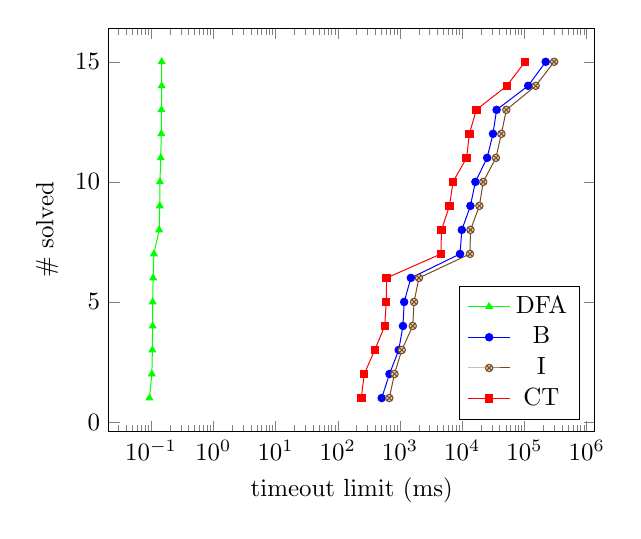
\begin{tikzpicture}[scale=0.9]
      \begin{axis}[
    xmode=log,
    every axis plot/.style={thin},
    xlabel={timeout limit (ms)},
    ylabel={\# solved},
    legend pos=south east
    % table/create on use/cumulative distribution/.style={
    %   create col/expr={\pgfmathaccuma + \thisrow{f(x)}}   
    % }
    ]
    \addplot 
    [mark=triangle*,
    mark size=1.5,
    mark options={solid},
    green] 
    coordinates {
    (0.094, 1)
(0.103, 2)
(0.105, 3)
(0.106, 4)
(0.106, 5)
(0.108, 6)
(0.111, 7)
(0.135, 8)
(0.138, 9)
(0.139, 10)
(0.143, 11)
(0.146, 12)
(0.147, 13)
(0.148, 14)
(0.148, 15)
    };

    \addplot 
    [blue,
    mark=*,
    mark size=1.5,
    mark options={solid}]
    coordinates {
    (507.741, 1)
(677.384, 2)
(953.532, 3)
(1115.834, 4)
(1165.768, 5)
(1493.977, 6)
(9207.006, 7)
(9850.063, 8)
(13526.871, 9)
(16256.105, 10)
(25103.486, 11)
(31196.630, 12)
(35646.183, 13)
(114674.413, 14)
(219336.179, 15)
    };

    \addplot [brown!60!black,
    mark options={fill=brown!40},
    mark=otimes*,
    mark size=1.5]
    coordinates {
    (672.485, 1)
(814.969, 2)
(1067.305, 3)
(1600.629, 4)
(1680.609, 5)
(2014.622, 6)
(13301.506, 7)
(13571.938, 8)
(18857.094, 9)
(21725.057, 10)
(34735.363, 11)
(42587.462, 12)
(51076.269, 13)
(151568.002, 14)
(299369.282, 15)
    };

    \addplot 
    [red,
    mark size=1.5,
    mark=square*]
    coordinates {
    (238.429, 1)
(266.356, 2)
(392.689, 3)
(568.593, 4)
(600.935, 5)
(609.600, 6)
(4557.050, 7)
(4627.268, 8)
(6237.444, 9)
(7103.168, 10)
(11748.022, 11)
(13000.044, 12)
(16831.605, 13)
(52006.921, 14)
(102348.407, 15)
    };
    \legend{DFA,B,I,CT}
  \end{axis}

    \end{tikzpicture}
    \vfill
    \caption{\textbf{TSP 25}.}
    \vspace{\baselineskip}
  \end{minipage}\qquad
\end{figure}
\begin{figure}
  \begin{minipage}[b][10cm][s]{0.45\textwidth}
    \centering
    \vfill
    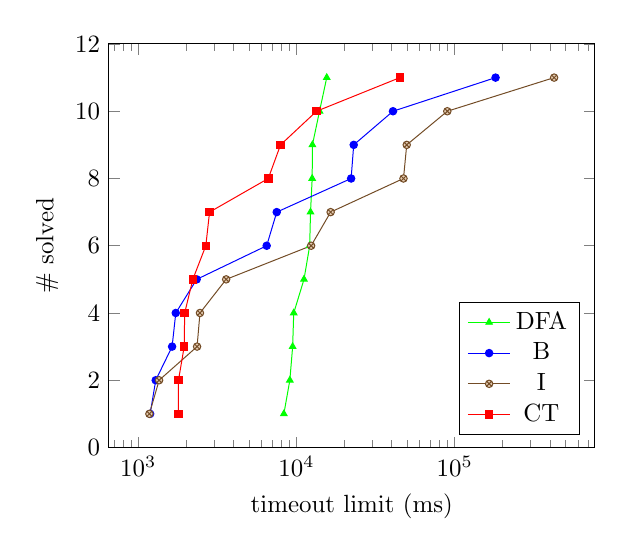
\begin{tikzpicture}[scale=0.9]
      \begin{axis}[
    xmode=log,
    every axis plot/.style={thin},
    xlabel={timeout limit (ms)},
    ylabel={\# solved},
    legend pos=south east
    % table/create on use/cumulative distribution/.style={
    %   create col/expr={\pgfmathaccuma + \thisrow{f(x)}}   
    % }
    ]
    \addplot 
    [mark=triangle*,
    mark size=1.5,
    mark options={solid},
    green] 
    coordinates {
    (8323.942, 1)
(9080.418, 2)
(9457.327, 3)
(9611.154, 4)
(11157.909, 5)
(12122.318, 6)
(12269.578, 7)
(12569.631, 8)
(12613.425, 9)
(13987.860, 10)
(15538.867, 11)
    };

    \addplot 
    [blue,
    mark=*,
    mark size=1.5,
    mark options={solid}]
    coordinates {
    (1188.206, 1)
(1289.021, 2)
(1636.318, 3)
(1725.962, 4)
(2339.887, 5)
(6481.991, 6)
(7504.933, 7)
(22155.924, 8)
(23009.793, 9)
(40756.444, 10)
(181399.438, 11)
    };

    \addplot [brown!60!black,
    mark options={fill=brown!40},
    mark=otimes*,
    mark size=1.5]
    coordinates {
    (1175.718, 1)
(1354.438, 2)
(2353.159, 3)
(2454.453, 4)
(3594.396, 5)
(12379.752, 6)
(16444.353, 7)
(47478.184, 8)
(49773.525, 9)
(89852.322, 10)
(425399.368, 11)
    };

    \addplot 
    [red,
    mark size=1.5,
    mark=square*]
    coordinates {
    (1794.640, 1)
(1795.355, 2)
(1951.150, 3)
(1965.074, 4)
(2212.001, 5)
(2673.018, 6)
(2822.171, 7)
(6633.134, 8)
(7933.220, 9)
(13389.469, 10)
(45079.672, 11)
    };
    \legend{DFA,B,I,CT}
  \end{axis}

    \end{tikzpicture}
    \vfill
    \caption{\textbf{TSP Quat 20}.}
    \vspace{\baselineskip}
  \end{minipage}\qquad
    \begin{minipage}[b][10cm][s]{0.45\textwidth}
    \centering
    \vfill
    \begin{tikzpicture}[scale=0.9]
      \begin{axis}[
    xmode=log,
    every axis plot/.style={thin},
    xlabel={timeout limit (ms)},
    ylabel={\% solved},
    legend pos=south east,
    cycle list/Set1-6,
            % define fill color for the marker
            mark list fill={.!75!white},
            mark options={solid},
            cycle multiindex* list={
                Set1-6
                    \nextlist
                [3 of]linestyles
                    \nextlist
                very thick
                \nextlist
                mark=o,
                mark=*,
                mark=square,
                mark=triangle,
                mark=+
            },
    ]

    \addplot
    coordinates {
      (10, 100)
      
    };
    \addplot
    coordinates {
      (450, 9)
      (1090, 17)
      (4880, 25)
      (6570, 34)
      (10500, 42)
      (20600, 50)
      (20960, 59)
      (22090, 67)
      (38950, 75)
      (42650, 84)
      (75800, 92)
      (188330, 100)
      
    };
    \addplot
    coordinates {
      (1070, 9)
      (2170, 17)
      (10820, 25)
      (15550, 34)
      (22220, 42)
      (44210, 50)
      (45960, 59)
      (48540, 67)
      (90190, 75)
      (98750, 84)
      (158640, 92)
      (433210, 100)
      
    };
    \addplot
    coordinates {
      (80, 9)
      (180, 17)
      (550, 25)
      (660, 34)
      (1640, 42)
      (3210, 50)
      (3620, 59)
      (4490, 67)
      (6250, 75)
      (8070, 84)
      (11340, 92)
      (32170, 100)
      
    };
    

    \legend{ DFA, B, I, \textbf{CT} }
  \end{axis}

    \end{tikzpicture}
    \vfill
    \caption{\textbf{TSP Quat 20}.}
    \vspace{\baselineskip}
  \end{minipage}\qquad
\end{figure}

\clearpage

\begin{figure}
  \begin{minipage}[b][10cm][s]{0.45\textwidth}
    \centering
    \vfill
    \begin{tikzpicture}[scale=0.9]
      %\begin{axis}[
    xmode=log,
    every axis plot/.style={thin},
    xlabel={timeout limit (ms)},
    ylabel={\# solved},
    legend pos=north east
    % table/create on use/cumulative distribution/.style={
    %   create col/expr={\pgfmathaccuma + \thisrow{f(x)}}   
    % }
    ]
    \addplot 
    [mark=triangle*,
    mark size=1.5,
    mark options={solid},
    green] 
    coordinates {
    (14955.640, 1)
(14968.715, 2)
(15081.852, 3)
(15246.230, 4)
(15319.517, 5)
(15694.443, 6)
(15719.960, 7)
(15775.606, 8)
(15786.850, 9)
(15896.231, 10)
(15965.343, 11)
(16005.555, 12)
(16025.117, 13)
(16031.876, 14)
(16045.846, 15)
(16051.370, 16)
(16069.886, 17)
(16072.811, 18)
(16083.237, 19)
(16121.665, 20)
(16136.113, 21)
(16156.801, 22)
(16176.375, 23)
(16178.653, 24)
(16245.676, 25)
(16366.799, 26)
(16378.158, 27)
(16380.892, 28)
(16416.757, 29)
(16478.895, 30)
(16497.038, 31)
(16500.046, 32)
(16533.794, 33)
(16540.436, 34)
(16585.806, 35)
(16652.982, 36)
(16691.128, 37)
(16800.390, 38)
(16810.154, 39)
(16925.261, 40)
(16928.061, 41)
(17203.760, 42)
(17283.698, 43)
(17423.272, 44)
(17512.601, 45)
(17538.616, 46)
(17769.707, 47)
(18045.623, 48)
(18343.375, 49)
    };

    \addplot 
    [blue,
    mark=*,
    mark size=1.5,
    mark options={solid}]
    coordinates {
    (407.759, 1)
(414.434, 2)
(419.216, 3)
(450.778, 4)
(549.394, 5)
(610.163, 6)
(686.273, 7)
(1398.874, 8)
(15928.727, 9)
(49039.533, 10)
(59721.595, 11)
(169215.924, 12)
(415997.085, 13)
(649968.448, 14)
(907521.385, 15)
% (1000382.106, 16)
% (1000387.429, 17)
% (1000388.151, 18)
% (1000388.347, 19)
% (1000390.684, 20)
% (1000395.468, 21)
% (1000398.451, 22)
% (1000400.524, 23)
% (1000400.706, 24)
% (1000401.730, 25)
% (1000401.841, 26)
% (1000403.654, 27)
% (1000403.994, 28)
% (1000404.160, 29)
% (1000404.725, 30)
% (1000405.072, 31)
% (1000406.271, 32)
% (1000406.289, 33)
% (1000408.137, 34)
% (1000409.168, 35)
% (1000409.171, 36)
% (1000409.900, 37)
% (1000409.919, 38)
% (1000410.346, 39)
% (1000411.211, 40)
% (1000412.274, 41)
% (1000412.434, 42)
% (1000413.669, 43)
% (1000413.697, 44)
% (1000413.893, 45)
% (1000415.159, 46)
% (1000415.655, 47)
% (1000416.766, 48)
% (1000417.147, 49)
    };

    \addplot [brown!60!black,
    mark options={fill=brown!40},
    mark=otimes*,
    mark size=1.5]
    coordinates {
    (411.425, 1)
(411.643, 2)
(429.292, 3)
(468.693, 4)
(639.628, 5)
(667.122, 6)
(794.022, 7)
(2406.553, 8)
(23078.974, 9)
(62957.355, 10)
(104153.981, 11)
(249841.503, 12)
(558201.118, 13)
% (1000388.044, 14)
% (1000402.477, 15)
% (1000403.436, 16)
% (1000404.783, 17)
% (1000405.378, 18)
% (1000405.704, 19)
% (1000406.897, 20)
% (1000406.968, 21)
% (1000407.434, 22)
% (1000407.466, 23)
% (1000408.430, 24)
% (1000410.331, 25)
% (1000411.890, 26)
% (1000412.483, 27)
% (1000413.619, 28)
% (1000413.815, 29)
% (1000414.349, 30)
% (1000417.491, 31)
% (1000417.949, 32)
% (1000418.050, 33)
% (1000418.110, 34)
% (1000419.106, 35)
% (1000421.213, 36)
% (1000425.194, 37)
% (1000425.968, 38)
% (1000429.409, 39)
% (1000430.069, 40)
% (1000430.274, 41)
% (1000431.550, 42)
% (1000431.958, 43)
% (1000434.278, 44)
% (1000435.376, 45)
% (1000437.954, 46)
% (1000465.864, 47)
% (1000470.438, 48)
% (1000485.931, 49)
    };

    \addplot 
    [red,
    mark size=1.5,
    mark=square*]
    coordinates {
    (508.071, 1)
(509.196, 2)
(510.855, 3)
(534.756, 4)
(578.458, 5)
(581.294, 6)
(592.155, 7)
(871.362, 8)
(6376.939, 9)
(14282.674, 10)
(18970.185, 11)
(61800.545, 12)
(171097.990, 13)
(328543.590, 14)
(399691.539, 15)
% (1000508.452, 16)
% (1000510.576, 17)
% (1000511.037, 18)
% (1000515.800, 19)
% (1000516.296, 20)
% (1000522.133, 21)
% (1000522.266, 22)
% (1000527.510, 23)
% (1000527.510, 24)
% (1000530.273, 25)
% (1000530.582, 26)
% (1000535.684, 27)
% (1000536.663, 28)
% (1000538.258, 29)
% (1000538.752, 30)
% (1000538.821, 31)
% (1000539.927, 32)
% (1000542.929, 33)
% (1000543.075, 34)
% (1000543.682, 35)
% (1000543.865, 36)
% (1000547.730, 37)
% (1000548.803, 38)
% (1000549.065, 39)
% (1000549.762, 40)
% (1000552.156, 41)
% (1000552.610, 42)
% (1000560.835, 43)
% (1000562.921, 44)
% (1000565.715, 45)
% (1000567.437, 46)
% (1000570.129, 47)
% (1000576.494, 48)
% (1000627.930, 49)
    };
    \legend{DFA,B,I,CT}
  \end{axis}

    \end{tikzpicture}
    \vfill
    \caption{\textbf{Mod Renault}.}
    \vspace{\baselineskip}
  \end{minipage}\qquad
  \begin{minipage}[b][10cm][s]{0.45\textwidth}
    \centering
    \vfill
    \begin{tikzpicture}[scale=0.9]
      %\begin{axis}[
    xmode=log,
    every axis plot/.style={thin},
    xlabel={timeout limit (ms)},
    ylabel={\# solved},
    legend pos=north east
    % table/create on use/cumulative distribution/.style={
    %   create col/expr={\pgfmathaccuma + \thisrow{f(x)}}   
    % }
    ]
    \addplot 
    [mark=triangle*,
    mark size=1.5,
    mark options={solid},
    green] 
    coordinates {
    (0.090, 1)
(0.092, 2)
(0.094, 3)
(0.094, 4)
(0.094, 5)
(0.095, 6)
(0.095, 7)
(0.095, 8)
(0.096, 9)
(0.096, 10)
(0.096, 11)
(0.097, 12)
(0.098, 13)
(0.098, 14)
(0.098, 15)
(0.098, 16)
(0.098, 17)
(0.099, 18)
(0.099, 19)
(0.099, 20)
(0.099, 21)
(0.099, 22)
(0.099, 23)
(0.099, 24)
(0.099, 25)
(0.100, 26)
(0.101, 27)
(0.102, 28)
(0.125, 29)
(0.127, 30)
(0.127, 31)
(0.128, 32)
(0.129, 33)
(0.130, 34)
(0.130, 35)
(0.130, 36)
(0.131, 37)
(0.133, 38)
(0.133, 39)
(0.133, 40)
(0.134, 41)
(0.136, 42)
(0.137, 43)
(0.137, 44)
(0.139, 45)
(0.141, 46)
(0.142, 47)
(0.147, 48)
(0.150, 49)
    };

    \addplot 
    [blue,
    mark=*,
    mark size=1.5,
    mark options={solid}]
    coordinates {
    (8.908, 1)
(9.827, 2)
(18.048, 3)
(44.969, 4)
(146.544, 5)
(221.926, 6)
(280.600, 7)
(1000.181, 8)
(15513.013, 9)
(48631.945, 10)
(59316.805, 11)
(168805.480, 12)
(415608.611, 13)
(649574.201, 14)
(907115.910, 15)
% (1000000.555, 16)
% (1000000.559, 17)
% (1000000.602, 18)
% (1000000.610, 19)
% (1000000.620, 20)
% (1000000.629, 21)
% (1000000.647, 22)
% (1000000.658, 23)
% (1000000.659, 24)
% (1000000.668, 25)
% (1000000.676, 26)
% (1000000.690, 27)
% (1000000.697, 28)
% (1000000.698, 29)
% (1000000.703, 30)
% (1000000.711, 31)
% (1000000.711, 32)
% (1000000.726, 33)
% (1000000.733, 34)
% (1000000.760, 35)
% (1000000.775, 36)
% (1000000.777, 37)
% (1000000.783, 38)
% (1000000.783, 39)
% (1000000.818, 40)
% (1000000.834, 41)
% (1000000.837, 42)
% (1000000.841, 43)
% (1000000.891, 44)
% (1000000.911, 45)
% (1000001.014, 46)
% (1000001.027, 47)
% (1000001.082, 48)
% (1000001.151, 49)
    };

    \addplot [brown!60!black,
    mark options={fill=brown!40},
    mark=otimes*,
    mark size=1.5]
    coordinates {
    (8.888, 1)
(10.058, 2)
(23.562, 3)
(63.830, 4)
(252.102, 5)
(271.618, 6)
(388.958, 7)
(2008.685, 8)
(22663.365, 9)
(62548.705, 10)
(103749.263, 11)
(249342.517, 12)
(557770.707, 13)
% (1000000.164, 14)
% (1000000.168, 15)
% (1000000.168, 16)
% (1000000.170, 17)
% (1000000.177, 18)
% (1000000.180, 19)
% (1000000.188, 20)
% (1000000.189, 21)
% (1000000.189, 22)
% (1000000.201, 23)
% (1000000.207, 24)
% (1000000.210, 25)
% (1000000.227, 26)
% (1000000.239, 27)
% (1000000.243, 28)
% (1000000.243, 29)
% (1000000.248, 30)
% (1000000.252, 31)
% (1000000.253, 32)
% (1000000.253, 33)
% (1000000.270, 34)
% (1000000.294, 35)
% (1000000.295, 36)
% (1000000.300, 37)
% (1000000.313, 38)
% (1000000.316, 39)
% (1000000.323, 40)
% (1000000.347, 41)
% (1000000.375, 42)
% (1000000.438, 43)
% (1000000.448, 44)
% (1000000.542, 45)
% (1000000.561, 46)
% (1000000.574, 47)
% (1000000.653, 48)
% (1000001.050, 49)
    };

    \addplot 
    [red,
    mark size=1.5,
    mark=square*]
    coordinates {
    (2.210, 1)
(2.770, 2)
(5.373, 3)
(14.096, 4)
(50.117, 5)
(54.652, 6)
(63.872, 7)
(349.605, 8)
(5835.733, 9)
(13759.320, 10)
(18438.411, 11)
(61277.615, 12)
(170563.334, 13)
(328014.772, 14)
(399164.764, 15)
% (1000000.135, 16)
% (1000000.135, 17)
% (1000000.145, 18)
% (1000000.147, 19)
% (1000000.151, 20)
% (1000000.152, 21)
% (1000000.154, 22)
% (1000000.156, 23)
% (1000000.156, 24)
% (1000000.160, 25)
% (1000000.164, 26)
% (1000000.168, 27)
% (1000000.178, 28)
% (1000000.206, 29)
% (1000000.211, 30)
% (1000000.214, 31)
% (1000000.217, 32)
% (1000000.222, 33)
% (1000000.223, 34)
% (1000000.226, 35)
% (1000000.232, 36)
% (1000000.233, 37)
% (1000000.243, 38)
% (1000000.246, 39)
% (1000000.253, 40)
% (1000000.290, 41)
% (1000000.300, 42)
% (1000000.320, 43)
% (1000000.326, 44)
% (1000000.412, 45)
% (1000000.588, 46)
% (1000000.601, 47)
% (1000000.734, 48)
% (1000000.739, 49)
    };
    \legend{DFA,B,I,CT}
  \end{axis}

    \end{tikzpicture}
    \vfill
    \caption{\textbf{Mod Renault}.}
    \vspace{\baselineskip}
  \end{minipage}\qquad
\end{figure}
\begin{figure}

  \begin{minipage}[b][10cm][s]{0.45\textwidth}
    \centering
    \vfill
    \begin{tikzpicture}[scale=0.9]
      \begin{axis}[
    xmode=log,
    every axis plot/.style={thin},
    xlabel={timeout limit (ms)},
    ylabel={\% solved},
    legend style={at={(0.5,-0.30)},
      anchor=north,legend columns=-1},
    % legend pos=south east,
    cycle list/Set1-6,
            % define fill color for the marker
            mark list fill={.!75!white},
            mark options={solid,scale=0.9},
            cycle multiindex* list={
                Set1-6
                    \nextlist
                [3 of]linestyles
                    \nextlist
                very thick
                \nextlist
                mark=o,
                mark=*,
                mark=square,
                mark=triangle,
                mark=+
            },
    ]

    \addplot
    coordinates {
      (550, 7)
      (1420, 13)
      (2180, 19)
      (2460, 25)
      (4050, 32)
      (11860, 38)
      (37590, 44)
      (42030, 50)
      (51040, 57)
      (744510, 63)
      (828510, 69)
      (921350, 75)
      
    };
    \addplot
    coordinates {
      (730, 7)
      (2790, 13)
      (2950, 19)
      (9950, 25)
      (22390, 32)
      (55820, 38)
      (79890, 44)
      (247070, 50)
      
    };
    \addplot
    coordinates {
      (720, 7)
      (2880, 13)
      (4460, 19)
      (11570, 25)
      (21880, 32)
      (80590, 38)
      (84470, 44)
      (276470, 50)
      
    };
    \addplot
    coordinates {
      (140, 7)
      (210, 13)
      (680, 19)
      (1410, 25)
      (1760, 32)
      (2610, 38)
      (23590, 44)
      (29830, 50)
      (49050, 57)
      (474090, 63)
      (606460, 69)
      
    };
    

    \legend{ DFA, B, I, \textbf{CT} }
  \end{axis}

    \end{tikzpicture}
    \vfill
    \caption{\textbf{Pigeons Plus}.}
    \vspace{\baselineskip}
  \end{minipage}\qquad
  \begin{minipage}[b][10cm][s]{0.45\textwidth}
    \centering
    \vfill
    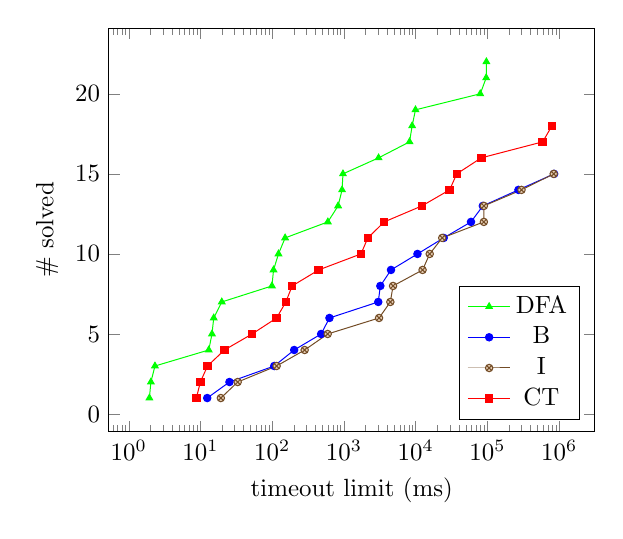
\begin{tikzpicture}[scale=0.9]
      \begin{axis}[
    xmode=log,
    every axis plot/.style={thin},
    xlabel={timeout limit (ms)},
    ylabel={\# solved},
    legend pos=south east
    % table/create on use/cumulative distribution/.style={
    %   create col/expr={\pgfmathaccuma + \thisrow{f(x)}}   
    % }
    ]
    \addplot 
    [mark=triangle*,
    mark size=1.5,
    mark options={solid},
    green] 
    coordinates {
    (1.939, 1)
(2.035, 2)
(2.317, 3)
(13.027, 4)
(14.455, 5)
(15.287, 6)
(19.798, 7)
(99.029, 8)
(104.241, 9)
(122.179, 10)
(151.134, 11)
(595.639, 12)
(828.083, 13)
(940.207, 14)
(967.914, 15)
(3036.095, 16)
(8198.788, 17)
(8913.808, 18)
(9922.558, 19)
(79329.149, 20)
(96050.608, 21)
(96605.875, 22)
%(106404.530, 23)
    };

    \addplot 
    [blue,
    mark=*,
    mark size=1.5,
    mark options={solid}]
    coordinates {
    (12.405, 1)
(25.327, 2)
(106.527, 3)
(202.145, 4)
(480.401, 5)
(627.315, 6)
(3003.911, 7)
(3211.723, 8)
(4522.000, 9)
(10582.965, 10)
(24531.228, 11)
(58955.686, 12)
(86209.530, 13)
(270270.395, 14)
(849755.006, 15)
% (1000000.185, 16)
% (1000000.224, 17)
% (1000000.242, 18)
% (1000000.270, 19)
% (1000000.315, 20)
% (1000000.495, 21)
% (1000000.854, 22)
% (1000003.143, 23)
    };

    \addplot [brown!60!black,
    mark options={fill=brown!40},
    mark=otimes*,
    mark size=1.5]
    coordinates {
    (19.206, 1)
(32.979, 2)
(115.009, 3)
(283.034, 4)
(592.721, 5)
(3080.707, 6)
(4428.906, 7)
(4826.985, 8)
(12458.187, 9)
(15667.538, 10)
(23411.812, 11)
(89065.097, 12)
(89238.217, 13)
(298360.864, 14)
(837935.273, 15)
% (1000000.180, 16)
% (1000000.230, 17)
% (1000000.490, 18)
% (1000002.486, 19)
% (1000004.375, 20)
% (1000005.069, 21)
% (1024308.427, 22)
% (1028402.839, 23)
    };

    \addplot 
    [red,
    mark size=1.5,
    mark=square*]
    coordinates {
    (8.749, 1)
(9.961, 2)
(12.509, 3)
(21.552, 4)
(52.342, 5)
(115.051, 6)
(154.775, 7)
(189.472, 8)
(443.467, 9)
(1726.716, 10)
(2147.900, 11)
(3639.810, 12)
(12209.023, 13)
(29682.808, 14)
(37338.185, 15)
(81990.479, 16)
(588724.922, 17)
(792421.490, 18)
% (1002937.685, 19)
% (1006307.166, 20)
% (1040367.757, 21)
% (1043510.024, 22)
% (1054819.699, 23)
    };
    \legend{DFA,B,I,CT}
  \end{axis}

    \end{tikzpicture}
    \vfill
    \caption{\textbf{Pigeons Plus}.}
    \vspace{\baselineskip}
  \end{minipage}\qquad

\end{figure}

\clearpage

\begin{figure}

  \begin{minipage}[b][10cm][s]{0.45\textwidth}
    \centering
    \vfill
    \begin{tikzpicture}[scale=0.9]
      \begin{axis}[
    xmode=log,
    every axis plot/.style={thin},
    xlabel={timeout limit (ms)},
    ylabel={\# solved},
    legend pos=south east
    % table/create on use/cumulative distribution/.style={
    %   create col/expr={\pgfmathaccuma + \thisrow{f(x)}}   
    % }
    ]
    \addplot 
    [mark=triangle*,
    mark size=1.5,
    mark options={solid},
    green] 
    coordinates {
    (7669.883, 1)
(8836.338, 2)
(8977.330, 3)
(9140.777, 4)
(11537.562, 5)
(13231.384, 6)
(14923.762, 7)
(15381.136, 8)
(15623.402, 9)
(16994.255, 10)
    };

    \addplot 
    [blue,
    mark=*,
    mark size=1.5,
    mark options={solid}]
    coordinates {
    (8538.228, 1)
(12749.685, 2)
(18156.956, 3)
(18327.323, 4)
(19669.292, 5)
(28802.590, 6)
(30835.715, 7)
(40301.654, 8)
(48620.995, 9)
(50774.009, 10)
    };

    \addplot [brown!60!black,
    mark options={fill=brown!40},
    mark=otimes*,
    mark size=1.5]
    coordinates {
    (9960.047, 1)
(13326.927, 2)
(20700.530, 3)
(21474.840, 4)
(21842.271, 5)
(33817.893, 6)
(35489.987, 7)
(48049.593, 8)
(53196.297, 9)
(55499.785, 10)
    };

    \addplot 
    [red,
    mark size=1.5,
    mark=square*]
    coordinates {
    (1591.239, 1)
(1678.457, 2)
(2251.773, 3)
(2462.919, 4)
(2646.514, 5)
(3745.993, 6)
(4020.526, 7)
(4095.836, 8)
(5320.617, 9)
(5507.353, 10)
    };
    \legend{DFA,B,I,\textbf{CT}}
  \end{axis}

    \end{tikzpicture}
    \vfill
    \caption{\textbf{K5}.}
    \vspace{\baselineskip}
  \end{minipage}\qquad
  \begin{minipage}[b][10cm][s]{0.45\textwidth}
    \centering
    \vfill
    \begin{tikzpicture}[scale=0.9]
      \begin{axis}[
    xmode=log,
    every axis plot/.style={thin},
    xlabel={timeout limit (ms)},
    ylabel={\% solved},
    legend pos=south east,
    cycle list/Set1-6,
            % define fill color for the marker
            mark list fill={.!75!white},
            mark options={solid},
            cycle multiindex* list={
                Set1-6
                    \nextlist
                [3 of]linestyles
                    \nextlist
                very thick
                \nextlist
                mark=o,
                mark=*,
                mark=square,
                mark=triangle,
                mark=+
            },
    ]

    \addplot
    coordinates {
      (4940, 10)
      (5170, 20)
      (5550, 30)
      (5870, 40)
      (8370, 50)
      (11130, 60)
      (12340, 70)
      (12510, 80)
      (13080, 90)
      (14360, 100)
      
    };
    \addplot
    coordinates {
      (8230, 10)
      (12520, 20)
      (16360, 30)
      (16890, 40)
      (19380, 50)
      (27950, 60)
      (30990, 70)
      (40600, 80)
      (46310, 90)
      (48240, 100)
      
    };
    \addplot
    coordinates {
      (9330, 10)
      (12070, 20)
      (18830, 30)
      (19890, 40)
      (20740, 50)
      (33400, 60)
      (34230, 70)
      (47110, 80)
      (49320, 90)
      (50300, 100)
      
    };
    \addplot
    coordinates {
      (680, 10)
      (720, 20)
      (1210, 30)
      (1380, 40)
      (1440, 50)
      (2370, 60)
      (2560, 70)
      (2650, 80)
      (3360, 90)
      (3650, 100)
      
    };
    

    \legend{ DFA, B, I, \textbf{CT} }
  \end{axis}

    \end{tikzpicture}
    \vfill
    \caption{\textbf{K5}.}
    \vspace{\baselineskip}
  \end{minipage}\qquad
\end{figure}
\begin{figure}
  \begin{minipage}[b][10cm][s]{0.45\textwidth}
    \centering
    \vfill
    \begin{tikzpicture}[scale=0.9]
      \begin{axis}[
    xmode=log,
    every axis plot/.style={thin},
    xlabel={timeout limit (ms)},
    ylabel={\# solved},
    legend pos=south east
    % table/create on use/cumulative distribution/.style={
    %   create col/expr={\pgfmathaccuma + \thisrow{f(x)}}   
    % }
    ]
    \addplot 
    [mark=triangle*,
    mark size=1.5,
    mark options={solid},
    green] 
    coordinates {
(253.940, 1)
(262.899, 2)
(272.809, 3)
(278.671, 4)
(288.456, 5)
(294.738, 6)
(300.533, 7)
(301.856, 8)
(305.317, 9)
(307.585, 10)
(307.747, 11)
(317.045, 12)
(325.386, 13)
(331.714, 14)
(343.719, 15)
(352.611, 16)
(354.157, 17)
(354.187, 18)
(355.194, 19)
(355.670, 20)
(358.353, 21)
(361.624, 22)
(363.056, 23)
(364.990, 24)
(375.254, 25)
(379.066, 26)
(381.267, 27)
(400.323, 28)
(416.524, 29)
(419.193, 30)
(431.537, 31)
(441.410, 32)
(446.582, 33)
(449.777, 34)
(459.308, 35)
(465.151, 36)
(469.990, 37)
(476.800, 38)
(483.769, 39)
(495.431, 40)
(499.645, 41)
(504.063, 42)
(504.308, 43)
(504.525, 44)
(505.961, 45)
(518.392, 46)
(518.507, 47)
(566.413, 48)
(568.752, 49)
(575.921, 50)
(576.168, 51)
(596.357, 52)
(608.960, 53)
(610.697, 54)
(655.605, 55)
(657.724, 56)
(659.099, 57)
(661.565, 58)
(793.731, 59)
(829.897, 60)
(838.681, 61)
(897.103, 62)
(955.465, 63)
(1140.095, 64)
(1197.349, 65)
(1386.206, 66)
(1532.332, 67)
(2202.746, 68)
(2405.914, 69)
(2998.076, 70)
(4263.504, 71)
(7966.854, 72)
(8986.821, 73)
(10565.606, 74)
(12775.906, 75)
(13934.651, 76)
(15637.959, 77)
(18950.571, 78)
(21686.565, 79)
(21854.085, 80)
(53338.868, 81)
(128675.786, 82)
(229123.808, 83)
(281459.430, 84)
(391898.437, 85)
(610230.975, 86)
(714999.649, 87)
(762531.311, 88)
(838054.743, 89)
    };

    \addplot 
    [blue,
    mark=*,
    mark size=1.5,
    mark options={solid}]
    coordinates {
(77.750, 1)
(79.361, 2)
(80.110, 3)
(80.478, 4)
(80.514, 5)
(80.733, 6)
(81.819, 7)
(81.865, 8)
(82.700, 9)
(83.055, 10)
(83.084, 11)
(83.660, 12)
(83.815, 13)
(83.884, 14)
(84.339, 15)
(84.779, 16)
(86.333, 17)
(87.672, 18)
(88.800, 19)
(89.170, 20)
(89.209, 21)
(89.917, 22)
(91.234, 23)
(91.710, 24)
(92.131, 25)
(92.191, 26)
(92.825, 27)
(94.385, 28)
(94.984, 29)
(95.858, 30)
(99.363, 31)
(101.208, 32)
(102.326, 33)
(102.457, 34)
(109.924, 35)
(111.293, 36)
(112.684, 37)
(113.090, 38)
(115.314, 39)
(117.192, 40)
(118.738, 41)
(118.994, 42)
(119.411, 43)
(121.235, 44)
(123.390, 45)
(150.523, 46)
(157.344, 47)
(158.315, 48)
(182.842, 49)
(196.164, 50)
(197.579, 51)
(277.635, 52)
(354.634, 53)
(359.251, 54)
(383.268, 55)
(766.566, 56)
(816.221, 57)
(827.832, 58)
(833.240, 59)
(1081.574, 60)
(1153.362, 61)
(1963.070, 62)
(2492.142, 63)
(2701.259, 64)
(3034.945, 65)
(3062.028, 66)
(3107.310, 67)
(4356.706, 68)
(5152.815, 69)
(8143.306, 70)
(8488.009, 71)
(9065.789, 72)
(10578.592, 73)
(11242.491, 74)
(11618.200, 75)
(13121.563, 76)
(13946.231, 77)
(17115.205, 78)
(37255.008, 79)
(70596.495, 80)
(82332.599, 81)
(83994.429, 82)
(96686.082, 83)
(180912.619, 84)
(447647.179, 85)
(543188.377, 86)
(549287.562, 87)
(631674.574, 88)
(702660.342, 89)
(931931.366, 90)
    };

    \addplot [brown!60!black,
    mark options={fill=brown!40},
    mark=otimes*,
    mark size=1.5]
    coordinates {
(80.607, 1)
(80.621, 2)
(81.289, 3)
(81.598, 4)
(81.969, 5)
(82.414, 6)
(83.447, 7)
(83.492, 8)
(83.796, 9)
(83.946, 10)
(84.672, 11)
(84.778, 12)
(84.834, 13)
(85.069, 14)
(86.207, 15)
(89.293, 16)
(89.663, 17)
(90.436, 18)
(92.701, 19)
(93.412, 20)
(95.453, 21)
(96.026, 22)
(97.734, 23)
(99.208, 24)
(101.597, 25)
(103.239, 26)
(103.380, 27)
(103.698, 28)
(107.856, 29)
(109.858, 30)
(111.092, 31)
(116.012, 32)
(119.197, 33)
(126.351, 34)
(126.923, 35)
(131.997, 36)
(132.037, 37)
(132.076, 38)
(133.087, 39)
(137.356, 40)
(137.793, 41)
(141.326, 42)
(162.716, 43)
(172.556, 44)
(173.424, 45)
(192.918, 46)
(201.428, 47)
(226.385, 48)
(241.352, 49)
(255.602, 50)
(302.351, 51)
(401.666, 52)
(413.952, 53)
(493.052, 54)
(555.383, 55)
(961.003, 56)
(1155.835, 57)
(1196.833, 58)
(1202.095, 59)
(1628.244, 60)
(1659.941, 61)
(2850.318, 62)
(3611.710, 63)
(3991.524, 64)
(4242.800, 65)
(4511.471, 66)
(4915.881, 67)
(6733.256, 68)
(8232.380, 69)
(12233.495, 70)
(12792.050, 71)
(13747.597, 72)
(16126.327, 73)
(17376.344, 74)
(18154.073, 75)
(19607.670, 76)
(20742.169, 77)
(25931.910, 78)
(55946.249, 79)
(103693.950, 80)
(126173.635, 81)
(135526.885, 82)
(149917.691, 83)
(270068.501, 84)
(727604.821, 85)
(825691.112, 86)
(863292.217, 87)
(964034.894, 88)
    };

    \addplot 
    [red,
    mark size=1.5,
    mark=square*]
    coordinates {
(80.539, 1)
(82.933, 2)
(84.502, 3)
(85.194, 4)
(86.750, 5)
(87.225, 6)
(87.348, 7)
(87.379, 8)
(87.590, 9)
(87.799, 10)
(89.072, 11)
(90.371, 12)
(91.497, 13)
(92.339, 14)
(92.677, 15)
(92.786, 16)
(92.837, 17)
(93.306, 18)
(94.022, 19)
(94.387, 20)
(94.732, 21)
(94.876, 22)
(95.771, 23)
(97.088, 24)
(97.931, 25)
(98.786, 26)
(99.264, 27)
(101.340, 28)
(102.067, 29)
(102.698, 30)
(106.996, 31)
(108.150, 32)
(108.319, 33)
(109.028, 34)
(112.687, 35)
(112.838, 36)
(113.987, 37)
(115.735, 38)
(116.607, 39)
(117.896, 40)
(120.281, 41)
(124.525, 42)
(127.605, 43)
(129.317, 44)
(131.451, 45)
(140.940, 46)
(144.202, 47)
(145.438, 48)
(168.774, 49)
(174.703, 50)
(178.916, 51)
(244.908, 52)
(305.799, 53)
(306.522, 54)
(329.051, 55)
(577.969, 56)
(639.964, 57)
(687.996, 58)
(705.323, 59)
(904.996, 60)
(941.051, 61)
(1495.517, 62)
(1970.419, 63)
(2227.812, 64)
(2340.143, 65)
(2350.643, 66)
(2430.290, 67)
(2443.247, 68)
(4040.442, 69)
(6139.544, 70)
(6717.200, 71)
(7384.930, 72)
(8139.677, 73)
(9195.984, 74)
(9860.741, 75)
(10763.986, 76)
(11275.949, 77)
(14355.361, 78)
(31179.882, 79)
(55057.738, 80)
(64542.114, 81)
(70093.034, 82)
(81511.901, 83)
(138808.782, 84)
(367231.073, 85)
(417571.146, 86)
(437364.064, 87)
(519365.523, 88)
(525638.664, 89)
(705868.408, 90)
    };
    \legend{DFA,B,I,\textbf{CT}}
  \end{axis}

    \end{tikzpicture}
    \vfill
    \caption{\textbf{Geom}.}
    \vspace{\baselineskip}
  \end{minipage}\qquad
  \begin{minipage}[b][10cm][s]{0.45\textwidth}
    \centering
    \vfill
    \begin{tikzpicture}[scale=0.9]
      \begin{axis}[
    xmode=log,
    every axis plot/.style={thin},
    xlabel={timeout limit (ms)},
    ylabel={\# solved},
    legend pos=south east
    % table/create on use/cumulative distribution/.style={
    %   create col/expr={\pgfmathaccuma + \thisrow{f(x)}}   
    % }
    ]
    \addplot 
    [mark=triangle*,
    mark size=1.5,
    mark options={solid},
    green] 
    coordinates {
    (5.389, 1)
(5.638, 2)
(5.908, 3)
(5.926, 4)
(6.086, 5)
(6.087, 6)
(6.166, 7)
(6.364, 8)
(6.469, 9)
(6.740, 10)
(7.148, 11)
(8.536, 12)
(9.080, 13)
(9.107, 14)
(9.303, 15)
(9.342, 16)
(9.805, 17)
(10.076, 18)
(10.428, 19)
(10.604, 20)
(10.907, 21)
(11.627, 22)
(12.123, 23)
(13.601, 24)
(14.151, 25)
(14.458, 26)
(14.490, 27)
(16.359, 28)
(18.190, 29)
(18.223, 30)
(18.413, 31)
(20.180, 32)
(20.506, 33)
(21.122, 34)
(21.643, 35)
(21.810, 36)
(27.563, 37)
(28.053, 38)
(28.274, 39)
(28.976, 40)
(30.018, 41)
(32.583, 42)
(32.814, 43)
(34.369, 44)
(38.523, 45)
(39.007, 46)
(44.977, 47)
(53.309, 48)
(61.875, 49)
(65.395, 50)
(79.428, 51)
(103.937, 52)
(122.565, 53)
(134.772, 54)
(193.149, 55)
(198.243, 56)
(223.375, 57)
(244.449, 58)
(274.390, 59)
(285.380, 60)
(365.560, 61)
(384.623, 62)
(413.842, 63)
(562.607, 64)
(746.251, 65)
(868.276, 66)
(924.223, 67)
(1793.623, 68)
(1937.966, 69)
(2509.726, 70)
(3797.584, 71)
(8373.485, 72)
(9593.391, 73)
(11531.366, 74)
(13031.885, 75)
(13941.016, 76)
(17694.770, 77)
(20392.242, 78)
(20545.405, 79)
(50620.318, 80)
(119540.736, 81)
(214612.883, 82)
(266484.425, 83)
(663627.605, 84)
(728667.872, 85)
(801665.108, 86)
% (1000000.234, 87)
% (1000000.344, 88)
% (1000000.486, 89)
% (1000000.515, 90)
    };

    \addplot 
    [blue,
    mark=*,
    mark size=1.5,
    mark options={solid}]
    coordinates {
    (4.188, 1)
(4.403, 2)
(4.451, 3)
(4.455, 4)
(4.562, 5)
(4.588, 6)
(4.619, 7)
(4.632, 8)
(5.046, 9)
(5.488, 10)
(5.538, 11)
(5.633, 12)
(5.705, 13)
(5.751, 14)
(5.756, 15)
(5.975, 16)
(6.278, 17)
(6.572, 18)
(7.295, 19)
(7.462, 20)
(7.979, 21)
(8.133, 22)
(8.358, 23)
(8.600, 24)
(9.209, 25)
(10.692, 26)
(11.548, 27)
(12.039, 28)
(12.248, 29)
(13.672, 30)
(15.880, 31)
(17.016, 32)
(18.711, 33)
(19.469, 34)
(19.729, 35)
(24.033, 36)
(24.051, 37)
(31.205, 38)
(31.687, 39)
(32.193, 40)
(32.329, 41)
(33.569, 42)
(35.982, 43)
(39.229, 44)
(40.895, 45)
(41.002, 46)
(68.982, 47)
(72.077, 48)
(91.486, 49)
(95.198, 50)
(106.573, 51)
(175.861, 52)
(214.260, 53)
(238.677, 54)
(271.193, 55)
(521.556, 56)
(557.425, 57)
(696.625, 58)
(735.011, 59)
(870.153, 60)
(1055.255, 61)
(1679.897, 62)
(2241.096, 63)
(2535.154, 64)
(2753.061, 65)
(2810.081, 66)
(3659.581, 67)
(4929.111, 68)
(7363.979, 69)
(7410.807, 70)
(8451.231, 71)
(9127.653, 72)
(10432.603, 73)
(10677.377, 74)
(11811.600, 75)
(12543.472, 76)
(16543.725, 77)
(35604.104, 78)
(58303.018, 79)
(72255.089, 80)
(75266.395, 81)
(80879.389, 82)
(167936.606, 83)
(442447.640, 84)
(447925.512, 85)
(514354.235, 86)
% (1000001.142, 87)
% (1000001.149, 88)
% (1000001.277, 89)
% (1000001.333, 90)
    };

    \addplot [brown!60!black,
    mark options={fill=brown!40},
    mark=otimes*,
    mark size=1.5]
    coordinates {
    (5.231, 1)
(5.629, 2)
(5.648, 3)
(5.663, 4)
(5.683, 5)
(5.943, 6)
(6.064, 7)
(6.179, 8)
(6.183, 9)
(6.295, 10)
(6.973, 11)
(7.284, 12)
(7.442, 13)
(8.037, 14)
(8.223, 15)
(8.238, 16)
(8.503, 17)
(9.384, 18)
(10.150, 19)
(10.464, 20)
(11.030, 21)
(11.224, 22)
(11.768, 23)
(13.192, 24)
(13.291, 25)
(16.148, 26)
(16.203, 27)
(16.372, 28)
(17.047, 29)
(18.087, 30)
(22.065, 31)
(25.084, 32)
(26.518, 33)
(28.470, 34)
(31.075, 35)
(34.278, 36)
(35.789, 37)
(46.424, 38)
(46.741, 39)
(46.749, 40)
(49.131, 41)
(50.337, 42)
(51.769, 43)
(56.622, 44)
(59.385, 45)
(64.673, 46)
(103.471, 47)
(104.380, 48)
(143.379, 49)
(151.391, 50)
(164.336, 51)
(246.920, 52)
(307.962, 53)
(349.129, 54)
(373.194, 55)
(761.064, 56)
(798.540, 57)
(984.391, 58)
(1100.413, 59)
(1311.163, 60)
(1581.664, 61)
(2426.014, 62)
(3330.803, 63)
(3451.164, 64)
(3985.165, 65)
(4060.894, 66)
(6149.120, 67)
(7773.303, 68)
(11478.659, 69)
(11534.975, 70)
(12707.939, 71)
(13658.601, 72)
(15631.173, 73)
(16480.122, 74)
(17709.931, 75)
(18042.131, 76)
(25195.852, 77)
(53588.555, 78)
(85036.871, 79)
(108170.261, 80)
(111741.798, 81)
(123479.329, 82)
(242924.139, 83)
(662412.696, 84)
(668282.082, 85)
(773006.352, 86)
% (1000000.222, 87)
% (1000000.350, 88)
% (1000000.409, 89)
% (1000001.208, 90)
    };

    \addplot 
    [red,
    mark size=1.5,
    mark=square*]
    coordinates {
    (3.077, 1)
(3.159, 2)
(3.165, 3)
(3.290, 4)
(3.360, 5)
(3.387, 6)
(3.499, 7)
(3.591, 8)
(3.773, 9)
(3.788, 10)
(3.878, 11)
(3.996, 12)
(3.998, 13)
(4.030, 14)
(4.235, 15)
(4.270, 16)
(4.806, 17)
(4.996, 18)
(5.677, 19)
(5.849, 20)
(5.952, 21)
(6.121, 22)
(6.164, 23)
(6.365, 24)
(7.079, 25)
(8.883, 26)
(9.951, 27)
(10.577, 28)
(10.722, 29)
(10.853, 30)
(11.910, 31)
(13.844, 32)
(14.533, 33)
(15.242, 34)
(17.301, 35)
(19.220, 36)
(19.624, 37)
(22.571, 38)
(24.789, 39)
(24.978, 40)
(25.692, 41)
(25.836, 42)
(27.326, 43)
(31.105, 44)
(32.150, 45)
(33.871, 46)
(50.022, 47)
(53.705, 48)
(77.777, 49)
(78.665, 50)
(86.000, 51)
(153.424, 52)
(163.326, 53)
(186.857, 54)
(205.347, 55)
(431.945, 56)
(447.896, 57)
(579.321, 58)
(582.538, 59)
(697.105, 60)
(845.847, 61)
(1342.019, 62)
(1841.060, 63)
(2032.310, 64)
(2086.544, 65)
(2136.864, 66)
(2259.967, 67)
(3859.192, 68)
(5928.297, 69)
(6294.023, 70)
(7189.658, 71)
(7718.920, 72)
(8552.721, 73)
(9394.659, 74)
(10400.047, 75)
(10914.835, 76)
(14065.923, 77)
(29727.731, 78)
(50913.845, 79)
(58766.196, 80)
(59010.473, 81)
(73352.608, 82)
(127355.852, 83)
(398786.693, 84)
(405416.242, 85)
(466149.784, 86)
% (1000000.184, 87)
% (1000000.216, 88)
% (1000000.280, 89)
% (1000000.721, 90)
    };
    \legend{DFA,B,I,CT}
  \end{axis}

    \end{tikzpicture}
    \vfill
    \caption{\textbf{Geom}.}
    \vspace{\baselineskip}
  \end{minipage}\qquad

\end{figure}

\clearpage

\begin{figure}
  \begin{minipage}[b][10cm][s]{0.45\textwidth}
    \centering
    \vfill
    \begin{tikzpicture}[scale=0.9]
      \begin{axis}[
    xmode=log,
    every axis plot/.style={thin},
    xlabel={timeout limit (ms)},
    ylabel={\% solved},
    legend pos=south east,
    cycle list/Set1-6,
            % define fill color for the marker
            mark list fill={.!75!white},
            mark options={solid},
            cycle multiindex* list={
                Set1-6
                    \nextlist
                [3 of]linestyles
                    \nextlist
                very thick
                \nextlist
                mark=o,
                mark=*,
                mark=square,
                mark=triangle,
                mark=+
            },
    ]

    \addplot
    coordinates {
      (221050, 50)
      
    };
    \addplot
    coordinates {
      (215740, 50)
      
    };
    \addplot
    coordinates {
      (286600, 50)
      
    };
    \addplot
    coordinates {
      (198370, 50)
      
    };
    

    \legend{ DFA, B, I, \textbf{CT} }
  \end{axis}

    \end{tikzpicture}
    \vfill
    \caption{\textbf{Dubois}.}
    \vspace{\baselineskip}
  \end{minipage}\qquad
  \begin{minipage}[b][10cm][s]{0.45\textwidth}
    \centering
    \vfill
    \begin{tikzpicture}[scale=0.9]
      \begin{axis}[
    xmode=log,
    every axis plot/.style={thin},
    xlabel={timeout limit (ms)},
    ylabel={\# solved},
    legend pos=south east
    % table/create on use/cumulative distribution/.style={
    %   create col/expr={\pgfmathaccuma + \thisrow{f(x)}}   
    % }
    ]
    \addplot 
    [mark=triangle*,
    mark size=1.5,
    mark options={solid},
    green] 
    coordinates {
    (25692.763, 1)
(52566.138, 2)
(108946.436, 3)
(221877.475, 4)
(464154.393, 5)
(959255.963, 6)
% (1000000.112, 7)
% (1000000.119, 8)
% (1000000.125, 9)
% (1000000.129, 10)
% (1000000.202, 11)
% (1000000.206, 12)
% (1000000.220, 13)
    };

    \addplot 
    [blue,
    mark=*,
    mark size=1.5,
    mark options={solid}]
    coordinates {
    (24930.451, 1)
(51072.293, 2)
(104903.803, 3)
(218612.431, 4)
(452788.242, 5)
(938091.619, 6)
% (1000000.148, 7)
% (1000000.149, 8)
% (1000000.179, 9)
% (1000000.201, 10)
% (1000000.213, 11)
% (1000000.232, 12)
% (1000000.236, 13)
    };

    \addplot [brown!60!black,
    mark options={fill=brown!40},
    mark=otimes*,
    mark size=1.5]
    coordinates {
    (32168.167, 1)
(67198.233, 2)
(137576.561, 3)
(283937.740, 4)
(592360.368, 5)
% (1000000.108, 6)
% (1000000.110, 7)
% (1000000.115, 8)
% (1000000.116, 9)
% (1000000.125, 10)
% (1000000.180, 11)
% (1000000.190, 12)
% (1000000.202, 13)
    };

    \addplot 
    [red,
    mark size=1.5,
    mark=square*]
    coordinates {
    (21084.624, 1)
(42987.264, 2)
(88183.028, 3)
(183554.060, 4)
(374851.071, 5)
(785860.510, 6)
% (1000000.112, 7)
% (1000000.115, 8)
% (1000000.120, 9)
% (1000000.183, 10)
% (1000000.200, 11)
% (1000000.202, 12)
% (1061960.067, 13)
    };
    \legend{DFA,B,I,CT}
  \end{axis}

    \end{tikzpicture}
    \vfill
    \caption{\textbf{Dubois}.}
    \vspace{\baselineskip}
  \end{minipage}\qquad

\end{figure}


\begin{figure}
  \begin{minipage}[b][10cm][s]{0.45\textwidth}
    \centering
    \vfill
    \begin{tikzpicture}[scale=0.9]
      \begin{axis}[
    xmode=log,
    every axis plot/.style={thin},
    xlabel={timeout limit (ms)},
    ylabel={\% solved},
    legend pos=south east,
    cycle list/Set1-6,
            % define fill color for the marker
            mark list fill={.!75!white},
            mark options={solid},
            cycle multiindex* list={
                Set1-6
                    \nextlist
                [3 of]linestyles
                    \nextlist
                very thick
                \nextlist
                mark=o,
                mark=*,
                mark=square,
                mark=triangle,
                mark=+
            },
    ]

    \addplot
    coordinates {
      (663310, 3)
      (668120, 6)
      (674240, 9)
      (681210, 12)
      (682080, 15)
      (693360, 18)
      (701800, 20)
      (710510, 23)
      (721370, 26)
      (733270, 29)
      (737690, 32)
      (743100, 35)
      (744950, 38)
      (746390, 40)
      (747580, 43)
      (747780, 46)
      (749520, 49)
      (752380, 52)
      (752460, 55)
      (752970, 58)
      (756240, 60)
      (756590, 63)
      (757070, 66)
      (757940, 69)
      (757950, 72)
      (758210, 75)
      (760950, 78)
      (761150, 80)
      (761270, 83)
      (762350, 86)
      (764150, 89)
      (764630, 92)
      (766660, 95)
      (778590, 98)
      (779820, 100)
      
    };
    \addplot
    coordinates {
      (48960, 3)
      (50130, 6)
      (50220, 9)
      (51730, 12)
      (52950, 15)
      (53810, 18)
      (78780, 20)
      (117310, 23)
      (204580, 26)
      (211480, 29)
      (211610, 32)
      (214100, 35)
      (218950, 38)
      (219710, 40)
      (221560, 43)
      (223130, 46)
      (225000, 49)
      (225250, 52)
      (226390, 55)
      (228770, 58)
      (228800, 60)
      (229210, 63)
      (229280, 66)
      (230400, 69)
      (230980, 72)
      (232150, 78)
      (236310, 80)
      (236880, 83)
      (237290, 86)
      (237320, 89)
      (238430, 92)
      (242000, 95)
      (247080, 98)
      (259880, 100)
      
    };
    \addplot
    coordinates {
      (48610, 3)
      (49700, 6)
      (49990, 9)
      (50810, 12)
      (51050, 15)
      (53250, 18)
      (90540, 20)
      (142650, 23)
      (275900, 26)
      (280260, 29)
      (282090, 32)
      (283200, 35)
      (283420, 38)
      (285910, 40)
      (287700, 43)
      (288220, 46)
      (291090, 49)
      (291560, 52)
      (294120, 55)
      (297560, 58)
      (297750, 60)
      (299160, 63)
      (300220, 66)
      (300620, 69)
      (301270, 72)
      (304330, 75)
      (308970, 78)
      (310620, 80)
      (310750, 83)
      (310990, 86)
      (311140, 89)
      (315640, 92)
      (328920, 95)
      (329910, 98)
      (341360, 100)
      
    };
    \addplot
    coordinates {
      (53490, 3)
      (54330, 6)
      (54840, 9)
      (55390, 12)
      (55780, 15)
      (56350, 18)
      (62080, 20)
      (76760, 23)
      (89920, 26)
      (92730, 29)
      (93300, 32)
      (93750, 35)
      (93760, 38)
      (93770, 40)
      (93910, 43)
      (94080, 46)
      (94190, 49)
      (94750, 52)
      (95060, 55)
      (95240, 58)
      (95480, 60)
      (95620, 63)
      (95790, 66)
      (95950, 69)
      (96350, 72)
      (96460, 78)
      (97070, 80)
      (97530, 83)
      (98260, 86)
      (98700, 89)
      (99170, 92)
      (99350, 95)
      (99830, 98)
      (100100, 100)
      
    };
    

    \legend{ DFA, B, I, \textbf{CT} }
  \end{axis}

    \end{tikzpicture}
    \vfill
    \caption{\textbf{BDD Large}.}
    \vspace{\baselineskip}
  \end{minipage}\qquad
  \begin{minipage}[b][10cm][s]{0.45\textwidth}
    \centering
    \vfill
    \begin{tikzpicture}[scale=0.9]
      \begin{axis}[
    xmode=log,
    every axis plot/.style={thin},
    xlabel={timeout limit (ms)},
    ylabel={\% solved},
    legend pos=south east,
    cycle list/Set1-6,
            % define fill color for the marker
            mark list fill={.!75!white},
            mark options={solid},
            cycle multiindex* list={
                Set1-6
                    \nextlist
                [3 of]linestyles
                    \nextlist
                very thick
                \nextlist
                mark=o,
                mark=*,
                mark=square,
                mark=triangle,
                mark=+
            },
    ]

    \addplot
    coordinates {
      (10980, 4)
      (40070, 7)
      (76490, 11)
      (77580, 14)
      (78180, 18)
      (78440, 21)
      (78520, 25)
      (78750, 28)
      (78900, 32)
      (78910, 35)
      (79340, 38)
      (79360, 42)
      (79530, 45)
      (79570, 49)
      (79590, 52)
      (79880, 56)
      (80360, 59)
      (80620, 63)
      (80630, 66)
      (80780, 69)
      (81090, 73)
      (81100, 76)
      (81490, 80)
      (81560, 83)
      (81580, 87)
      (81910, 90)
      (82090, 94)
      (82730, 97)
      (83960, 100)
      
    };
    \addplot
    coordinates {
      (28340, 4)
      (65940, 7)
      (154610, 11)
      (158100, 14)
      (163090, 18)
      (163740, 21)
      (167390, 25)
      (169010, 28)
      (169460, 32)
      (173340, 35)
      (174530, 38)
      (175200, 42)
      (175630, 45)
      (176300, 49)
      (176390, 52)
      (177010, 56)
      (177170, 59)
      (178850, 63)
      (178970, 66)
      (180970, 69)
      (182510, 73)
      (183100, 76)
      (185140, 80)
      (185220, 83)
      (185270, 87)
      (185810, 90)
      (189950, 94)
      (193680, 97)
      (210720, 100)
      
    };
    \addplot
    coordinates {
      (40790, 4)
      (93990, 7)
      (225910, 11)
      (230620, 14)
      (231200, 18)
      (231620, 21)
      (232230, 25)
      (233980, 28)
      (234010, 32)
      (237780, 35)
      (237800, 38)
      (241160, 42)
      (242420, 45)
      (245820, 49)
      (247840, 52)
      (248520, 56)
      (249360, 59)
      (249550, 63)
      (251920, 66)
      (254470, 69)
      (257900, 73)
      (259030, 76)
      (259480, 80)
      (259570, 83)
      (260770, 87)
      (266040, 90)
      (276020, 94)
      (276670, 97)
      (286730, 100)
      
    };
    \addplot
    coordinates {
      (10580, 4)
      (20760, 7)
      (38810, 11)
      (39400, 14)
      (39500, 18)
      (40100, 25)
      (40330, 28)
      (40530, 32)
      (40540, 35)
      (40610, 38)
      (40780, 42)
      (40800, 45)
      (41040, 49)
      (41110, 52)
      (41140, 56)
      (41280, 59)
      (41300, 63)
      (41320, 66)
      (41490, 69)
      (41510, 73)
      (41610, 76)
      (41730, 80)
      (41820, 83)
      (42020, 87)
      (42190, 90)
      (42300, 94)
      (42330, 97)
      (43840, 100)
      
    };
    

    \legend{ DFA, B, I, \textbf{CT} }
  \end{axis}

    \end{tikzpicture}
    \vfill
    \caption{\textbf{BDD Large}.}
    \vspace{\baselineskip}
  \end{minipage}\qquad

\end{figure}
\clearpage


\begin{figure}
  \begin{minipage}[b][10cm][s]{0.45\textwidth}
    \centering
    \vfill
    \begin{tikzpicture}[scale=0.9]
      \begin{axis}[
    xmode=log,
    every axis plot/.style={thin},
    xlabel={timeout limit (ms)},
    ylabel={\# solved},
    legend pos=south east
    % table/create on use/cumulative distribution/.style={
    %   create col/expr={\pgfmathaccuma + \thisrow{f(x)}}   
    % }
    ]
    \addplot 
    [mark=triangle*,
    mark size=1.5,
    mark options={solid},
    green] 
    coordinates {
    (31.696, 1)
(39.559, 2)
(56.508, 3)
(68.178, 4)
(70.931, 5)
(75.984, 6)
(81.689, 7)
(82.437, 8)
(90.551, 9)
(92.696, 10)
(96.318, 11)
(97.489, 12)
(98.251, 13)
(100.928, 14)
(116.739, 15)
(124.823, 16)
(132.967, 17)
(139.159, 18)
(141.636, 19)
(149.509, 20)
(161.219, 21)
(165.144, 22)
(176.745, 23)
(182.586, 24)
(193.826, 25)
(196.443, 26)
(220.596, 27)
(287.801, 28)
(307.637, 29)
(331.351, 30)
(335.110, 31)
(344.194, 32)
(377.529, 33)
(378.932, 34)
(389.655, 35)
(410.350, 36)
(423.248, 37)
(438.655, 38)
(450.859, 39)
(454.186, 40)
(475.260, 41)
(483.019, 42)
(493.122, 43)
(544.266, 44)
(544.377, 45)
(568.390, 46)
(658.959, 47)
(704.627, 48)
(733.115, 49)
(790.697, 50)
(796.819, 51)
(799.668, 52)
(839.106, 53)
(863.117, 54)
(884.469, 55)
(886.545, 56)
(921.009, 57)
(927.374, 58)
(928.500, 59)
(970.121, 60)
(970.451, 61)
(1084.311, 62)
(1214.035, 63)
(1256.732, 64)
(1667.050, 65)
(1679.067, 66)
(1790.603, 67)
(1813.082, 68)
(1923.256, 69)
(2334.693, 70)
(2424.581, 71)
(2460.778, 72)
(2524.488, 73)
(2535.289, 74)
(2608.483, 75)
(2727.527, 76)
(2790.777, 77)
(3010.831, 78)
(3089.396, 79)
(3100.186, 80)
(3342.097, 81)
(3421.319, 82)
(3476.286, 83)
(3498.766, 84)
(3603.983, 85)
(4152.208, 86)
(4252.733, 87)
(4414.005, 88)
(4619.485, 89)
(4703.303, 90)
(4995.143, 91)
(6104.482, 92)
(6327.657, 93)
(6680.221, 94)
(7451.205, 95)
(7524.283, 96)
(7577.742, 97)
(7815.366, 98)
(7963.806, 99)
(8190.616, 100)
(10239.338, 101)
(10646.387, 102)
(10743.772, 103)
(10816.354, 104)
(12183.647, 105)
(12608.953, 106)
(15986.466, 107)
(16016.047, 108)
(21085.457, 109)
(25840.612, 110)
(30330.074, 111)
(37303.992, 112)
(39784.632, 113)
(42867.757, 114)
(49654.939, 115)
(49896.816, 116)
(51937.811, 117)
(76626.715, 118)
(81762.693, 119)
(116690.715, 120)
(118979.114, 121)
(138352.575, 122)
(179596.690, 123)
(275896.959, 124)
(422494.853, 125)
(435710.733, 126)
(490650.459, 127)
(500154.998, 128)
(546044.177, 129)
(592457.334, 130)
(707795.890, 131)
(1014847.682, 132)
(1051973.108, 133)
(1109712.990, 134)
(1188811.633, 135)
(1691073.549, 136)
(1998815.209, 137)
(4412151.304, 138)
(21464315.090, 139)
(37446981.305, 140)
(83163795.720, 141)
(97236200.525, 142)
    };

    \addplot 
    [blue,
    mark=*,
    mark size=1.5,
    mark options={solid}]
    coordinates {
    (6.266, 1)
(6.620, 2)
(7.191, 3)
(8.174, 4)
(10.291, 5)
(11.099, 6)
(12.126, 7)
(13.714, 8)
(14.201, 9)
(17.122, 10)
(17.173, 11)
(18.736, 12)
(19.358, 13)
(19.989, 14)
(20.187, 15)
(20.291, 16)
(20.437, 17)
(21.788, 18)
(22.787, 19)
(26.326, 20)
(28.086, 21)
(28.501, 22)
(30.269, 23)
(30.327, 24)
(31.429, 25)
(32.957, 26)
(35.312, 27)
(37.683, 28)
(42.027, 29)
(44.010, 30)
(45.270, 31)
(57.413, 32)
(58.136, 33)
(60.287, 34)
(63.612, 35)
(64.377, 36)
(70.203, 37)
(71.636, 38)
(74.510, 39)
(81.417, 40)
(81.885, 41)
(86.850, 42)
(98.379, 43)
(110.554, 44)
(114.955, 45)
(116.342, 46)
(116.797, 47)
(117.697, 48)
(127.569, 49)
(128.638, 50)
(132.319, 51)
(149.619, 52)
(156.554, 53)
(167.748, 54)
(171.866, 55)
(177.579, 56)
(186.974, 57)
(188.731, 58)
(197.746, 59)
(206.427, 60)
(212.854, 61)
(223.093, 62)
(234.349, 63)
(237.887, 64)
(249.281, 65)
(261.335, 66)
(279.625, 67)
(282.633, 68)
(287.627, 69)
(297.860, 70)
(315.101, 71)
(322.909, 72)
(331.748, 73)
(351.193, 74)
(352.948, 75)
(363.872, 76)
(366.739, 77)
(390.571, 78)
(395.284, 79)
(397.359, 80)
(399.002, 81)
(410.756, 82)
(418.082, 83)
(436.759, 84)
(439.198, 85)
(447.297, 86)
(462.840, 87)
(504.442, 88)
(543.477, 89)
(559.175, 90)
(566.240, 91)
(601.149, 92)
(619.715, 93)
(652.612, 94)
(657.839, 95)
(715.983, 96)
(731.157, 97)
(752.783, 98)
(784.906, 99)
(794.121, 100)
(856.340, 101)
(862.438, 102)
(901.933, 103)
(927.762, 104)
(979.127, 105)
(1000.759, 106)
(1023.428, 107)
(1067.513, 108)
(1074.968, 109)
(1265.279, 110)
(1331.799, 111)
(1538.059, 112)
(1731.374, 113)
(1737.023, 114)
(1790.519, 115)
(1895.419, 116)
(2041.525, 117)
(2975.267, 118)
(3105.441, 119)
(3430.058, 120)
(3574.657, 121)
(3985.434, 122)
(4137.262, 123)
(4364.834, 124)
(5314.336, 125)
(6189.835, 126)
(6463.719, 127)
(19294.688, 128)
(25874.502, 129)
(40075.340, 130)
(44076.314, 131)
(52831.470, 132)
(56117.125, 133)
(69049.283, 134)
(151946.681, 135)
(251788.612, 136)
(624723.233, 137)
(1006224.760, 138)
(1024927.746, 139)
(1025126.900, 140)
(1051096.785, 141)
(1054709.554, 142)
    };

    \addplot [brown!60!black,
    mark options={fill=brown!40},
    mark=otimes*,
    mark size=1.5]
    coordinates {
    (6.225, 1)
(8.252, 2)
(8.866, 3)
(8.903, 4)
(10.276, 5)
(10.793, 6)
(12.246, 7)
(12.967, 8)
(13.482, 9)
(13.873, 10)
(14.125, 11)
(15.975, 12)
(17.388, 13)
(17.590, 14)
(18.641, 15)
(20.043, 16)
(20.476, 17)
(21.613, 18)
(23.615, 19)
(24.164, 20)
(24.372, 21)
(24.882, 22)
(26.053, 23)
(29.400, 24)
(29.513, 25)
(30.549, 26)
(31.898, 27)
(32.205, 28)
(32.366, 29)
(39.353, 30)
(39.524, 31)
(42.127, 32)
(45.853, 33)
(48.185, 34)
(60.297, 35)
(60.940, 36)
(61.286, 37)
(61.970, 38)
(67.684, 39)
(71.354, 40)
(74.374, 41)
(76.755, 42)
(86.492, 43)
(92.532, 44)
(102.074, 45)
(107.118, 46)
(110.458, 47)
(119.452, 48)
(120.692, 49)
(122.537, 50)
(130.211, 51)
(131.757, 52)
(139.069, 53)
(139.341, 54)
(184.184, 55)
(187.471, 56)
(198.576, 57)
(201.040, 58)
(207.945, 59)
(229.958, 60)
(232.188, 61)
(233.976, 62)
(239.163, 63)
(240.688, 64)
(241.932, 65)
(243.311, 66)
(245.547, 67)
(265.954, 68)
(292.029, 69)
(328.546, 70)
(334.072, 71)
(336.358, 72)
(350.752, 73)
(375.324, 74)
(379.234, 75)
(396.967, 76)
(401.683, 77)
(401.895, 78)
(405.570, 79)
(411.227, 80)
(417.570, 81)
(419.966, 82)
(421.977, 83)
(456.664, 84)
(458.121, 85)
(467.458, 86)
(514.809, 87)
(537.183, 88)
(573.529, 89)
(585.083, 90)
(628.983, 91)
(629.151, 92)
(638.579, 93)
(655.494, 94)
(683.596, 95)
(719.854, 96)
(720.103, 97)
(726.177, 98)
(743.018, 99)
(776.859, 100)
(788.068, 101)
(801.667, 102)
(840.869, 103)
(844.819, 104)
(845.660, 105)
(882.665, 106)
(896.694, 107)
(936.968, 108)
(941.257, 109)
(1025.243, 110)
(1127.272, 111)
(1290.616, 112)
(1527.467, 113)
(1798.817, 114)
(1803.072, 115)
(1966.245, 116)
(2089.371, 117)
(2225.216, 118)
(2378.815, 119)
(2497.087, 120)
(2503.823, 121)
(3943.794, 122)
(5004.718, 123)
(5143.946, 124)
(5663.752, 125)
(6369.410, 126)
(6913.053, 127)
(8260.886, 128)
(8382.946, 129)
(14367.240, 130)
(16013.595, 131)
(22433.224, 132)
(26100.534, 133)
(86936.175, 134)
(206857.036, 135)
(432302.057, 136)
(923791.300, 137)
(1001275.049, 138)
(1005552.392, 139)
(1024252.398, 140)
(1082346.127, 141)
(1174868.682, 142)
    };

    \addplot 
    [red,
    mark size=1.5,
    mark=square*]
    coordinates {
    (6.328, 1)
(6.344, 2)
(6.785, 3)
(9.703, 4)
(11.389, 5)
(12.785, 6)
(13.199, 7)
(14.710, 8)
(15.330, 9)
(17.053, 10)
(17.466, 11)
(18.730, 12)
(21.191, 13)
(21.458, 14)
(22.190, 15)
(22.321, 16)
(22.429, 17)
(23.230, 18)
(23.566, 19)
(24.810, 20)
(24.843, 21)
(30.529, 22)
(31.162, 23)
(35.615, 24)
(37.410, 25)
(38.475, 26)
(38.831, 27)
(43.209, 28)
(45.793, 29)
(47.775, 30)
(48.066, 31)
(53.755, 32)
(65.633, 33)
(66.267, 34)
(66.798, 35)
(69.198, 36)
(73.621, 37)
(77.636, 38)
(83.309, 39)
(87.127, 40)
(87.800, 41)
(92.901, 42)
(93.082, 43)
(98.471, 44)
(101.548, 45)
(102.853, 46)
(112.950, 47)
(126.755, 48)
(126.916, 49)
(133.777, 50)
(136.483, 51)
(139.301, 52)
(141.708, 53)
(142.901, 54)
(147.720, 55)
(151.267, 56)
(167.047, 57)
(180.053, 58)
(185.002, 59)
(192.458, 60)
(199.346, 61)
(200.444, 62)
(205.194, 63)
(211.032, 64)
(245.046, 65)
(247.635, 66)
(258.985, 67)
(273.140, 68)
(274.226, 69)
(289.992, 70)
(293.258, 71)
(296.666, 72)
(320.259, 73)
(325.794, 74)
(331.950, 75)
(359.459, 76)
(369.740, 77)
(401.942, 78)
(428.598, 79)
(439.186, 80)
(443.919, 81)
(451.155, 82)
(465.721, 83)
(486.636, 84)
(496.533, 85)
(507.498, 86)
(509.344, 87)
(518.391, 88)
(534.298, 89)
(549.969, 90)
(554.731, 91)
(594.595, 92)
(623.445, 93)
(624.194, 94)
(658.888, 95)
(748.721, 96)
(754.742, 97)
(754.776, 98)
(757.089, 99)
(766.244, 100)
(789.618, 101)
(856.352, 102)
(878.697, 103)
(882.688, 104)
(885.633, 105)
(948.909, 106)
(961.811, 107)
(1025.381, 108)
(1027.979, 109)
(1068.881, 110)
(1096.069, 111)
(1141.179, 112)
(1263.836, 113)
(1363.480, 114)
(1444.963, 115)
(2086.545, 116)
(2104.289, 117)
(2266.072, 118)
(2315.715, 119)
(2337.155, 120)
(2809.498, 121)
(3062.328, 122)
(3613.655, 123)
(4962.131, 124)
(5757.448, 125)
(6278.281, 126)
(6458.606, 127)
(9074.926, 128)
(9388.538, 129)
(15237.846, 130)
(19012.640, 131)
(29844.102, 132)
(32057.652, 133)
(36009.393, 134)
(38516.958, 135)
(44360.448, 136)
(70712.723, 137)
(84815.013, 138)
(99208.278, 139)
(426595.818, 140)
(513749.533, 141)
(1012388.065, 142)
    };
    \legend{DFA,B,I,CT}
  \end{axis}

    \end{tikzpicture}
    \vfill
    \caption{\textbf{Nonograms}.}
    \vspace{\baselineskip}
  \end{minipage}\qquad
  \begin{minipage}[b][10cm][s]{0.45\textwidth}
    \centering
    \vfill
    \begin{tikzpicture}[scale=0.9]
      \begin{axis}[
    xmode=log,
    every axis plot/.style={thin},
    xlabel={timeout limit (ms)},
    ylabel={\# solved},
    legend pos=south east
    % table/create on use/cumulative distribution/.style={
    %   create col/expr={\pgfmathaccuma + \thisrow{f(x)}}   
    % }
    ]
    \addplot 
    [mark=triangle*,
    mark size=1.5,
    mark options={solid},
    green] 
    coordinates {
    (0.085, 1)
(0.087, 2)
(0.088, 3)
(0.089, 4)
(0.094, 5)
(0.101, 6)
(0.103, 7)
(0.105, 8)
(0.106, 9)
(0.108, 10)
(0.109, 11)
(0.114, 12)
(0.118, 13)
(0.120, 14)
(0.128, 15)
(0.129, 16)
(0.131, 17)
(0.132, 18)
(0.132, 19)
(0.134, 20)
(0.134, 21)
(0.136, 22)
(0.140, 23)
(0.141, 24)
(0.145, 25)
(0.146, 26)
(0.152, 27)
(0.152, 28)
(0.159, 29)
(0.161, 30)
(0.164, 31)
(0.168, 32)
(0.171, 33)
(0.175, 34)
(0.178, 35)
(0.180, 36)
(0.180, 37)
(0.181, 38)
(0.185, 39)
(0.187, 40)
(0.193, 41)
(0.194, 42)
(0.197, 43)
(0.207, 44)
(0.212, 45)
(0.213, 46)
(0.215, 47)
(0.217, 48)
(0.221, 49)
(0.231, 50)
(0.250, 51)
(0.251, 52)
(0.280, 53)
(0.293, 54)
(0.296, 55)
(0.308, 56)
(0.361, 57)
(0.364, 58)
(0.487, 59)
(0.566, 60)
(0.757, 61)
(0.787, 62)
(0.827, 63)
(0.879, 64)
(0.901, 65)
(0.925, 66)
(0.941, 67)
(0.959, 68)
(0.985, 69)
(0.991, 70)
(1.023, 71)
(1.027, 72)
(1.037, 73)
(1.067, 74)
(1.203, 75)
(1.218, 76)
(1.275, 77)
(1.281, 78)
(1.418, 79)
(1.474, 80)
(2.034, 81)
(2.066, 82)
(2.104, 83)
(2.319, 84)
(2.384, 85)
(2.485, 86)
(2.658, 87)
(2.678, 88)
(2.809, 89)
(3.119, 90)
(3.303, 91)
(3.340, 92)
(3.776, 93)
(4.842, 94)
(5.205, 95)
(5.315, 96)
(5.396, 97)
(5.478, 98)
(5.992, 99)
(6.358, 100)
(8.779, 101)
(11.194, 102)
(11.373, 103)
(13.300, 104)
(15.800, 105)
(17.614, 106)
(22.164, 107)
(22.273, 108)
(24.779, 109)
(26.640, 110)
(27.653, 111)
(35.815, 112)
(37.126, 113)
(38.051, 114)
(39.408, 115)
(42.407, 116)
(54.684, 117)
(60.137, 118)
(64.860, 119)
(112.381, 120)
(205.153, 121)
(238.724, 122)
(302.392, 123)
(317.954, 124)
(372.965, 125)
(378.015, 126)
(386.188, 127)
(398.858, 128)
(420.950, 129)
(556.006, 130)
(618.818, 131)
(765.723, 132)
(1197.009, 133)
(1268.595, 134)
(2211.651, 135)
(2447.331, 136)
(2971.704, 137)
(3346.220, 138)
(4251.240, 139)
(5513.833, 140)
(12618.733, 141)
(1000000.312, 142)
    };

    \addplot 
    [blue,
    mark=*,
    mark size=1.5,
    mark options={solid}]
    coordinates {
    (1.106, 1)
(1.197, 2)
(1.401, 3)
(1.422, 4)
(1.436, 5)
(1.437, 6)
(1.478, 7)
(1.564, 8)
(1.568, 9)
(1.593, 10)
(1.692, 11)
(1.702, 12)
(1.797, 13)
(1.811, 14)
(1.818, 15)
(2.009, 16)
(2.047, 17)
(2.054, 18)
(2.081, 19)
(2.153, 20)
(2.219, 21)
(2.264, 22)
(2.277, 23)
(2.401, 24)
(2.539, 25)
(2.540, 26)
(2.840, 27)
(2.890, 28)
(3.119, 29)
(3.145, 30)
(3.293, 31)
(3.371, 32)
(3.493, 33)
(3.688, 34)
(3.728, 35)
(4.093, 36)
(4.178, 37)
(4.249, 38)
(4.297, 39)
(4.470, 40)
(4.993, 41)
(5.061, 42)
(5.091, 43)
(5.204, 44)
(5.707, 45)
(5.904, 46)
(7.368, 47)
(7.673, 48)
(8.160, 49)
(8.360, 50)
(9.674, 51)
(9.777, 52)
(9.806, 53)
(10.047, 54)
(10.130, 55)
(10.394, 56)
(10.422, 57)
(10.494, 58)
(11.587, 59)
(13.078, 60)
(13.652, 61)
(14.674, 62)
(14.982, 63)
(15.368, 64)
(15.475, 65)
(15.497, 66)
(16.515, 67)
(17.570, 68)
(17.820, 69)
(19.128, 70)
(19.141, 71)
(19.344, 72)
(20.593, 73)
(22.930, 74)
(23.770, 75)
(25.963, 76)
(27.040, 77)
(27.144, 78)
(28.950, 79)
(29.942, 80)
(30.503, 81)
(30.524, 82)
(31.747, 83)
(33.556, 84)
(34.071, 85)
(34.194, 86)
(34.647, 87)
(38.321, 88)
(40.814, 89)
(40.940, 90)
(45.330, 91)
(51.297, 92)
(58.818, 93)
(66.104, 94)
(67.140, 95)
(69.194, 96)
(74.227, 97)
(80.066, 98)
(87.150, 99)
(88.811, 100)
(90.144, 101)
(91.762, 102)
(105.334, 103)
(112.978, 104)
(123.555, 105)
(138.552, 106)
(149.131, 107)
(150.629, 108)
(173.402, 109)
(196.713, 110)
(221.042, 111)
(224.089, 112)
(240.365, 113)
(257.941, 114)
(273.080, 115)
(346.638, 116)
(370.934, 117)
(419.643, 118)
(544.711, 119)
(912.198, 120)
(1091.073, 121)
(1455.601, 122)
(1973.003, 123)
(2421.138, 124)
(3044.435, 125)
(3949.575, 126)
(4288.357, 127)
(4671.414, 128)
(5034.639, 129)
(5873.400, 130)
(8535.092, 131)
(9935.410, 132)
(12628.389, 133)
(68077.907, 134)
(151182.532, 135)
(246808.914, 136)
(621853.468, 137)
(1000007.336, 138)
(1000412.063, 139)
(1038972.491, 140)
(1044435.036, 141)
(1061352.355, 142)
    };

    \addplot [brown!60!black,
    mark options={fill=brown!40},
    mark=otimes*,
    mark size=1.5]
    coordinates {
    (1.276, 1)
(1.392, 2)
(1.479, 3)
(1.481, 4)
(1.488, 5)
(1.606, 6)
(1.635, 7)
(1.641, 8)
(1.648, 9)
(1.787, 10)
(1.821, 11)
(1.874, 12)
(1.891, 13)
(2.045, 14)
(2.076, 15)
(2.124, 16)
(2.154, 17)
(2.159, 18)
(2.181, 19)
(2.257, 20)
(2.268, 21)
(2.399, 22)
(2.438, 23)
(2.533, 24)
(2.560, 25)
(3.115, 26)
(3.140, 27)
(3.230, 28)
(3.301, 29)
(3.311, 30)
(3.377, 31)
(3.564, 32)
(3.858, 33)
(4.051, 34)
(4.109, 35)
(4.367, 36)
(4.801, 37)
(5.123, 38)
(5.128, 39)
(5.148, 40)
(5.356, 41)
(5.477, 42)
(5.492, 43)
(5.530, 44)
(5.560, 45)
(5.783, 46)
(5.975, 47)
(6.075, 48)
(8.631, 49)
(9.435, 50)
(9.594, 51)
(9.715, 52)
(10.178, 53)
(11.035, 54)
(11.400, 55)
(11.677, 56)
(11.985, 57)
(12.016, 58)
(13.060, 59)
(13.369, 60)
(13.420, 61)
(15.671, 62)
(15.708, 63)
(15.794, 64)
(15.969, 65)
(16.314, 66)
(19.752, 67)
(21.243, 68)
(22.307, 69)
(22.771, 70)
(23.337, 71)
(23.935, 72)
(23.960, 73)
(26.196, 74)
(26.512, 75)
(26.673, 76)
(27.587, 77)
(30.534, 78)
(35.360, 79)
(35.900, 80)
(36.756, 81)
(36.965, 82)
(37.302, 83)
(37.496, 84)
(38.047, 85)
(38.126, 86)
(42.309, 87)
(44.488, 88)
(45.488, 89)
(46.173, 90)
(47.262, 91)
(47.797, 92)
(51.642, 93)
(57.457, 94)
(62.330, 95)
(65.267, 96)
(77.345, 97)
(89.498, 98)
(94.792, 99)
(102.145, 100)
(108.868, 101)
(110.049, 102)
(126.954, 103)
(136.269, 104)
(142.791, 105)
(148.982, 106)
(150.308, 107)
(174.134, 108)
(179.348, 109)
(186.391, 110)
(190.498, 111)
(194.768, 112)
(223.968, 113)
(229.275, 114)
(232.392, 115)
(247.963, 116)
(276.268, 117)
(307.746, 118)
(369.733, 119)
(457.401, 120)
(496.912, 121)
(632.635, 122)
(822.825, 123)
(1691.725, 124)
(1919.773, 125)
(2147.873, 126)
(3000.580, 127)
(3014.052, 128)
(5482.024, 129)
(6840.764, 130)
(7669.602, 131)
(7971.270, 132)
(8925.198, 133)
(85956.737, 134)
(206116.819, 135)
(427852.909, 136)
(926743.299, 137)
(1000004.390, 138)
(1000010.762, 139)
(1000482.950, 140)
(1026050.493, 141)
(1047810.580, 142)
    };

    \addplot 
    [red,
    mark size=1.5,
    mark=square*]
    coordinates {
    (0.895, 1)
(0.914, 2)
(0.914, 3)
(0.920, 4)
(0.931, 5)
(0.994, 6)
(1.019, 7)
(1.020, 8)
(1.021, 9)
(1.023, 10)
(1.041, 11)
(1.044, 12)
(1.051, 13)
(1.095, 14)
(1.113, 15)
(1.155, 16)
(1.264, 17)
(1.274, 18)
(1.317, 19)
(1.324, 20)
(1.334, 21)
(1.406, 22)
(1.418, 23)
(1.421, 24)
(1.425, 25)
(1.430, 26)
(1.438, 27)
(1.451, 28)
(1.453, 29)
(1.461, 30)
(1.615, 31)
(1.666, 32)
(1.674, 33)
(1.693, 34)
(1.695, 35)
(1.777, 36)
(1.869, 37)
(1.914, 38)
(1.932, 39)
(1.942, 40)
(1.962, 41)
(1.978, 42)
(1.982, 43)
(2.037, 44)
(2.051, 45)
(2.054, 46)
(2.068, 47)
(2.184, 48)
(2.232, 49)
(2.232, 50)
(2.274, 51)
(2.305, 52)
(2.329, 53)
(2.349, 54)
(2.362, 55)
(2.460, 56)
(2.519, 57)
(2.579, 58)
(2.609, 59)
(2.700, 60)
(2.916, 61)
(2.954, 62)
(3.060, 63)
(3.152, 64)
(3.152, 65)
(3.157, 66)
(3.257, 67)
(3.309, 68)
(3.496, 69)
(3.506, 70)
(3.656, 71)
(3.732, 72)
(3.850, 73)
(3.966, 74)
(4.094, 75)
(4.097, 76)
(4.111, 77)
(4.214, 78)
(4.303, 79)
(4.347, 80)
(4.489, 81)
(4.721, 82)
(4.804, 83)
(4.813, 84)
(4.827, 85)
(5.137, 86)
(5.367, 87)
(5.397, 88)
(5.555, 89)
(5.619, 90)
(5.744, 91)
(6.026, 92)
(6.224, 93)
(6.730, 94)
(6.792, 95)
(7.122, 96)
(7.852, 97)
(8.081, 98)
(8.246, 99)
(8.302, 100)
(10.260, 101)
(10.371, 102)
(11.830, 103)
(12.849, 104)
(13.402, 105)
(13.781, 106)
(14.421, 107)
(17.694, 108)
(17.987, 109)
(18.389, 110)
(19.359, 111)
(32.612, 112)
(33.566, 113)
(54.860, 114)
(60.113, 115)
(69.096, 116)
(76.775, 117)
(95.057, 118)
(104.855, 119)
(113.719, 120)
(160.464, 121)
(183.966, 122)
(208.523, 123)
(257.408, 124)
(386.775, 125)
(400.909, 126)
(529.368, 127)
(1002.100, 128)
(1396.776, 129)
(2239.221, 130)
(2619.805, 131)
(3552.603, 132)
(4089.220, 133)
(6112.285, 134)
(8125.759, 135)
(11675.549, 136)
(33712.480, 137)
(38303.335, 138)
(83079.253, 139)
(133900.050, 140)
(430320.322, 141)
(1008000.938, 142)
    };
    \legend{DFA,B,I,CT}
  \end{axis}

    \end{tikzpicture}
    \vfill
    \caption{\textbf{Nonograms}.}
    \vspace{\baselineskip}
  \end{minipage}\qquad

\end{figure}

\begin{figure}
  \begin{minipage}[b][10cm][s]{0.45\textwidth}
    \centering
    \vfill
    \begin{tikzpicture}[scale=0.9]
      \begin{axis}[
    xmode=log,
    every axis plot/.style={thin},
    xlabel={timeout limit (ms)},
    ylabel={\# solved},
    legend pos=south east
    % table/create on use/cumulative distribution/.style={
    %   create col/expr={\pgfmathaccuma + \thisrow{f(x)}}   
    % }
    ]
    \addplot 
    [mark=triangle*,
    mark size=1.5,
    mark options={solid},
    green] 
    coordinates {
    (1333.406, 1)
(2072.861, 2)
(2291.811, 3)
(2996.127, 4)
(3390.696, 5)
(4085.322, 6)
(5492.735, 7)
(5494.497, 8)
(5573.341, 9)
(5581.970, 10)
(5861.969, 11)
(5923.068, 12)
(7311.924, 13)
(8965.104, 14)
(9758.067, 15)
    };

    \addplot 
    [blue,
    mark=*,
    mark size=1.5,
    mark options={solid}]
    coordinates {
    (92.898, 1)
(134.489, 2)
(188.799, 3)
(219.819, 4)
(338.413, 5)
(1136.522, 6)
(1172.713, 7)
(2058.962, 8)
(3789.293, 9)
(3824.374, 10)
(3956.922, 11)
(4935.345, 12)
(7773.796, 13)
(11094.603, 14)
(29268.417, 15)
    };

    \addplot [brown!60!black,
    mark options={fill=brown!40},
    mark=otimes*,
    mark size=1.5]
    coordinates {
    (95.886, 1)
(133.264, 2)
(219.206, 3)
(239.481, 4)
(412.639, 5)
(1518.706, 6)
(1684.622, 7)
(2831.549, 8)
(5358.480, 9)
(5425.453, 10)
(5551.804, 11)
(7829.008, 12)
(11095.700, 13)
(16823.395, 14)
(44072.919, 15)
    };

    \addplot 
    [red,
    mark size=1.5,
    mark=square*]
    coordinates {
    (118.884, 1)
(163.180, 2)
(195.126, 3)
(223.383, 4)
(307.055, 5)
(693.402, 6)
(707.378, 7)
(1197.949, 8)
(1889.844, 9)
(1908.499, 10)
(2016.541, 11)
(2302.896, 12)
(3841.743, 13)
(5082.583, 14)
(13144.847, 15)
    };
    \legend{DFA,B,I,CT}
  \end{axis}

    \end{tikzpicture}
    \vfill
    \caption{\textbf{TSP 20}.}
    \vspace{\baselineskip}
  \end{minipage}\qquad
    \begin{minipage}[b][10cm][s]{0.45\textwidth}
    \centering
    \vfill
    \begin{tikzpicture}[scale=0.9]
      \begin{axis}[
    xmode=log,
    every axis plot/.style={thin},
    xlabel={timeout limit (ms)},
    ylabel={\% solved},
    legend pos=south east,
    cycle list/Set1-6,
            % define fill color for the marker
            mark list fill={.!75!white},
            mark options={solid},
            cycle multiindex* list={
                Set1-6
                    \nextlist
                [3 of]linestyles
                    \nextlist
                very thick
                \nextlist
                mark=o,
                mark=*,
                mark=square,
                mark=triangle,
                mark=+
            },
    ]

    \addplot
    coordinates {
      (430, 10)
      (450, 20)
      (770, 30)
      (1590, 40)
      (1730, 50)
      (1770, 60)
      (2270, 70)
      (3310, 80)
      (4860, 90)
      (13890, 100)
      
    };
    \addplot
    coordinates {
      (940, 10)
      (990, 20)
      (1790, 30)
      (3610, 40)
      (3750, 50)
      (3790, 60)
      (5210, 70)
      (7540, 80)
      (11860, 90)
      (31090, 100)
      
    };
    \addplot
    coordinates {
      (1340, 10)
      (1510, 20)
      (2620, 30)
      (5210, 40)
      (5270, 50)
      (5760, 60)
      (7830, 70)
      (10810, 80)
      (16470, 90)
      (46520, 100)
      
    };
    \addplot
    coordinates {
      (380, 20)
      (710, 30)
      (1430, 40)
      (1470, 50)
      (1520, 60)
      (1910, 70)
      (3140, 80)
      (4380, 90)
      (11510, 100)
      
    };
    

    \legend{ DFA, B, I, \textbf{CT} }
  \end{axis}

    \end{tikzpicture}
    \vfill
    \caption{\textbf{TSP 20}.}
    \vspace{\baselineskip}
  \end{minipage}\qquad
\end{figure}

\clearpage


\begin{figure}
  \begin{minipage}[b][10cm][s]{0.45\textwidth}
    \centering
    \vfill
    \begin{tikzpicture}[scale=0.9]
      \begin{axis}[
    xmode=log,
    every axis plot/.style={thin},
    xlabel={timeout limit (ms)},
    ylabel={\% solved},
    legend style={at={(0.5,-0.30)},
      anchor=north,legend columns=-1},
    % legend pos=south east,
    cycle list/Set1-6,
            % define fill color for the marker
            mark list fill={.!75!white},
            mark options={solid,scale=0.9},
            cycle multiindex* list={
                Set1-6
                    \nextlist
                [3 of]linestyles
                    \nextlist
                very thick
                \nextlist
                mark=o,
                mark=*,
                mark=square,
                mark=triangle,
                mark=+
            },
    ]

    

    \legend{ DFA, B, I, \textbf{CT} }
  \end{axis}

    \end{tikzpicture}
    \vfill
    \caption{\textbf{BDD Small}.}
    \vspace{\baselineskip}
  \end{minipage}\qquad
    \begin{minipage}[b][10cm][s]{0.45\textwidth}
    \centering
    \vfill
    \begin{tikzpicture}[scale=0.9]
      \begin{axis}[
    xmode=log,
    every axis plot/.style={thin},
    xlabel={timeout limit (ms)},
    ylabel={\# solved},
    legend pos=south east
    % table/create on use/cumulative distribution/.style={
    %   create col/expr={\pgfmathaccuma + \thisrow{f(x)}}   
    % }
    ]
    \addplot 
    [mark=triangle*,
    mark size=1.5,
    mark options={solid},
    green] 
    coordinates {
    (52921.839, 1)
    };

    \addplot 
    [blue,
    mark=*,
    mark size=1.5,
    mark options={solid}]
    coordinates {
    (356112.409, 1)
    };

    \addplot [brown!60!black,
    mark options={fill=brown!40},
    mark=otimes*,
    mark size=1.5]
    coordinates {
    (652092.796, 1)
    };

    \addplot 
    [red,
    mark size=1.5,
    mark=square*]
    coordinates {
    (11464.692, 1)
    };
    \legend{DFA,B,I,CT}
  \end{axis}

    \end{tikzpicture}
    \vfill
    \caption{\textbf{BDD Small}.}
    \vspace{\baselineskip}
  \end{minipage}\qquad
\end{figure}
